\documentclass[a4paper]{article}

%\documentclass{article}
\usepackage[fontsize=14]{scrextend}
\usepackage{tgtermes}
\usepackage{tocloft}
%\usepackage{indentfirst}
%\usepackage{tabularx}
%\usepackage[utf8]{vietnam}
\usepackage[vietnamese]{babel}
%\usepackage{amsmath,amssymb}
%\usepackage{graphicx}
\usepackage{tikz}
\usetikzlibrary{shapes,arrows,positioning,calc,decorations.pathreplacing}
%\usepackage{listings}
%\usepackage{hyperref}
%\usepackage{geometry}
%\usepackage{fancyhdr}
%\usepackage{tocloft}
%\usepackage{enumitem}
\usepackage{xltabular}
%\usepackage{multirow}
\usepackage{caption}
\usepackage{subcaption}
%\usepackage{xcolor}
\usepackage{stmaryrd}
\usepackage{mathtools}
\usepackage{tcolorbox}
\tcbuselibrary{skins,breakable}
\usepackage{proof}
%\usepackage{subcaption}
\usepackage{amsfonts}
\usepackage{amsthm}
%\usepackage{tcolorbox}
\usepackage{float}
%\usepackage{indentfirst}
\usepackage{booktabs}
\usepackage{lib}
% Shared style for every use case diagram (TikZ). Each diagram lives in its own file in this folder
% and is drawn at natural size (no \resizebox), so fonts and shapes are identical across diagrams.
\usetikzlibrary{arrows.meta,fit,shapes.geometric,positioning,backgrounds}

\tikzset{
  uc/.style={ellipse, draw, fill=gray!8, align=center, font=\footnotesize,
             minimum width=3.8cm, minimum height=0.85cm, inner sep=1pt},
  ucwide/.style={uc, minimum width=4.6cm},
  assoc/.style={draw, -{Stealth[length=2.2mm]}},
  inc/.style={draw, dashed, -{Stealth[length=2.2mm]}},
  gen/.style={draw, -{Triangle[open, length=2.6mm, width=2.4mm]}},
  rel/.style={font=\scriptsize, fill=white, inner sep=1pt},
  ucnote/.style={draw, fill=yellow!10, font=\scriptsize, align=left, text width=#1, inner sep=3pt},
  ucnote/.default=4cm,
  system/.style={draw, inner sep=0.45cm},
  systitle/.style={anchor=north, font=\small\bfseries, inner sep=4pt},
  actor/.pic={
    \draw (0,0.62) circle (0.17);
    \draw (0,0.45) -- (0,-0.05);
    \draw (-0.32,0.28) -- (0.32,0.28);
    \draw (0,-0.05) -- (-0.26,-0.5);
    \draw (0,-0.05) -- (0.26,-0.5);
  },
}

% \ucactor{node name}{position}{label}: stick figure with a label and an invisible node for edges.
\newcommand{\ucactor}[3]{%
  \pic at (#2) {actor};
  \node[font=\small, align=center, anchor=north] at ($(#2)+(0,-0.55)$) {#3};
  \node[minimum width=0.8cm, minimum height=1.3cm, inner sep=0] (#1) at ($(#2)+(0,0.1)$) {};
}
% \ucsystem{list of nodes to enclose}{title}
\newcommand{\ucsystem}[2]{%
  \begin{scope}[on background layer]
    \node[system, fit=#1] (sysbox) {};
  \end{scope}
  \node[systitle] at (sysbox.north) {#2};
}
\newcommand{\incl}{\guillemotleft include\guillemotright}
\newcommand{\extd}{\guillemotleft extend\guillemotright}

% ---------------------------------------------------------------- sequence diagrams
% Participants sit on numeric x positions; messages are drawn at explicit y positions (top = 0, downwards).
\tikzset{
  seqobj/.style={draw, fill=gray!8, font=\footnotesize, align=center, minimum height=0.6cm,
                 inner sep=3pt, text width=2.6cm},
  lifeline/.style={draw, dashed, gray!70},
  seqmsg/.style={draw, -{Stealth[length=2mm]}},
  seqret/.style={draw, dashed, -{Stealth[length=2mm]}},
  msglbl/.style={font=\scriptsize, above, inner sep=1.5pt, align=center},
  fragbox/.style={draw, gray!60!black},
  fraglbl/.style={draw, fill=white, font=\scriptsize\bfseries, inner sep=2pt},
  guardlbl/.style={font=\scriptsize\itshape, inner sep=2pt},
}
% \seqobj{x}{label}: object box; \seqactor{x}{label}: stick figure.
\newcommand{\seqobj}[2]{\node[seqobj] at (#1,-0.35) {#2};}
\newcommand{\seqactor}[2]{\pic[scale=0.8] at (#1,0.05) {actor};
  \node[font=\footnotesize, fill=white, inner sep=1pt] at (#1,-0.5) {#2};}
% \seqlines{x1,x2,...}{bottom y}
\newcommand{\seqlines}[2]{\begin{scope}[on background layer]
  \foreach \x in {#1} \draw[lifeline] (\x,-0.65) -- (\x,#2);\end{scope}}
% \msg{from x}{to x}{y}{label}, \rmsg = dashed reply, \selfmsg{x}{y}{label} takes 0.45 of height.
\newcommand{\msg}[4]{\draw[seqmsg] (#1,#3) -- node[msglbl] {#4} (#2,#3);}
\newcommand{\rmsg}[4]{\draw[seqret] (#1,#3) -- node[msglbl] {#4} (#2,#3);}
\newcommand{\selfmsg}[3]{\draw[seqmsg] (#1,#2) -- ++(0.45,0) -- ++(0,-0.35) -- ++(-0.45,0);
  \node[font=\scriptsize, anchor=west, align=left] at ({#1+0.5},{#2-0.17}) {#3};}
% \frag{x1}{x2}{y top}{y bottom}{kind}{guard}, \fragelse{x1}{x2}{y}{guard}
\newcommand{\frag}[6]{\draw[fragbox] (#1,#3) rectangle (#2,#4);
  \node[fraglbl, anchor=north west] (fl) at (#1,#3) {#5};
  \node[guardlbl, anchor=north west] at (fl.north east) {[#6]};}
\newcommand{\fragelse}[4]{\draw[fragbox, dashed] (#1,#3) -- (#2,#3);
  \node[guardlbl, anchor=north west] at (#1,#3) {[#4]};}
% Running y position: \seqstart sets it; every command moves down by its gap before drawing.
%   \Msg[gap]{from}{to}{label}  \Ret[gap]{from}{to}{label}  \Self[gap]{x}{label}
%   \Fbegin{id} ... \Felse{x1}{x2}{guard} ... \Fend{id}{x1}{x2}{kind}{guard}   \Lifelines{x list}
\newcommand{\seqstart}{\def\sqy{-0.75}}
\newcommand{\down}[1]{\pgfmathsetmacro{\sqy}{\sqy-#1}}
\newcommand{\Msg}[4][0.55]{\down{#1}\msg{#2}{#3}{\sqy}{#4}}
\newcommand{\Ret}[4][0.55]{\down{#1}\rmsg{#2}{#3}{\sqy}{#4}}
\newcommand{\Self}[3][0.55]{\down{#1}\selfmsg{#2}{\sqy}{#3}\down{0.35}}
\newcommand{\Fbegin}[1]{\down{0.3}\expandafter\edef\csname seqfr#1\endcsname{\sqy}}
\newcommand{\Felse}[3]{\down{0.35}\fragelse{#1}{#2}{\sqy}{#3}}
\newcommand{\Fend}[5]{\down{0.35}\frag{#2}{#3}{\csname seqfr#1\endcsname}{\sqy}{#4}{#5}}
\newcommand{\Lifelines}[1]{\down{0.35}\seqlines{#1}{\sqy}}

% ---------------------------------------------------------------- activity diagrams
\tikzset{
  act/.style={draw, rectangle, rounded corners=5pt, fill=gray!8, font=\footnotesize, align=center,
              execute at begin node={\hyphenpenalty=10000\exhyphenpenalty=10000},
              text width=#1, inner sep=3pt, minimum height=0.75cm},
  act/.default=3.2cm,
  dec/.style={draw, diamond, fill=white, minimum size=0.55cm, inner sep=0},
  start/.style={circle, fill=black, minimum size=0.32cm, inner sep=0},
  stop/.style={circle, draw, minimum size=0.38cm, inner sep=0,
               path picture={\fill (path picture bounding box.center) circle (0.11);}},
  flow/.style={draw, -{Stealth[length=2mm]}},
  guard/.style={font=\scriptsize, inner sep=1.5pt, fill=white},
  lanetitle/.style={font=\footnotesize\bfseries},
}
% \swimlanes{Title 1,Title 2,...}{lane width}{bottom y}: lanes start at x = 0, header row 0 to -0.6.
\newcommand{\swimlanes}[3]{\foreach \t [count=\i] in {#1} {
    \draw ({(\i-1)*#2},0) rectangle ({\i*#2},#3);
    \draw ({(\i-1)*#2},-0.6) -- ({\i*#2},-0.6);
    \node[lanetitle] at ({(\i-0.5)*#2},-0.3) {\t};}}

\usepackage{xurl}
%\usepackage{longtable}
%--------End_libary--------
\usepackage{graphicx}     % nếu lib.sty chưa nạp
\usepackage{pdflscape}    % trang landscape cho ERD
\usepackage{tabularray}   % nếu lib.sty chưa nạp
\renewcommand{\ttdefault}{lmtt}  % chỉ thêm nếu còn cảnh báo thiếu phông đơn cách với chữ có dấu
%Khoảng cách đánh số với ndung
\setlength{\cftsecnumwidth}{1.5em}
\setlength{\cftsubsecnumwidth}{2.2em}
\setlength{\cftsubsubsecnumwidth}{3em}

%Khoảng cách chiều dọc
\setlength{\cftbeforesecskip}{6pt}
\setlength{\cftbeforesubsecskip}{6pt}
\setlength{\cftbeforesubsubsecskip}{6pt}
\providecommand{\stereo}[1]{\ensuremath{\ll}#1\ensuremath{\gg}}
%Tạo cấp 
\setcounter{secnumdepth}{5}
\setcounter{tocdepth}{3}

% Không ngắt chữ bằng gạch nối (avail-able): cả chữ xuống dòng, vẫn căn đều hai bên.
% emergencystretch cho phép giãn khoảng trắng thêm để dòng không bị tràn lề.
\hyphenpenalty=10000
\exhyphenpenalty=10000
\setlength{\emergencystretch}{3em}
\tolerance=2000
\makeatletter
%Cấp 4
\newcounter {subsubsubsection}[subsubsection]
\renewcommand\thesubsubsubsection{\thesubsubsection .\@alph\c@subsubsubsection}
\newcommand\subsubsubsection{\@startsection{subsubsubsection}{4}{\z@}%
                                     {-3.25ex\@plus -1ex \@minus -.2ex}%
                                     {1.5ex \@plus .2ex}%
                                     {\normalfont\normalsize\bfseries}}
\newcommand*\l@subsubsubsection{\@dottedtocline{4}{7.0em}{4.1em}}
%Cấp 5
\renewcommand\theparagraph{\@alph\c@paragraph)} 
\renewcommand\paragraph{\@startsection{paragraph}{5}{\z@}%
                                    {-2.25ex \@plus -1ex \@minus -.2ex}%
                                    {1ex \@plus .2ex}%
                                    {\normalfont\normalsize\bfseries}}
\renewcommand*\l@paragraph{\@dottedtocline{5}{10.0em}{5.1em}}
\makeatother

\begin{document}

\setlength{\parindent}{0.5cm}
\begin{titlepage}
\thispagestyle{empty}

\begin{tikzpicture}[remember picture,overlay,inner sep=0,outer sep=0]
     \draw[blue!70!black,line width=4pt] ([xshift=-1.5cm,yshift=-2cm]current page.north east) coordinate (A)--([xshift=2.4cm,yshift=-2cm]current page.north west) coordinate(B)--([xshift=2.4cm,yshift=2cm]current page.south west) coordinate (C)--([xshift=-1.5cm,yshift=2cm]current page.south east) coordinate(D)--cycle;

     \draw ([yshift=0.5cm,xshift=-0.5cm]A)-- ([yshift=0.5cm,xshift=0.5cm]B)--
     ([yshift=-0.5cm,xshift=0.5cm]B) --([yshift=-0.5cm,xshift=-0.5cm]B)--([yshift=0.5cm,xshift=-0.5cm]C)--([yshift=0.5cm,xshift=0.5cm]C)--([yshift=-0.5cm,xshift=0.5cm]C)-- ([yshift=-0.5cm,xshift=-0.5cm]D)--([yshift=0.5cm,xshift=-0.5cm]D)--([yshift=0.5cm,xshift=0.5cm]D)--([yshift=-0.5cm,xshift=0.5cm]A)--([yshift=-0.5cm,xshift=-0.5cm]A)--([yshift=0.5cm,xshift=-0.5cm]A);

     \draw ([yshift=-0.3cm,xshift=0.3cm]A)-- ([yshift=-0.3cm,xshift=-0.3cm]B)--
     ([yshift=0.3cm,xshift=-0.3cm]B) --([yshift=0.3cm,xshift=0.3cm]B)--
     ([yshift=-0.3cm,xshift=0.3cm]C)--([yshift=-0.3cm,xshift=-0.3cm]C)--([yshift=0.3cm,xshift=-0.3cm]C)-- ([yshift=0.3cm,xshift=0.3cm]D)--([yshift=-0.3cm,xshift=0.3cm]D)--([yshift=-0.3cm,xshift=-0.3cm]D)--([yshift=0.3cm,xshift=-0.3cm]A)--([yshift=0.3cm,xshift=0.3cm]A)--([yshift=-0.3cm,xshift=0.3cm]A);
\end{tikzpicture}

\begin{center}
\vspace*{1em}
    {\fontsize{14pt}{17pt}\selectfont\bfseries HO CHI MINH CITY NATIONAL UNIVERSITY}\\[1ex]
    {\fontsize{14pt}{17pt}\selectfont\bfseries UNIVERSITY OF TECHNOLOGY}\\[1ex]
    {\fontsize{14pt}{17pt}\selectfont\bfseries FACULTY OF COMPUTER SCIENCE \& ENGINEERING}

    \vspace{0.8cm}
    
\includegraphics[width=3cm]{image/hcmut.png}
    \vspace{0.8cm}

    {\fontsize{18pt}{22pt}\selectfont\bfseries Specialized Project - CO3335}\\[0.3cm]

    \vspace{0.6cm}
    \rule{13cm}{0.8pt}

    \vspace{0.5cm}
    \parbox{13cm}{\centering\fontsize{17pt}{21pt}\selectfont\bfseries Explainable Rule-Based Course Registration Recommendation System}

    \vspace{0.5cm}
    \rule{13cm}{0.8pt}

    \vspace{0.7cm}
    \renewcommand{\arraystretch}{1.3}
    \textbf{Instructor:} ThS Vũ Ngọc Tú \\

    \vspace{0.6cm}
    \fontsize{12pt}{15pt}\selectfont

\end{center}

\vfill

\begin{center}
    {\fontsize{14pt}{17pt}\selectfont Ho Chi Minh city\\
    2026}
\end{center}

\end{titlepage}
\newpage

{\RaggedRight
HO CHI MINH CITY NATIONAL UNIVERSITY \\
UNIVERSITY OF TECHNOLOGY \\
FACULTY OF COMPUTER SCIENCE \& ENGINEERING
}

%\vspace{1.0em}
\begin{center}

\textbf{\large TEAM INFORMATION}

\vspace{0.3em}

\textbf{Course: } \textbf{Specialized Project
 - CO4029 -- HK 261}

\vspace{0.3em}

\begin{tabularx}{\textwidth}{|c|X|c|X|X|}
    \hline
    \textbf{No} & \textbf{Full name} & \textbf{Student ID} & \textbf{Role/responsibility} \\ 
    \hline
    1 & Phan Lê Thiên  & 2313221    &  \\
    \hline
    2 & Nguyễn Khánh Trinh & 2313579   &  \\
    \hline
    3 & Lê Đặng Khánh Quỳnh & 2353037   &  \\
    \hline
\end{tabularx}


\end{center}
\newpage

\renewcommand{\contentsname}{Contents}
\tableofcontents
%\newpage

%----------HEADER & FOOTER-------------

%\usepackage{fancyhdr}
\setlength{\headheight}{40pt}
\pagestyle{fancy}
\fancyhead{} % clear all header fields
\fancyhead[L]{
 \begin{tabular}{rl}
    \begin{picture}(25,15)(0,0)
    \put(0,-8){
\includegraphics[width=8mm, height=8mm]{image/hcmut.png}}
    %\put(0,-8){\epsfig{width=10mm,figure=hcmut.eps}}
   \end{picture}&
	
	\begin{tabular}{l}
		\textbf{\normalsize{Trường Đại học Bách Khoa}}\\[-1.5mm]
		\textbf{\normalsize{Khoa Khoa học và Kỹ thuật Máy tính}}
	\end{tabular} 	
 \end{tabular}
}

\fancyfoot{} % clear all footer fields
\fancyfoot[L]{\scriptsize Specialized Project
 - CO4029}
\fancyfoot[R]{\scriptsize Page {\thepage}/\pageref{LastPage}}

%Kẻ dòng head & foot
\renewcommand{\headrulewidth}{0.3pt}
\renewcommand{\footrulewidth}{0.3pt}


%------------------END H&F---------------
\newpage

% ===== NỘI DUNG =====
\section{Introduction}
\label{sec:intro}
    \subsection{Context}
\hspace{\parindent}Most Vietnamese universities run a credit-based training system where each semester students choose courses from a program curriculum, subject to prerequisite chains, credit-load limits, course offerings and class timetables.

The flexibility is valuable, but it shifts a heavy decision-making burden onto students. For each semester they must decide which courses to take, in what order, how many credits to carry, and how to fit the chosen classes into a conflict-free weekly schedule. Poor choices have long-term consequences, such as missing a prerequisite for a course offered only once a year, falling behind the expected study plan, or delaying graduation. Academic advisors are meant to guide students through these decisions, but they often advise large numbers of students, and many advising sessions concentrate in a short window around registration.

Course registration is therefore not a single transaction but a recurring planning problem that connects short-term choices (this semester's courses and timetable) with a long-term goal (completing the degree on time). Software that supports these decisions in a transparent, trustworthy way can directly improve academic advising.

To succeed within a credit-based academic framework, a comprehensive academic advising and registration ecosystem typically address a combination of these core functional pillars:
\begin{itemize}
    \item \textbf{Course Recommendation:} Assisting students in selecting optimal electives and specialized courses aligned with their academic tracks.
    \item \textbf{Schedule Optimization and Conflict Resolution:} Generating non-conflicting weekly timetables and managing section choices to navigate high-pressure registration windows.
    \item \textbf{Long-Term Degree Planning:} Creating multi-semester roadmaps that map out paths toward timely graduation.
    \item \textbf{Degree Auditing:} Tracking real-time student progress, earned credits, and grade point averages against graduation criteria.
    \item \textbf{Rule and Regulation Validation:} Ensuring strict compliance with institutional bylaws, credit limits, and prerequisite dependency chains.
\end{itemize}

    \subsection{Existing Systems}

\begin{itemize}
    \item \textbf{Oracle PeopleSoft Campus Solutions (Academic Advisement Module):} Developed by Oracle, this is an enterprise Student Information System (SIS/ERP) powered by a deterministic rule engine (SQR / PL-SQL) requiring high manual IT setup. In academic advising, it handles degree auditing, academic standing tracking, prerequisite validation, enrollment hold management, and course transfer articulation.
    \item \textbf{uAchieve: Developed by CollegeNET}, this is a dedicated degree audit and academic planning suite driven by a deterministic rule engine (encoding-based requirement solver) requiring high manual administrative configuration. In academic advising, it handles degree auditing, multi-term degree planning, "What-If" major analysis, transfer credit articulation, and exception tracking.
    \item \textbf{Workday Student:} Developed by Workday, this is a cloud enterprise ERP and student platform utilizing a configurable business process and rule engine with low-to-medium manual setup. In academic advising, it handles degree auditing, degree planning, course eligibility verification, academic progress tracking, and advisor approval workflows.
    \item \textbf{llucian Degree Works:} Developed by Ellucian, this is a comprehensive academic advising and degree audit solution powered by a multi-stage rule engine (Scribe parser/auditor) requiring high manual maintenance by institutional scribers. In academic advising, it handles degree auditing, degree planning, prerequisite audits, "What-If" major analysis, and student-advisor substitution tracking.
\end{itemize}

In Vietnam, dedicated academic planning and advising platforms remain scarce. To the best of our knowledge, the main exception is the \textbf{UEF Advisor Platform}, developed at the University of Economics and Finance (UEF) [cite here]. However, it is built for UEF's own curricula, regulations and data, and is not available to other institutions. Most Vietnamese universities therefore still rely on registration portals that only validate choices, together with manual advising, leaving a clear gap for a platform that can be adapted to different programs and that explains its recommendations.

% Representative examples include \textbf{HCMUT's MyBK}, \textbf{UIT's Student Portal} and \textbf{HCMUS's Student Portal} among Vietnamese universities, and \textbf{Ellucian Degree Works} and \textbf{Stellic} among international degree audit and planning tools.

    \subsection{Problem Statement}

\hspace{\parindent}The central problem addressed in this report is the absence of a transparent, rule-compliant, integrated decision-support system, which limits support for students in course selection and degree planning. Specifically,
\begin{itemize}
    \item Students and advisors need to evaluate course recommendations and compare alternative academic plans against curriculum requirements and academic constraints.

    \item Existing systems may lack transparency in explanation when academic constraints are violated; e.g., not identifying the violated constraints, their dependencies, or how they affect plan feasibility. This may leave students confused. Therefore, recommendations should be explainable and verifiable, including the reasons for course selection, exclusion of alternatives, and plan feasibility.

    \item High student-to-advisor ratios increase advisors' workloads and limit the availability of individualized guidance.
\end{itemize}

As a result, a decision-support system is needed to generate feasible academic plans, explain its recommendations, and facilitate collaboration between students and advisors, ultimately improving advising efficiency and supporting timely graduation.

    \subsection{Objectives}
The overall aim is to design and implement an explainable, rule-based course registration recommendation system that supports academic advising at Vietnamese universities. The specific objectives are:
\begin{itemize}
    \item Formalize academic regulations as rules: Represent curriculum structure, prerequisites and corequisites, credit requirements, semester offerings and registration constraints in a machine-readable rule base that reflects the credit-based system used in Vietnam.

    \item Recommend courses for the upcoming semester: Generate a ranked set of eligible courses for each student, based on their academic record, remaining requirements and rule-based priorities such as prerequisite bottlenecks and graduation progress.

    \item Support long-term degree planning: Produce a multi-semester plan from the student's current position to graduation, and check that it satisfies all program requirements.
    
    \item Support course scheduling: Build conflict-free timetables from the available class sections, taking student constraints into account.

    \item Provide explanations: For every recommendation, plan or rejection, give a human-readable justification that traces back to the specific rules applied.

    \item Evaluate the system: Assess correctness (compliance with rules), usefulness (quality of the recommendations and plans) and the clarity of the explanations, using test cases and feedback from students and advisors where possible.
\end{itemize}


    \subsection{Scope}
\begin{itemize}
    \item Functions: course recommendation, long-term degree planning toward graduation.
    \item Method: a rule-based approach in which recommendations are derived from explicit, inspectable rules.
    \item Context: the credit-based training system as practiced in Vietnamese universities, validated on the curriculum and regulations of Ho Chi Minh University of Technology (HCMUT).
    \item Users: students as the main users, and academic advisors as reviewers of the system's suggestions.

    % Explain how "explainable" means and "explanable" towards who, to which extent the system is "verifyable"? (all stages in the system flow?)
    \item Explanability: towards intepretability of model's parameters and outputs, as well as explanation of violated constraints for the system's results.
\end{itemize}

    \subsection{Report Structure}
\begin{itemize}
    \item \textbf{Section~\ref{sec:intro}---Introduction:} This section introduces the context for our work, reviews existing related systems, and outlines the problem statement, objectives, and scope of the study.
    \item \textbf{Section~\ref{sec:sys-analysis}---System Analysis:} This section presents stakeholders, actors, functional and non-functional requirements, as well as the diagrams of our system: use case diagrams, sequence diagrams, activity diagrams and class diagrams.
    \item \textbf{Section~\ref{}---System Design:} This section presents system architecture, database design and user-interface design.
    \item \textbf{Section~\ref{}---Technology Choices:} This section presents the system's choices on frameworks, databases, hosting services to build the platform.
    \item \textbf{Section~\ref{}---Formulation:} This section presents the problem formulation and its corresponding encoding methods.
    \item \textbf{Section~\ref{}---Methods:} This section presents how the proposed methods are designed and implemented
    \item \textbf{Section~\ref{}---System Implementation:} This section describes the frontend and backend implementation, as well as the deployment of our system.
    \item \textbf{Section~\ref{}---Testing:} This section describes testing methods and results for the system. % including frontend, backend, and the core engine
    \item \textbf{Section~\ref{}---Discussion:} This section further discusses the system's results as well as its limitations.
    \item \textbf{Section~\ref{}---Summary:} This section concludes what has been delivered and discussed.
\end{itemize}
% Content fragment for Overleaf. Requires \usepackage{longtable,graphicx,float,svg}.
\section{System Analysis}
\label{sec:sys-analysis}
\subsection{Stakeholders}

BK Uni's stakeholders include Students and Administrators. Students use the system to track their progress and plan their studies; Administrators maintain curriculum data and academic rules. Academic advisors understand Students' curricula but do not operate BK Uni.

\subsubsection{Students}
Students are BK Uni's primary users and direct beneficiaries. They need to track their academic progress, understand curriculum requirements, and prepare plans for upcoming semesters.

\textbf{Needs and goals:}
\begin{itemize}
    \item Review courses that can count toward completing a curriculum (required courses, major elective groups, and free electives), together with the relationships and constraints governing course registration, selection, and completion (including, but not limited to, prerequisites and credit requirements where applicable).
    \item Record the academic status of each course and its planned semester to keep their personal progress up to date.
    \item Identify outstanding required courses, elective requirements, or educational regulations, and check eligibility for subsequent courses.
    \item Receive course recommendations for a planned semester, with explanations of recommended and deferred courses and applicable credit limits.
\end{itemize}

\textbf{Roles and responsibilities:}
\begin{itemize}
    \item Create and manage a personal profile and select the correct curriculum.
    \item Accurately update the status of their courses.
    \item Check their input data and compare recommendations with official university information before making enrollment decisions.
\end{itemize}

BK Uni helps Students plan their studies and understand rules based on the available data. Its results do not confirm official enrollment eligibility or replace academic advising.

\subsubsection{Administrators}
Administrators maintain the foundational data BK Uni uses to analyze academic progress and generate course recommendations. The accuracy, completeness, and consistency of this data directly affect the quality of results for Students.

\textbf{Needs and goals:}
\begin{itemize}
    \item Manage the course catalog and curricula together with related data such as curriculum courses, recommended semesters, and elective groups.
    \item Define and update academic rules, including prerequisites and minimum credit requirements.
    \item Ensure data and rules are associated with the correct curriculum and do not affect other curricula.
    \item Maintain sufficiently clear data so that analyses and recommendations can be explained.
\end{itemize}

\textbf{Roles and responsibilities:}
\begin{itemize}
    \item Create, edit, and manage course and curriculum data within the scope of their administrative permissions.
    \item Check the accuracy and consistency of curriculum data.
    \item Update data when changes occur and make clear that results depend on the available data.
\end{itemize}

Administrators manage data in BK Uni but do not replace academic units in issuing or confirming official academic regulations.

\subsubsection{Academic Advisors}
Academic advisors help Students make informed decisions and review study plans against official curriculum regulations. They are indirect stakeholders: they do not sign in to, access, or operate BK Uni; advising takes place outside the system. When Students consult them in person, advisors need clear information about the Students' progress, outstanding academic requirements, and proposed plans.

\textbf{Stakeholder summary:}
\begin{longtable}{|p{0.20\textwidth}|p{0.28\textwidth}|p{0.42\textwidth}|}
\hline
\textbf{Stakeholder} & \textbf{Involvement} & \textbf{Primary concern} \\
\hline
\endfirsthead
\hline
\textbf{Stakeholder} & \textbf{Involvement} & \textbf{Primary concern} \\
\hline
\endhead
Student & Direct, primary user & Tracking progress, checking eligibility, and planning semesters \\
\hline
Administrator & Direct, data manager & Maintaining the course catalog, curricula, and course rules \\
\hline
Academic advisor & Indirect, does not operate the system & Helping Students review plans against official regulations \\
\hline
\end{longtable}

\subsection{Actors \& Roles}

An actor is an individual, group, or external system that interacts with BK Uni. A role defines the scope of functions and data each actor is permitted to use. The system's actors are Student and Admin.

\subsubsection{Student}
Students are users signed in with student accounts and are the primary actors using BK Uni's study-planning functions.

\textbf{Roles and permissions:}
\begin{itemize}
    \item Create and update their own academic profiles and select a curriculum.
    \item Record course statuses, planned semesters, and the status of educational regulations, and view their personal progress.
    \item Analyze course eligibility, review outstanding requirements, and receive explained semester recommendations.
    \item View or modify only profiles and personal data they own; they cannot modify standard curriculum data.
\end{itemize}

\subsubsection{Admin}
Admins are responsible for managing course data, curricula, and the academic rules used by the system.

\textbf{Roles and permissions:}
\begin{itemize}
    \item Manage the course catalog and the list of semesters in which each course has been offered.
    \item Create, update, and manage standard curricula.
    \item Manage curriculum courses, recommended semesters, elective groups, course rules, and educational regulations.
    \item View the course catalog and course details in the same way as Students.
    \item Ensure data is associated with the correct curriculum and is sufficiently accurate for analysis.
    \item They cannot access Students' personal profiles or study plans.
\end{itemize}

Admin privileges are granted under controlled authorization so that only people responsible for administration can modify standard data.

\textbf{Access-control summary:}
\begin{longtable}{|p{0.16\textwidth}|p{0.36\textwidth}|p{0.38\textwidth}|}
\hline
\textbf{Actor} & \textbf{Access} & \textbf{Primary permissions} \\
\hline
\endfirsthead
\hline
\textbf{Actor} & \textbf{Access} & \textbf{Primary permissions} \\
\hline
\endhead
Student & Their own profile and academic data & Manage profile, update progress, view analyses, and plan studies \\
\hline
Admin & Course data and standard curriculum data & Manage courses, curricula, recommended semesters, elective groups, rules, and regulations; view the course catalog \\
\hline
\end{longtable}

\subsection{Functional Requirements}

Functional requirements describe the services BK Uni must provide to its actors. Each requirement is expressed as desired system behavior and can serve as a basis for design, use-case development, and acceptance testing.

\subsubsection{FR-1. Accounts and Access}
\begin{longtable}{|p{0.10\textwidth}|p{0.15\textwidth}|p{0.65\textwidth}|}
\hline
\textbf{ID} & \textbf{Role} & \textbf{Requirement} \\
\hline
\endfirsthead
\hline
\textbf{ID} & \textbf{Role} & \textbf{Requirement} \\
\hline
\endhead
FR-1.1 & User / System & The system allows users to create an account using an email address and password; new accounts are assigned the Student role. \\
\hline
FR-1.2 & User & The system allows users to sign in to and sign out of their accounts. \\
\hline
FR-1.3 & System & The system allows only authenticated users to access functions and data that require an account. \\
\hline
FR-1.4 & System & The system restricts access according to role and data ownership; Students may only view or modify their own personal data, which the server identifies from the signed-in account rather than from identifiers sent by the client. \\
\hline
FR-1.5 & Admin / System & The system grants Admin privileges only to authorized accounts; Admin accounts are created by the system operator, cannot be registered through the user interface, and users cannot elevate their own privileges. \\
\hline
\end{longtable}

\subsubsection{FR-2. Student Profiles and Academic Progress}
\begin{longtable}{|p{0.10\textwidth}|p{0.15\textwidth}|p{0.65\textwidth}|}
\hline
\textbf{ID} & \textbf{Role} & \textbf{Requirement} \\
\hline
\endfirsthead
\hline
\textbf{ID} & \textbf{Role} & \textbf{Requirement} \\
\hline
\endhead
FR-2.1 & Student & A Student can create, view, and update their personal academic profile. \\
\hline
FR-2.2 & Student & A Student can select an appropriate curriculum from the list of available curricula. \\
\hline
FR-2.3 & Student & A Student can view, search, and filter the courses in their selected curriculum or in the entire course catalog. \\
\hline
FR-2.4 & Student & A Student can record each course's status as not started, in progress, completed, or failed. Changes are kept as a draft and saved together in one operation; unsaved changes can be discarded. \\
\hline
FR-2.5 & System & The system displays academic progress based on the selected curriculum and the course statuses provided by the Student. \\
\hline
FR-2.6 & Student & A Student can view the details of a course, including its general information, syllabus, and the semesters in which it has been offered. \\
\hline
FR-2.7 & Student / System & Graduation conditions that are not regular courses, such as the English-language graduation standard or the physical-education certificate, are loaded from the graduation-conditions section of the imported myBK report (FR-2.8) together with the course statuses; the Student does not mark them on a separate page. When a recommended roadmap schedules the graduation thesis while a required condition is not yet met, the system shows a reminder at that semester, and the Student can confirm there that the condition has been met; the confirmation is saved to the Student's progress. \\
\hline
FR-2.8 & Student / System & A Student can import their academic progress from the university's myBK progress report, either as a PDF file or as pasted text. Before anything is saved, the system shows a review that compares the report with the curriculum data and lists unknown course codes and differences. After the Student confirms, the system replaces the Student's course statuses with those in the report and stores the imported progress; the original file is not stored. \\
\hline
FR-2.9 & Student & After importing, a Student can adjust the imported progress, such as adding a note to a course or choosing which elective group a completed course counts toward. \\
\hline
\end{longtable}

\subsubsection{FR-3. Admin Course and Curriculum Management}
\begin{longtable}{|p{0.10\textwidth}|p{0.15\textwidth}|p{0.65\textwidth}|}
\hline
\textbf{ID} & \textbf{Role} & \textbf{Requirement} \\
\hline
\endfirsthead
\hline
\textbf{ID} & \textbf{Role} & \textbf{Requirement} \\
\hline
\endhead
FR-3.1 & Admin & An Admin can create, view, update, and delete curricula, including each curriculum's minimum and maximum credits per semester. \\
\hline
FR-3.2 & Admin & An Admin can add, edit, and delete courses in the course catalog, and add courses to or remove courses from a curriculum. \\
\hline
FR-3.3 & Admin & An Admin can manage the courses of each semester in a curriculum by setting a recommended academic year and semester for each course, and can manage credits and course classification (course categories). \\
\hline
FR-3.4 & Admin & An Admin can create and manage elective groups, their member courses, and each group's completion requirement (a number of courses or a number of credits). \\
\hline
FR-3.5 & Admin & An Admin can define, update, and remove relations between courses of a curriculum. Four relation types are supported: prerequisite (the related course must be passed), prior course (the related course must have been taken, even if failed), corequisite (the related course must be taken earlier or in the same semester), and recommended (advisory only). \\
\hline
FR-3.6 & System & The system associates courses and rules with the correct curriculum so that data for different curricula is managed independently. \\
\hline
FR-3.7 & Admin & An Admin can add, edit, and delete educational and academic regulations. These are curriculum-related requirements that are not specific to individual courses, such as English-language certification, computer-skills certification, or social-work requirements. \\
\hline
FR-3.8 & Admin & An Admin can manage the list of semesters in which each course has been offered. The system uses this history to estimate whether a course is likely to be offered in a future semester; the estimate produces warnings and preferences, not hard rules. \\
\hline
FR-3.9 & System & The system stores the specializations of each curriculum and the elective groups that belong to each specialization. This data is loaded together with the curriculum and can be maintained through the administration API. \\
\hline
FR-3.10 & Admin & An Admin can import course syllabi from a structured file through the administration API. An import only adds or updates syllabi, identified by course code and version, and never deletes syllabi or changes courses and course relations. \\
\hline
FR-3.11 & System & The system operator can load the structure of a curriculum (courses, recommended semesters, elective groups, and relations) from the university's published curriculum data instead of entering it by hand. \\
\hline
\end{longtable}

\subsubsection{FR-4. Eligibility and Curriculum Requirement Analysis}
\begin{longtable}{|p{0.10\textwidth}|p{0.15\textwidth}|p{0.65\textwidth}|}
\hline
\textbf{ID} & \textbf{Role} & \textbf{Requirement} \\
\hline
\endfirsthead
\hline
\textbf{ID} & \textbf{Role} & \textbf{Requirement} \\
\hline
\endhead
FR-4.1 & Student & A Student can view an analysis of their progress and course eligibility based on their personal profile and selected curriculum. \\
\hline
FR-4.2 & System & The system determines whether the Student is eligible to take a course, based on data entered by Admins (courses, course relations, and curriculum rules) and data entered by the Student (courses completed, in progress, and failed). \\
\hline
FR-4.3 & System & The system identifies the courses, elective-group requirements, and educational regulations that the Student still needs to complete. \\
\hline
FR-4.4 & System & The system explains its results by identifying relevant conditions, such as an uncompleted prerequisite or an unmet credit requirement. \\
\hline
FR-4.5 & System & Analysis results are recomputed from current data each time the Student views them, so they always reflect the latest academic status and curriculum data; the system does not store a history of analyses. \\
\hline
\end{longtable}

\subsubsection{FR-5. Course Recommendations}
\begin{longtable}{|p{0.10\textwidth}|p{0.15\textwidth}|p{0.65\textwidth}|}
\hline
\textbf{ID} & \textbf{Role} & \textbf{Requirement} \\
\hline
\endfirsthead
\hline
\textbf{ID} & \textbf{Role} & \textbf{Requirement} \\
\hline
\endhead
FR-5.1 & Student & A Student can request a recommended study roadmap. The system computes a roadmap only when the Student explicitly requests it; changing settings alone does not start a computation. \\
\hline
FR-5.2 & System & The system builds the input for a roadmap from the selected curriculum, the Student's course statuses and imported progress, course relations, offering history, and the credit limits of each semester. \\
\hline
FR-5.3 & System & The system generates the roadmap with a constraint solver so that every hard constraint is satisfied: course relations, credit limits per semester, completion requirements of required courses and elective groups, and the settings the Student has fixed. Each recommended course comes with the reason it was placed in its semester. \\
\hline
FR-5.4 & System & The system does not make recommendations that conflict with curriculum constraints or the academic information provided by the Student; every generated roadmap is checked again against the curriculum rules, and any violation is reported. \\
\hline
FR-5.5 & System & The system presents the roadmap semester by semester with its courses, credits, the expected graduation semester, the assumptions used, and warnings, such as a course that has rarely been offered in the planned semester. \\
\hline
FR-5.6 & System & If no roadmap satisfies the constraints, the system reports this, identifies which of the Student's settings make the problem infeasible, and proposes fixes (for example, removing a pinned course or allowing a summer semester) that the Student can apply and solve again. The system never bypasses curriculum rules to produce a result. If the solver does not finish within its time limit, the system reports a timeout instead of an unverified result. \\
\hline
FR-5.7 & Student & A Student can view recommended courses for each semester from the next semester through graduation, rather than only for the next semester. \\
\hline
FR-5.8 & Student & A Student can state study preferences: a maximum or target number of credits for each semester, a graduation deadline, courses they want to take, the priority order of these goals, summer semesters they want to study, and semesters they will skip. \\
\hline
FR-5.9 & Student & A Student can pin a course to a specific semester, freeze a semester so that only its pinned courses are kept, and add a free-choice course by entering its course code; an unknown course code is rejected before solving. \\
\hline
FR-5.10 & Student & A Student can explore what-if scenarios: assume an in-progress course will be passed or failed, assume a planned course will be failed, or declare that a course is or is not offered in a given semester. \\
\hline
FR-5.11 & Student / System & A Student can save several named roadmaps and mark one as the baseline. When a new roadmap is generated, the system compares it with the baseline and shows the courses that moved, were added, or were removed. \\
\hline
FR-5.12 & System & The Student's settings and saved roadmaps are stored in their account and restored on the next sign-in. Saving them requires the Student to have imported their progress (FR-2.8). \\
\hline
FR-5.13 & System & A recommended roadmap is advisory only: generating it does not change the Student's course statuses, personal plan, or the curriculum, and it is not an official course registration. \\
\hline
FR-5.14 & System & Besides the default constraint solver used by the Student interface, the system provides an alternative answer-set programming engine through its API for comparison; this engine can also take the Student's interest tags into account. \\
\hline
\end{longtable}

\subsubsection{FR-6. Student Personal Plans}
\begin{longtable}{|p{0.10\textwidth}|p{0.15\textwidth}|p{0.65\textwidth}|}
\hline
\textbf{ID} & \textbf{Role} & \textbf{Requirement} \\
\hline
\endfirsthead
\hline
\textbf{ID} & \textbf{Role} & \textbf{Requirement} \\
\hline
\endhead
FR-6.1 & System & A personal plan assigns a planned semester to courses of a curriculum. Each Student has one personal plan for each curriculum, tied to their account; the plan shown is the one for the curriculum selected in the profile. \\
\hline
FR-6.2 & Student & A Student can add or remove courses from their personal plan and schedule courses in planned semesters without changing the standard curriculum. \\
\hline
FR-6.3 & Student / System & Course statuses, planned semesters, and notes entered by the Student are stored as the Student's own data, separate from the curriculum data managed by Admins; the Student's changes never modify the curriculum. \\
\hline
FR-6.4 & Student / System & When a course in the plan is changed, the system presents the course's current status and planned semester for the Student to review; changes are saved only when the Student confirms them. \\
\hline
FR-6.5 & System & When presenting personal-plan analysis results, the system must clearly distinguish content based on information provided by the Student (completed, in-progress, and planned courses) from content based on curriculum requirements. \\
\hline
FR-6.6 & System & If the course pathway declared by the Student does not satisfy curriculum requirements, the system reports each problem and its reason: a course planned before its prerequisites, a course planned in a semester that has already passed, a course that has not been offered in that term before, or a semester exceeding the maximum credits. \\
\hline
\end{longtable}

\subsection{Non-functional Requirements}

Non-functional requirements define BK Uni's quality and operational criteria. Quantitative criteria are evaluated in an agreed test environment using data representative of expected usage.

\subsubsection{NFR-1. Security}
\begin{longtable}{|p{0.12\textwidth}|p{0.78\textwidth}|}
\hline
\textbf{ID} & \textbf{Requirement} \\
\hline
\endfirsthead
\hline
\textbf{ID} & \textbf{Requirement} \\
\hline
\endhead
NFR-1.1 & The system must authenticate users before allowing access to private functions or data; authorization must be checked on the server for every request. \\
\hline
NFR-1.2 & Passwords must be stored as hashes using a dedicated password-hashing algorithm; plaintext passwords, session tokens, and system secrets must not be logged or returned to users. \\
\hline
NFR-1.3 & Login sessions must be protected using secure cookie mechanisms; data-changing operations must be protected against request forgery, and request origins must be validated. \\
\hline
NFR-1.4 & Data transmitted between clients and the server must be encrypted; database connection information and secret keys must be managed outside the source code. \\
\hline
NFR-1.5 & The system must reject invalid or unauthorized requests without disclosing another account's data or sensitive internal information. \\
\hline
\end{longtable}

\subsubsection{NFR-2. Performance}
\begin{longtable}{|p{0.12\textwidth}|p{0.78\textwidth}|}
\hline
\textbf{ID} & \textbf{Requirement} \\
\hline
\endfirsthead
\hline
\textbf{ID} & \textbf{Requirement} \\
\hline
\endhead
NFR-2.1 & Under expected usage load and with representative data, at least 95\% of routine operations (reading profiles, listing curricula, and updating statuses) must complete within 2 seconds. \\
\hline
NFR-2.2 & Under the same test conditions, at least 95\% of course analysis or recommendation requests must complete within 5 seconds. \\
\hline
NFR-2.3 & List pages must support appropriate search, filtering, or pagination so that response time does not increase linearly with the total number of records. \\
\hline
NFR-2.4 & Performance tests must record the 95th-percentile response time, error rate, and load configuration; results must be compared with the thresholds in NFR-2.1 and NFR-2.2. \\
\hline
\end{longtable}

\subsubsection{NFR-3. Reliability}
\begin{longtable}{|p{0.12\textwidth}|p{0.78\textwidth}|}
\hline
\textbf{ID} & \textbf{Requirement} \\
\hline
\endfirsthead
\hline
\textbf{ID} & \textbf{Requirement} \\
\hline
\endhead
NFR-3.1 & The system must achieve at least 95\% monthly availability, excluding scheduled maintenance announced in advance. \\
\hline
NFR-3.2 & A save operation must be atomic: if an error occurs partway through, the system must not leave data partially updated. \\
\hline
NFR-3.3 & Data must be backed up regularly; the recovery time objective (RTO) must not exceed 4 hours, and the recovery point objective (RPO) must not exceed 24 hours. \\
\hline
NFR-3.4 & When a dependent service fails, the system must clearly report that the operation was not completed and must not present a false success result or speculative data as an official result. \\
\hline
\end{longtable}

\subsubsection{NFR-4. Maintainability}
\begin{longtable}{|p{0.12\textwidth}|p{0.78\textwidth}|}
\hline
\textbf{ID} & \textbf{Requirement} \\
\hline
\endfirsthead
\hline
\textbf{ID} & \textbf{Requirement} \\
\hline
\endhead
NFR-4.1 & UI, business logic, authentication, and storage components must be organized by clearly defined responsibilities so that they can be changed independently where appropriate. \\
\hline
NFR-4.2 & Academic and business rules must be described consistently in design, implementation, and test documentation; changes to rules must be reflected in the relevant documentation. \\
\hline
NFR-4.3 & Core functions for access control, curriculum data, analysis, and recommendations must have automated tests covering valid, invalid, and important edge cases. \\
\hline
NFR-4.4 & Data structure changes must include migration instructions and error-handling procedures to prevent loss or corruption of existing data. \\
\hline
\end{longtable}

\subsubsection{NFR-5. Scalability}
\begin{longtable}{|p{0.12\textwidth}|p{0.78\textwidth}|}
\hline
\textbf{ID} & \textbf{Requirement} \\
\hline
\endfirsthead
\hline
\textbf{ID} & \textbf{Requirement} \\
\hline
\endhead
NFR-5.1 & The system must support growth in the number of users, curricula, courses, and academic data without changing the correctness of access control or business results. \\
\hline
NFR-5.2 & Queries for large data sets must be able to limit results through pagination or an equivalent mechanism; loading all data at once must not be required. \\
\hline
NFR-5.3 & Adding new types of academic rules or new features should not require rewriting unrelated authentication, profile, or administration flows. \\
\hline
NFR-5.4 & As load increases, processing capacity must be scalable by adding resources to appropriate components without requiring changes to the Student or Admin user interface. \\
\hline
\end{longtable}

\subsubsection{NFR-6. Usability}
\begin{longtable}{|p{0.12\textwidth}|p{0.78\textwidth}|}
\hline
\textbf{ID} & \textbf{Requirement} \\
\hline
\endfirsthead
\hline
\textbf{ID} & \textbf{Requirement} \\
\hline
\endhead
NFR-6.1 & The user interface, instructions, and user notifications must use clear and consistent Vietnamese; technical terms should be explained when necessary. \\
\hline
NFR-6.2 & Students must be able to complete the main flows---updating their profile, recording course statuses, viewing analysis, and generating recommendations---without technical knowledge. \\
\hline
NFR-6.3 & Every screen must clearly indicate loading, success, empty, and error states; notifications should explain the next steps where possible. \\
\hline
NFR-6.4 & Analysis results and recommendations must clearly present met and unmet conditions, outstanding requirements, total credits, and the reasons courses were recommended or deferred. \\
\hline
NFR-6.5 & Actions with significant effects on data, such as deletion or confirmation of plan changes, must clearly explain their consequences and require user confirmation. \\
\hline
NFR-6.6 & The interface must be usable on common desktop and mobile devices, with readable content, consistent navigation, and error messages associated with the relevant action. \\
\hline
NFR-6.7 & After signing in, Students must be able to open the system's main features (Academic Analysis and Course Recommendations) within no more than two navigation actions from the main menu. \\
\hline
\end{longtable}

\subsubsection{NFR-7. Auditability}
\begin{longtable}{|p{0.12\textwidth}|p{0.78\textwidth}|}
\hline
\textbf{ID} & \textbf{Requirement} \\
\hline
\endfirsthead
\hline
\textbf{ID} & \textbf{Requirement} \\
\hline
\endhead
NFR-7.1 & The system must record important changes to curricula, courses, elective groups, and rules, including the person responsible, time, affected item, and change details. \\
\hline
NFR-7.2 & The system must record account and access-related events, such as sign-ins, sign-outs, permission changes, and denied access attempts, to the extent necessary for investigation. \\
\hline
\end{longtable}

\subsection{Usecase Diagram}

The following use case diagrams illustrate the main interactions between Guests, Students, Admins, and BK Uni. The overview summarizes the system's scope; each of the following diagrams details one group of functional requirements. All diagrams use the same notation: a solid arrow links an actor to a use case it starts, a dashed arrow labeled \incl{} or \extd{} shows inclusion or extension, and a hollow triangle shows generalization.

\subsubsection{System Overview}
\begin{figure}[H]
    \centering
    \begin{tikzpicture}
  \ucactor{guest}{0,8.4}{Guest}
  \ucactor{student}{0,3.2}{Student}
  \ucactor{admin}{0,-3.6}{Admin}
  \ucactor{ai}{12.4,-0.6}{AI Service\\\scriptsize\guillemotleft system\guillemotright}

  \node[ucwide] (reg)  at (6.4,8.4)  {Register Account};
  \node[ucwide] (prof) at (6.4,6.9)  {Manage Profile and\\Course Progress};
  \node[ucwide] (mybk) at (6.4,5.4)  {Import myBK Progress};
  \node[ucwide] (plan) at (6.4,4.0)  {Manage Personal Plan};
  \node[ucwide] (ana)  at (6.4,2.6)  {View Progress and Analysis};
  \node[ucwide] (rec)  at (6.4,1.1)  {Get Study Roadmap\\Recommendations};
  \node[ucwide] (ai1)  at (6.4,-0.4) {AI Academic Advising};
  \node[ucwide] (acc)  at (6.4,-1.8) {Sign In / Sign Out};
  \node[ucwide] (cat)  at (6.4,-3.2) {Manage Course Catalog};
  \node[ucwide] (cur)  at (6.4,-4.6) {Manage Curricula};
  \coordinate (top) at (6.4,9.3);
  \ucsystem{(top)(reg)(cur)}{BK Uni}

  \draw[assoc] (guest) -- (reg.west);
  \foreach \u in {prof,mybk,plan,ana,rec,ai1,acc} \draw[assoc] (student) -- (\u.west);
  \foreach \u in {acc,cat,cur} \draw[assoc] (admin) -- (\u.west);
  \draw[assoc] (ai1.east) -- (ai);
\end{tikzpicture}

    \caption{BK Uni use case overview}
\end{figure}
Guests can only register an account. Students manage their profile and course progress, import their progress from myBK, edit a personal plan, view their progress analysis, and request study-roadmap recommendations. Admins maintain the course catalog and the curricula. Both Students and Admins sign in and sign out.

\subsubsection{Account and Access}
\begin{figure}[H]
    \centering
    \begin{tikzpicture}
  \ucactor{guest}{0,1.2}{Guest}
  \ucactor{student}{0,-1.6}{Student}
  \ucactor{admin}{0,-4.0}{Admin}

  \node[uc] (reg)  at (5.4,1.6)  {Register Account};
  \node[uc] (info) at (11.2,1.6) {Provide Email\\and Password};
  \node[uc] (in)   at (5.4,0.0)  {Sign In};
  \node[uc] (out)  at (5.4,-2.6) {Sign Out};
  \coordinate (top) at (5.4,2.5);
  \ucsystem{(top)(reg)(info)(out)}{Account and Access (FR-1)}

  \draw[assoc] (guest) -- (reg.west);
  \draw[assoc] (guest) -- (in.west);
  \draw[assoc] (student) -- (out.west);
  \draw[assoc] (admin) -- (out.west);
  \draw[inc] (reg) -- node[rel, above] {\incl} (info);

  \node[ucnote=9cm, anchor=north east] at ($(sysbox.south east)+(0,-0.25)$)
    {Registration creates Student accounts only. Admin accounts are created by the system operator (FR-1.5).};
\end{tikzpicture}

    \caption{Account and access use cases}
\end{figure}
Guests can register an account and sign in. Registration always includes providing an email address and a password and creates a Student account; Admin accounts are created by the system operator. Both Students and Admins can sign out.

\subsubsection{Student Profile and Progress}
\begin{figure}[H]
    \centering
    \begin{tikzpicture}
  \ucactor{student}{0,0.4}{Student}

  \node[uc] (prof)   at (5.6,5.4)  {Manage Profile};
  \node[uc] (cur)    at (5.6,3.6)  {Select Curriculum};
  \node[uc] (browse) at (5.6,2.0)  {Browse Courses};
  \node[uc] (detail) at (5.6,0.6)  {View Course Details};
  \node[uc] (status) at (5.6,-1.4) {Update Course Statuses};
  \node[uc] (mybk)   at (5.6,-4.4) {Import myBK Progress};

  \node[uc] (view)   at (11.8,6.0)  {View Profile};
  \node[uc] (upd)    at (11.8,4.7)  {Update Profile};
  \node[uc] (search) at (11.8,2.0)  {Search and\\Filter Courses};
  \node[uc] (draft)  at (11.8,-0.6) {Review and Save Draft};
  \node[uc] (file)   at (11.8,-2.1) {Import / Export Statuses\\(Excel or CSV)};
  \node[uc] (review) at (11.8,-3.7) {Review Report\\before Saving};
  \node[uc] (adj)    at (11.8,-5.2) {Adjust Imported\\Progress};
  \coordinate (top) at (5.6,6.9);
  \ucsystem{(top)(prof)(view)(adj)(mybk)}{Student Profile and Progress (FR-2)}

  \foreach \u in {prof,cur,browse,detail,status,mybk} \draw[assoc] (student) -- (\u.west);
  \draw[gen] (view.west) -- (prof);
  \draw[gen] (upd.west) -- (prof);
  \draw[inc] (search.west) -- node[rel, above] {\extd} (browse.east);
  \draw[inc] (status) -- node[rel, above, sloped] {\incl} (draft.west);
  \draw[inc] (file.west) -- node[rel, below, sloped] {\extd} (status);
  \draw[inc] (mybk) -- node[rel, above, sloped] {\incl} (review.west);
  \draw[inc] (adj.west) -- node[rel, below, sloped] {\extd} (mybk);

  \node[ucnote=9cm, anchor=north east] at ($(sysbox.south east)+(0,-0.25)$)
    {Importing replaces the course statuses and loads graduation conditions such as the English standard (FR-2.7, FR-2.8).};
\end{tikzpicture}

    \caption{Student profile and progress use cases}
\end{figure}
Students view and update their profile, select a curriculum, browse courses (optionally searching and filtering), and view course details. Course statuses are edited as a draft that is reviewed and saved in one operation; statuses can also be exported to and imported from an Excel or CSV file. Importing the myBK progress report always shows a review of the report before anything is saved, and the imported progress can be adjusted afterwards.

\subsubsection{Progress and Eligibility Analysis}
\begin{figure}[H]
    \centering
    \begin{tikzpicture}
  \ucactor{student}{0,0.6}{Student}

  \node[uc] (ana)  at (5.6,0.6)  {View Progress\\and Analysis};
  \node[uc] (cred) at (11.8,3.6)  {Compute Credit Progress\\by Knowledge Block};
  \node[uc] (elig) at (11.8,2.1)  {Check Course Eligibility};
  \node[uc] (miss) at (11.8,0.6)  {Identify Outstanding\\Requirements};
  \node[uc] (plan) at (11.8,-0.9) {Check Personal Plan};
  \node[uc] (expl) at (11.8,-2.4) {Explain Unmet\\Conditions};
  \coordinate (top) at (8,4.9);
  \ucsystem{(top)(ana)(cred)(expl)}{Progress and Eligibility Analysis (FR-4)}

  \draw[assoc] (student) -- (ana.west);
  \draw[inc] (ana) -- node[rel, above, sloped] {\incl} (cred.west);
  \draw[inc] (ana) -- node[rel, above, sloped] {\incl} (elig.west);
  \draw[inc] (ana) -- node[rel, above] {\incl} (miss.west);
  \draw[inc] (ana) -- node[rel, below, sloped] {\incl} (plan.west);
  \draw[inc] (expl.west) -- node[rel, below, sloped] {\extd} (ana);

  \node[ucnote=9cm, anchor=north east] at ($(sysbox.south east)+(0,-0.25)$)
    {Results are recomputed from current data every time they are viewed; no analysis history is stored (FR-4.5).};
\end{tikzpicture}

    \caption{Progress and eligibility analysis use cases}
\end{figure}
Viewing the analysis always computes credit progress by knowledge block, checks the eligibility of each course, identifies the courses, elective-group requirements, and regulations still outstanding, and checks the personal plan. The Student can additionally view why a condition is not met. The analysis is recomputed from current data each time and is never stored.

\subsubsection{Course Recommendations}
\begin{figure}[H]
    \centering
    \begin{tikzpicture}
  \ucactor{student}{0,0.2}{Student}

  \node[uc] (conf)  at (5.6,4.4)  {Configure Scenario};
  \node[uc] (solve) at (5.6,-0.4) {Solve Study Roadmap};
  \node[uc] (saved) at (5.6,-5.4) {Manage Saved Roadmaps};

  \node[uc] (pref)  at (11.8,7.0)  {Set Preferences};
  \node[uc] (pin)   at (11.8,5.7)  {Pin Course /\\Freeze Semester};
  \node[uc] (free)  at (11.8,4.2)  {Add Free-choice Course};
  \node[uc] (what)  at (11.8,2.9)  {Explore What-if\\Assumptions};
  \node[uc] (input) at (11.8,1.3)  {Build Input from\\Progress and Curriculum};
  \node[uc] (check) at (11.8,-0.2) {Verify Roadmap\\against Rules};
  \node[uc] (fail)  at (11.8,-1.7) {Report Infeasibility\\or Timeout};
  \node[uc] (fix)   at (11.8,-3.2) {Apply Suggested Fix};
  \node[uc] (grad)  at (11.8,-4.5) {Confirm Graduation\\Condition};
  \node[uc] (cmp)   at (11.8,-6.0) {Compare with Baseline};
  \coordinate (top) at (8,8.0);
  \ucsystem{(top)(conf)(pref)(cmp)(saved)}{Course Recommendation (FR-5)}

  \foreach \u in {conf,solve,saved} \draw[assoc] (student) -- (\u.west);
  \draw[inc] (pref.west)  -- node[rel, above, sloped] {\extd} (conf);
  \draw[inc] (pin.west)   -- node[rel, above, sloped] {\extd} (conf);
  \draw[inc] (free.west)  -- node[rel, above] {\extd} (conf.east);
  \draw[inc] (what.west)  -- node[rel, below, sloped] {\extd} (conf);
  \draw[inc] (solve) -- node[rel, above, sloped] {\incl} (input.west);
  \draw[inc] (solve) -- node[rel, above] {\incl} (check.west);
  \draw[inc] (fail.west)  -- node[rel, below, sloped] {\extd} (solve);
  \draw[inc] (grad.west)  -- node[rel, below, sloped] {\extd} (solve);
  \draw[inc] (fix) -- node[rel, right] {\extd} (fail);
  \draw[inc] (cmp.west)   -- node[rel, below, sloped] {\extd} (saved);

  \node[ucnote=9cm, anchor=north east] at ($(sysbox.south east)+(0,-0.25)$)
    {A roadmap is computed only when the Student presses Solve. It is advisory and is not an official registration (FR-5.1, FR-5.13).};
\end{tikzpicture}

    \caption{Course recommendation use cases}
\end{figure}
Students first configure a scenario: they may set preferences, pin courses or freeze semesters, add free-choice courses, and explore what-if assumptions. Solving the roadmap always builds the solver input from the Student's progress and the curriculum, and always verifies the result against the curriculum rules. When no roadmap exists or the solver runs out of time, the system reports it and may propose fixes that the Student can apply; when the roadmap schedules the graduation thesis before a graduation condition is met, the Student can confirm that condition. Students can also save roadmaps and compare a new roadmap with the saved baseline.

\subsubsection{Student Personal Plan}
\begin{figure}[H]
    \centering
    \begin{tikzpicture}
  \ucactor{student}{0,0.4}{Student}

  \node[uc] (edit)  at (5.6,1.4)  {Edit Personal Plan};
  \node[uc] (warn)  at (5.6,-2.2) {View Plan Warnings};

  \node[uc] (set)   at (11.8,3.6)  {Set Planned Semester};
  \node[uc] (rm)    at (11.8,2.4)  {Remove Course\\from Plan};
  \node[uc] (save)  at (11.8,0.9)  {Review and Save Draft};
  \node[uc] (disc)  at (11.8,-0.4) {Discard Draft};
  \node[uc] (ana)   at (11.8,-2.2) {View Progress\\and Analysis};
  \coordinate (top) at (8,4.7);
  \ucsystem{(top)(edit)(set)(ana)(warn)}{Student Personal Plan (FR-6)}

  \draw[assoc] (student) -- (edit.west);
  \draw[assoc] (student) -- (warn.west);
  \draw[gen] (set.west) -- (edit);
  \draw[gen] (rm.west)  -- (edit);
  \draw[inc] (edit) -- node[rel, below, sloped] {\incl} (save.west);
  \draw[inc] (disc.west) -- node[rel, below, sloped] {\extd} (edit);
  \draw[inc] (ana.west) -- node[rel, above] {\extd} (warn.east);

  \node[ucnote=9cm, anchor=north east] at ($(sysbox.south east)+(0,-0.25)$)
    {One plan per curriculum, edited on the course board. Changes never modify the standard curriculum (FR-6.1, FR-6.3).};
\end{tikzpicture}

    \caption{Student personal-plan use cases}
\end{figure}
Students edit their personal plan on the course board by setting the planned semester of a course or removing a course from the plan. Every edit is kept as a draft that the Student reviews and saves, or discards. Warnings about the plan, such as a course planned before its prerequisites, are shown as part of the progress analysis.

\subsubsection{Admin Course and Curriculum Management}
\begin{figure}[H]
    \centering
    \begin{tikzpicture}
  \ucactor{admin}{0,0.2}{Admin}

  \node[uc] (cat)    at (5.6,6.6)  {Manage Course Catalog};
  \node[uc] (off)    at (5.6,5.1)  {Manage Offered Semesters};
  \node[uc] (syl)    at (5.6,3.6)  {Import Course Syllabi};
  \node[uc] (cur)    at (5.6,1.6)  {Manage Curricula};
  \node[uc] (items)  at (5.6,-0.6) {Manage Curriculum\\Courses};
  \node[uc] (rel)    at (5.6,-2.1) {Manage Course Relations};
  \node[uc] (grp)    at (5.6,-3.5) {Manage Elective Groups};
  \node[uc] (cats)   at (5.6,-4.9) {Manage Course Categories};
  \node[uc] (reg)    at (5.6,-6.3) {Manage Regulations};

  \node[uc] (add)    at (11.8,7.6)  {Add Course};
  \node[uc] (edc)    at (11.8,6.5)  {Edit Course};
  \node[uc] (delc)   at (11.8,5.4)  {Delete Course};
  \node[uc] (ccr)    at (11.8,3.0)  {Create Curriculum};
  \node[uc] (cup)    at (11.8,1.9)  {Update Curriculum};
  \node[uc] (cdel)   at (11.8,0.8)  {Delete Curriculum};
  \node[uc] (sem)    at (11.8,-0.6) {Set Recommended\\Year and Semester};
  \node[uc] (req)    at (11.8,-3.5) {Define Completion\\Requirement};
  \coordinate (top) at (8,8.6);
  \ucsystem{(top)(add)(cat)(reg)(req)}{Course and Curriculum Management (FR-3)}

  \foreach \u in {cat,off,syl,cur,items,rel,grp,cats,reg} \draw[assoc] (admin) -- (\u.west);
  \foreach \u in {add,edc,delc} \draw[gen] (\u.west) -- (cat);
  \foreach \u in {ccr,cup,cdel} \draw[gen] (\u.west) -- (cur);
  \draw[inc] (items) -- node[rel, above] {\incl} (sem.west);
  \draw[inc] (grp) -- node[rel, above] {\incl} (req.west);

  \node[ucnote=9cm, anchor=north east] at ($(sysbox.south east)+(0,-0.25)$)
    {Relation types: prerequisite, prior course, corequisite, recommended (FR-3.5). Syllabi are imported through the administration API (FR-3.10).};
\end{tikzpicture}

    \caption{Admin course and curriculum management use cases}
\end{figure}
Admins add, edit, and delete courses in the shared catalog, maintain the semesters in which each course has been offered, and import course syllabi. For each curriculum they create, update, or delete the curriculum itself and manage its courses with recommended years and semesters, course relations, elective groups with their completion requirements, course categories, and regulations.

\subsection{Use Case Descriptions}

This section describes the main interaction goals of Students and Admins with BK Uni. A use case may cover several related functional requirements; the listed FR identifiers are provided for traceability and do not imply that each FR corresponds to a separate use case.

\textbf{General access rule:} Use cases that require an account are available only to signed-in users. The system checks roles and ownership on the server; Students may only view or modify their own personal data, and Admins may only operate on course and curriculum data within their granted permissions. Users cannot grant themselves or elevate to Admin privileges. This rule applies to all use cases below (FR-1.3--FR-1.5).

\subsubsection{UC-01 --- Register Account}
\begin{longtable}{|p{0.21\textwidth}|p{0.71\textwidth}|}
\hline
\textbf{Name} & Register Account \\
\hline
\textbf{Related req.} & FR-1.1 \\
\hline
\textbf{Actor} & Guest (user without an account) \\
\hline
\textbf{Description} & Allows a user to create a BK Uni account using an email address and password; the new account is assigned the Student role. \\
\hline
\textbf{Pre-conditions} & The user does not already have an account with the registration details provided. \\
\hline
\textbf{Post-conditions} & A Student account is created if the registration information is valid.\newline The user can sign in using the newly created account. \\
\hline
\textbf{Normal flow} & 1. The user opens the registration function.\newline 2. The user enters an email address and password.\newline 3. The system validates the information and confirms that the email address is not already in use.\newline 4. The system creates an account with the Student role.\newline 5. The system reports that registration was successful and redirects the user to the sign-in page. \\
\hline
\textbf{Alternate flow} & 3a. The email address is already registered: the system reports that the account already exists and does not create a duplicate account. \\
\hline
\textbf{Exception} & E1. Invalid information: the system identifies the fields that need correction and does not create an account.\newline E2. Save error: the system reports that the operation was not completed and does not indicate that registration succeeded. \\
\hline
\end{longtable}

\subsubsection{UC-02 --- Sign In}
\begin{longtable}{|p{0.21\textwidth}|p{0.71\textwidth}|}
\hline
\textbf{Name} & Sign In \\
\hline
\textbf{Related req.} & FR-1.2, FR-1.3, FR-1.5 \\
\hline
\textbf{Actor} & Student, Admin \\
\hline
\textbf{Description} & Allows a user to authenticate and access the functions and data permitted for their account and role. \\
\hline
\textbf{Pre-conditions} & The user has a BK Uni account. \\
\hline
\textbf{Post-conditions} & The user is authenticated and can access functions appropriate to their assigned role. \\
\hline
\textbf{Normal flow} & 1. The user opens the sign-in function.\newline 2. The user enters an email address and password.\newline 3. The system authenticates the sign-in information.\newline 4. The system identifies the role assigned to the account.\newline 5. The system opens an access session and displays the functions appropriate to the role. \\
\hline
\textbf{Alternate flow} & 1a. The user still has a valid session: the system restores the session and redirects directly to the home page for their role. \\
\hline
\textbf{Exception} & E1. Incorrect sign-in information: the system denies sign-in and displays an appropriate error.\newline E2. The session has expired or is invalid: the system asks the user to sign in again.\newline E3. Too many sign-in requests in a short period: the system temporarily rejects the requests. \\
\hline
\end{longtable}

\subsubsection{UC-03 --- Sign Out}
\begin{longtable}{|p{0.21\textwidth}|p{0.71\textwidth}|}
\hline
\textbf{Name} & Sign Out \\
\hline
\textbf{Related req.} & FR-1.2, FR-1.3 \\
\hline
\textbf{Actor} & Student, Admin \\
\hline
\textbf{Description} & Allows a user to end the current access session. \\
\hline
\textbf{Pre-conditions} & The user is signed in. \\
\hline
\textbf{Post-conditions} & The current session has ended; the user must sign in again to access functions that require an account. \\
\hline
\textbf{Normal flow} & 1. The user selects the sign-out function.\newline 2. The system ends the current session.\newline 3. The system confirms successful sign-out and redirects the user to an area that does not require sign-in. \\
\hline
\textbf{Alternate flow} & None. \\
\hline
\textbf{Exception} & E1. The session has already expired: the system clears the current access state and informs the user that they need to sign in again. \\
\hline
\end{longtable}

\subsubsection{UC-04 --- Manage Profile and Select Curriculum}
\begin{longtable}{|p{0.21\textwidth}|p{0.71\textwidth}|}
\hline
\textbf{Name} & Manage Profile and Select Curriculum \\
\hline
\textbf{Related req.} & FR-2.1, FR-2.2 \\
\hline
\textbf{Actor} & Student \\
\hline
\textbf{Description} & Allows a Student to create, view, and update their personal academic profile and select an appropriate curriculum. \\
\hline
\textbf{Pre-conditions} & The Student is signed in.\newline The system provides a list of curricula available for selection. \\
\hline
\textbf{Post-conditions} & The personal academic profile is created or updated according to the confirmed action.\newline The selected curriculum is recorded in the Student's profile. \\
\hline
\textbf{Normal flow} & 1. The Student opens the academic profile area.\newline 2. The system displays the current profile or a form for creating one.\newline 3. The Student enters or updates profile information and selects a curriculum.\newline 4. The Student confirms the save.\newline 5. The system validates the information and the selected curriculum.\newline 6. The system saves the changes and displays the updated profile. \\
\hline
\textbf{Alternate flow} & 3a. The Student only views the profile: the system displays the existing information without changing it.\newline 3b. The Student cancels before saving: the system retains the previously saved profile. \\
\hline
\textbf{Exception} & E1. Invalid data: the system identifies the fields that need correction and does not save.\newline E2. The student ID is already used by another account: the system reports the duplicate and does not save.\newline E3. The Student attempts to access another user's profile: the system denies access and discloses no data.\newline E4. Profile save error: the system reports that the operation was not completed and retains the previously saved data. \\
\hline
\end{longtable}

\subsubsection{UC-05 --- Browse and View Course Details}
\begin{longtable}{|p{0.21\textwidth}|p{0.71\textwidth}|}
\hline
\textbf{Name} & Browse and View Course Details \\
\hline
\textbf{Related req.} & FR-2.3, FR-2.6 \\
\hline
\textbf{Actor} & Student, Admin \\
\hline
\textbf{Description} & Allows a user to view, search, and filter courses in the selected curriculum or in the entire catalog, and to view the details of a course. \\
\hline
\textbf{Pre-conditions} & The user is signed in. \\
\hline
\textbf{Post-conditions} & Course information is displayed; no data is changed. \\
\hline
\textbf{Normal flow} & 1. The user opens the course list.\newline 2. The system displays the courses in the Student's selected curriculum (or the entire catalog if no curriculum has been selected or the user is an Admin).\newline 3. The user searches by course code or name, or filters the list if needed.\newline 4. The user selects a course to view its details.\newline 5. The system displays the course information, syllabus, the semesters in which the course has been offered, and the Student's academic status for that course. \\
\hline
\textbf{Alternate flow} & 2a. The Student switches to the entire catalog: the system also displays courses outside the curriculum, with pagination.\newline 2b. The user is an Admin: the system displays only the course catalog, without status filters in step 3 and without personal academic information in step 5.\newline 5a. The course has no syllabus: the system reports that no syllabus is available and still displays the remaining information. \\
\hline
\textbf{Exception} & E1. Course not found: the system reports this and allows the user to return to the list.\newline E2. Data cannot be loaded: the system reports an error. \\
\hline
\end{longtable}

\subsubsection{UC-06 --- Update Course Status and Planned Semester}
\begin{longtable}{|p{0.21\textwidth}|p{0.71\textwidth}|}
\hline
\textbf{Name} & Update Course Status and Planned Semester \\
\hline
\textbf{Related req.} & FR-2.4, FR-6.1--FR-6.4 \\
\hline
\textbf{Actor} & Student \\
\hline
\textbf{Description} & Allows a Student to record the academic status and planned semester of each course to build their personal plan, or to update the statuses of many courses at once by uploading a file. \\
\hline
\textbf{Pre-conditions} & The Student is signed in.\newline To schedule courses in the plan, the Student must have selected a curriculum. \\
\hline
\textbf{Post-conditions} & The course's status and planned semester are saved to the Student's personal data if the operation succeeds.\newline The standard curriculum is unchanged. \\
\hline
\textbf{Normal flow} & 1. The Student opens the course board and chooses to edit a course.\newline 2. The system displays the course's current status and planned semester.\newline 3. The Student selects a status (not started, in progress, completed, or failed) and/or enters a planned semester; the change is kept as a draft, and the Student may change further courses.\newline 4. The Student confirms the save.\newline 5. The system validates the data and saves the changed fields.\newline 6. The system displays the new status and updates the total credits for each planned semester. \\
\hline
\textbf{Alternate flow} & 1a. The Student updates via file:\newline \quad 1. The Student downloads a template file (Excel or CSV) pre-filled with current statuses.\newline \quad 2. The Student fills in statuses and uploads the file.\newline \quad 3. The system reads the file and displays a preview of the changes together with any invalid rows.\newline \quad 4. The Student confirms; the system saves valid rows and skips invalid ones.\newline 1b. The Student imports the myBK progress report instead: see UC-07.\newline 3a. The Student leaves the status or semester empty: the system clears the declared status or removes the course from the plan.\newline 4a. The Student cancels before saving: the saved data is unchanged. \\
\hline
\textbf{Exception} & E1. The planned semester is incorrectly formatted or the course does not exist: the system rejects the change and explains why.\newline E2. The Student has not selected a curriculum: the planned-semester field is locked with a reminder to select a curriculum in the profile; the Student can still update course statuses.\newline E3. The file is incorrectly formatted or contains no valid rows: the system reports an error and does not save.\newline E4. Save error: the system reports that the update did not succeed and retains the previous data. \\
\hline
\end{longtable}

\subsubsection{UC-07 --- Import myBK Progress}
\begin{longtable}{|p{0.21\textwidth}|p{0.71\textwidth}|}
\hline
\textbf{Name} & Import myBK Progress \\
\hline
\textbf{Related req.} & FR-2.7, FR-2.8, FR-2.9 \\
\hline
\textbf{Actor} & Student \\
\hline
\textbf{Description} & Allows a Student to load their course statuses and graduation conditions from the progress report of the university's myBK system instead of entering them by hand, and to adjust the imported progress afterwards. \\
\hline
\textbf{Pre-conditions} & The Student is signed in and has downloaded the ``curriculum completion progress'' report from myBK. \\
\hline
\textbf{Post-conditions} & The imported progress is stored and the course statuses match the report.\newline The original file is not stored, and the standard curriculum is unchanged. \\
\hline
\textbf{Normal flow} & 1. On the course page, the Student chooses to import progress from myBK and uploads the PDF report or pastes its text.\newline 2. The system reads the report: courses, grades, completion marks, and the graduation-conditions section.\newline 3. The system displays a review without saving anything: the matching curriculum (by its myBK program code), the courses whose status will change, unknown course codes, and differences from the curriculum data.\newline 4. The Student confirms the import.\newline 5. In one transaction, the system stores the imported progress and replaces the Student's course statuses with those in the report, including graduation conditions such as the English-language standard; course statuses not in the report are reset.\newline 6. The system displays the imported progress and the number of courses written. \\
\hline
\textbf{Alternate flow} & 3a. The report belongs to a curriculum other than the one in the profile: the review shows both, and the Student can choose to switch the profile to the report's curriculum while importing.\newline 3b. The Student cancels the review: nothing is saved.\newline 6a. Adjust imported progress: the Student adds a note to a course, chooses the elective group a completed course counts toward, or confirms a graduation condition; the system saves the adjustment without changing the imported report. \\
\hline
\textbf{Exception} & E1. The file is not a myBK progress report or cannot be read: the system explains why and saves nothing.\newline E2. The Student asks to switch curriculum but no curriculum has the report's program code: the system rejects the import.\newline E3. Save error: the transaction is rolled back and the previous progress is kept. \\
\hline
\end{longtable}

\subsubsection{UC-08 --- View Progress and Academic Analysis}
\begin{longtable}{|p{0.21\textwidth}|p{0.71\textwidth}|}
\hline
\textbf{Name} & View Progress and Academic Analysis \\
\hline
\textbf{Related req.} & FR-2.5, FR-4.1--FR-4.5, FR-6.5, FR-6.6 \\
\hline
\textbf{Actor} & Student \\
\hline
\textbf{Description} & Allows a Student to view their progress, course eligibility, outstanding requirements, and issues in their personal plan, computed from current data. \\
\hline
\textbf{Pre-conditions} & The Student is signed in.\newline The Student has an academic profile and has selected a curriculum. \\
\hline
\textbf{Post-conditions} & The analysis result is displayed.\newline The profile, course statuses, and plan are not changed by the analysis. \\
\hline
\textbf{Normal flow} & 1. The Student selects the academic analysis function.\newline 2. The system retrieves the profile, curriculum, course statuses, plan, regulations, and relevant rules.\newline 3. The system compiles credit progress overall and by knowledge block.\newline 4. The system evaluates each course's eligibility and identifies the courses and educational regulations the Student still needs to complete.\newline 5. The system checks the personal plan against curriculum conditions and issues warnings with reasons.\newline 6. The system presents the results, clearly distinguishing content based on curriculum data from content based on Student-declared information. \\
\hline
\textbf{Alternate flow} & 2a. The profile has no course statuses: the system analyzes the available data and reminds the Student to provide the missing information. \\
\hline
\textbf{Exception} & E1. No curriculum has been selected: the system asks the Student to select one before analysis.\newline E2. Data cannot be loaded: the system reports an error and does not present a result. \\
\hline
\end{longtable}

\subsubsection{UC-09 --- Generate and Compare Study Roadmaps}
\begin{longtable}{|p{0.21\textwidth}|p{0.71\textwidth}|}
\hline
\textbf{Name} & Generate and Compare Study Roadmaps \\
\hline
\textbf{Related req.} & FR-2.7, FR-5.1--FR-5.14 \\
\hline
\textbf{Actor} & Student \\
\hline
\textbf{Description} & Allows a Student to describe a planning scenario, have the constraint solver generate a study roadmap from the next semester to graduation, explore alternatives, and compare saved roadmaps. \\
\hline
\textbf{Pre-conditions} & The Student is signed in and has selected a curriculum.\newline To save scenarios and roadmaps, the Student must have imported their myBK progress (UC-07). \\
\hline
\textbf{Post-conditions} & A roadmap, or the reason why none exists, is displayed.\newline The scenario and saved roadmaps are stored in the Student's account.\newline Course statuses, the personal plan, and the curriculum are not changed. \\
\hline
\textbf{Normal flow} & 1. The Student opens the course-recommendation page; the system restores the saved scenario and roadmaps.\newline 2. The Student adjusts the scenario: preferences (credits per semester, graduation deadline, wanted courses, priority order, summer and skipped semesters), pinned courses, frozen semesters, free-choice courses, and what-if assumptions. Changes are saved to the account but do not start a computation.\newline 3. The Student presses Solve.\newline 4. The system builds the solver input from the curriculum, the Student's course statuses and imported progress, course relations, offering history, and the scenario.\newline 5. The constraint solver generates a roadmap that satisfies every hard constraint, and the system checks it again against the curriculum rules.\newline 6. The system presents the roadmap semester by semester with credits, the expected graduation semester, the reason for each course, assumptions, and warnings, and lists the differences from the baseline roadmap if one is set.\newline 7. The Student reviews the result; it is not an official registration. \\
\hline
\textbf{Alternate flow} & 6a. The roadmap schedules the graduation thesis while a graduation condition, such as the English-language standard, is not yet met: the system shows a reminder at that semester; the Student can confirm the condition and solve again.\newline 6b. A course is placed in a semester in which it has rarely been offered: the system warns, and the Student can declare that it is offered and solve again.\newline 7a. The Student saves the roadmap under a name, or marks a saved roadmap as the baseline for later comparisons.\newline 7b. The Student pins a course or changes an assumption directly on the roadmap and solves again (back to step 3). \\
\hline
\textbf{Exception} & E1. No roadmap satisfies the constraints: the system reports this, names the Student settings that make the problem infeasible, and proposes fixes (for example, removing a pin or allowing a summer semester); applying a fix updates the scenario and solves again. Curriculum rules are never bypassed.\newline E2. The solver does not finish within its time limit: the system reports a timeout instead of an unverified result.\newline E3. A free-choice course code does not exist: the system rejects the request before solving.\newline E4. No curriculum has been selected, or the solver cannot be run: the system reports the error and presents no result. \\
\hline
\end{longtable}

\subsubsection{UC-10 --- Manage Courses}
\begin{longtable}{|p{0.21\textwidth}|p{0.71\textwidth}|}
\hline
\textbf{Name} & Manage Courses \\
\hline
\textbf{Related req.} & FR-3.2, FR-3.8, FR-3.10 \\
\hline
\textbf{Actor} & Admin \\
\hline
\textbf{Description} & Allows an Admin to manage the course catalog shared by all curricula and the list of semesters in which each course has been offered. \\
\hline
\textbf{Pre-conditions} & The Admin is signed in and authorized to manage data. \\
\hline
\textbf{Post-conditions} & The course or its list of offered semesters is updated if the data is valid. \\
\hline
\textbf{Normal flow} & 1. The Admin opens the course-management function.\newline 2. The system displays the course catalog with search and pagination.\newline 3. The Admin chooses to add, edit, or delete a course, or to update the list of semesters in which the course has been offered.\newline 4. The Admin enters the information to be changed.\newline 5. The Admin confirms the save.\newline 6. The system validates the data and the Admin's authorization.\newline 7. The system saves the changes and displays the result. \\
\hline
\textbf{Alternate flow} & 3a. The Admin only views the data: the system does not change it.\newline 3b. The Admin deletes a course: the system states that the course will be removed from every curriculum, together with its offered semesters, group memberships, related course relationships, and Students' course statuses and plan entries; the action cannot be undone and requires Admin confirmation.\newline 5a. The Admin cancels before saving: the data is unchanged. \\
\hline
\textbf{Exception} & E1. The course code already exists or the data is invalid: the system explains the reason and does not save.\newline E2. The user does not have Admin privileges: the system rejects the action.\newline E3. Save error: the system reports that the operation was not completed. \\
\hline
\end{longtable}

\subsubsection{UC-11 --- Manage Curricula}
\begin{longtable}{|p{0.21\textwidth}|p{0.71\textwidth}|}
\hline
\textbf{Name} & Manage Curricula \\
\hline
\textbf{Related req.} & FR-3.1--FR-3.7, FR-3.9, FR-3.11 \\
\hline
\textbf{Actor} & Admin \\
\hline
\textbf{Description} & Allows an Admin to manage standard curricula and all of their content: curriculum courses with recommended semesters, elective groups, course rules, and educational regulations. \\
\hline
\textbf{Pre-conditions} & The Admin is signed in and authorized to manage curricula. \\
\hline
\textbf{Post-conditions} & The curriculum and its content are updated within that curriculum.\newline Data for other curricula is unchanged. \\
\hline
\textbf{Normal flow} & 1. The Admin opens the curriculum-management function.\newline 2. The system displays the curriculum list.\newline 3. The Admin creates a new curriculum or selects one to view or edit.\newline 4. The Admin updates the curriculum's general information or selects a content area to manage:\newline \quad -- Add or remove curriculum courses and set the recommended year and semester for each course.\newline \quad -- Create, edit, or delete course groups used to classify courses.\newline \quad -- Create, edit, or delete elective groups and their completion requirements.\newline \quad -- Define, update, or remove rules between courses.\newline \quad -- Add, edit, or delete educational and academic regulations.\newline 5. The Admin confirms the save.\newline 6. The system validates the data and its curriculum scope.\newline 7. The system saves the changes and displays the result. \\
\hline
\textbf{Alternate flow} & 3a. The Admin only views a curriculum: the system displays its information without changing it.\newline 3b. The Admin deletes a curriculum: the system states that all of its content will be deleted as well and asks for confirmation.\newline 4a. The Admin removes a course from the curriculum: the system states that the course will be removed from the related groups, course relationships, and Students' plans, then asks for confirmation.\newline 5a. The Admin cancels before saving: the data is unchanged. \\
\hline
\textbf{Exception} & E1. The curriculum code already exists, or a rule or requirement is invalid: the system explains the reason and does not save.\newline E2. The item belongs to another curriculum or the user does not have Admin privileges: the system rejects the action.\newline E3. Save error: the system reports that the operation was not completed and does not display a false success message. \\
\hline
\end{longtable}

\subsection{Sequence Diagram}

The following sequence diagrams show how the actors, the frontend, the backend, the database, and the external components (the myBK reader and the constraint solver) exchange messages in the main BK Uni workflows. Solid arrows are requests, dashed arrows are replies, and \texttt{alt}, \texttt{opt}, and \texttt{loop} frames mark alternatives, optional parts, and repetition. Every request that needs an account carries the session cookie; the backend identifies the user from the token, never from an identifier sent by the client.

\subsubsection{Student Profile and Curriculum}
\begin{figure}[H]
    \centering
    \begin{tikzpicture}
  \seqactor{0}{Student}
  \seqobj{4}{Frontend}
  \seqobj{8.5}{Backend}
  \seqobj{13}{Database}
  \seqstart

  \Msg{0}{4}{Open profile page}
  \Msg{4}{8.5}{GET /student-profiles/me}
  \Self{8.5}{Verify JWT; user id from token}
  \Msg[0.6]{8.5}{13}{Find profile by user id}
  \Ret{13}{8.5}{Profile or none}
  \Ret{8.5}{4}{Profile}
  \Msg{4}{8.5}{GET /curricula}
  \Msg{8.5}{13}{Query curricula}
  \Ret{13}{8.5}{Curricula}
  \Ret{8.5}{4}{Curriculum list}
  \Ret{4}{0}{Profile and curriculum picker}

  \Fbegin{opt}
  \Msg[0.75]{0}{4}{Edit, select curriculum, Save}
  \Msg{4}{8.5}{PATCH /student-profiles/me}
  \Self{8.5}{Validate input; specialization\\belongs to the curriculum}
  \Msg[0.8]{8.5}{13}{Create or update profile}
  \Fbegin{alt}
  \Ret[0.75]{13}{8.5}{Saved profile}
  \Ret{8.5}{4}{200 profile}
  \Ret{4}{0}{Updated profile}
  \Felse{-0.4}{13.4}{student number taken or curriculum unknown}
  \Ret[0.75]{13}{8.5}{Unique or foreign-key violation}
  \Ret{8.5}{4}{409 / 400 with reason}
  \Ret{4}{0}{Error; form stays open}
  \Fend{alt}{-0.4}{13.4}{alt}{saved}
  \Fend{opt}{-0.7}{13.7}{opt}{Student edits the profile}

  \Lifelines{0,4,8.5,13}
\end{tikzpicture}

    \caption{Student profile and curriculum sequence}
\end{figure}
Opening the profile page loads the Student's profile and the list of curricula for the picker. When the Student saves, the backend validates the input, checks that a chosen specialization belongs to the selected curriculum, and creates or updates the profile. A duplicate student number or an unknown curriculum is rejected by a database constraint and reported to the Student while the form stays open.

\subsubsection{View and Update Course Status}
\begin{figure}[H]
    \centering
    \begin{tikzpicture}
  \seqactor{0}{Student}
  \seqobj{4}{Frontend}
  \seqobj{8.5}{Backend}
  \seqobj{13}{Database}
  \seqstart

  \Msg{0}{4}{Open course board}
  \Msg{4}{8.5}{GET /curricula/\{id\}/... (parallel)}
  \Msg{4}{8.5}{GET /student-courses/me}
  \Msg{8.5}{13}{Query curriculum and own rows}
  \Ret{13}{8.5}{Rows}
  \Ret{8.5}{4}{Courses and statuses}
  \Ret{4}{0}{Course board}

  \Fbegin{loop}
  \Msg[0.75]{0}{4}{Set status of a course}
  \Self{4}{Keep change in draft}
  \Fend{loop}{-0.7}{13.7}{loop}{each change}

  \Msg[0.6]{0}{4}{Save}
  \Msg{4}{8.5}{PUT /student-courses/me}
  \Self{8.5}{Validate statuses;\\courses exist}
  \Msg[1.2]{8.5}{13}{Transaction: delete removed, upsert,\\sync physical-education courses}
  \Fbegin{alt}
  \Ret[0.75]{13}{8.5}{Committed}
  \Ret{8.5}{4}{All course statuses}
  \Self{4}{Write cache; clear draft}
  \Ret[0.6]{4}{0}{Saved board}
  \Felse{-0.4}{13.4}{invalid data or database error}
  \Ret[0.75]{8.5}{4}{400 with reason; rolled back}
  \Ret{4}{0}{Error; draft is kept}
  \Fend{alt}{-0.4}{13.4}{alt}{committed}

  \Lifelines{0,4,8.5,13}
\end{tikzpicture}

    \caption{Course viewing and status-update sequence}
\end{figure}
The course board loads the curriculum content and the Student's own statuses through parallel requests. Status changes are kept as a draft in the browser until the Student saves. Saving sends all changes in one request; the backend validates them and, in one transaction, deletes removed statuses, upserts the others, and synchronizes the physical-education courses. On failure the transaction is rolled back and the draft is kept.

\subsubsection{Student Progress Analysis}
\begin{figure}[H]
    \centering
    \begin{tikzpicture}
  \seqactor{0}{Student}
  \seqobj{4}{Frontend}
  \seqobj{8.5}{Backend}
  \seqobj{13}{Database}
  \seqstart

  \Msg{0}{4}{Open analysis page}
  \Msg{4}{8.5}{GET /student-profiles/me}
  \Ret{8.5}{4}{Profile}
  \Fbegin{alt}
  \Ret[0.75]{4}{0}{Ask to select a curriculum}
  \Felse{-0.4}{13.4}{curriculum selected}
  \Msg[0.95]{4}{8.5}{GET curriculum data and\\own data (parallel)}
  \Msg{8.5}{13}{Query rows}
  \Ret{13}{8.5}{Rows}
  \Ret{8.5}{4}{Data}
  \Self{4}{analyze(): credit progress, eligibility,\\outstanding requirements, plan warnings}
  \Ret[0.8]{4}{0}{Analysis with reasons}
  \Fend{alt}{-0.4}{13.4}{alt}{no curriculum selected}

  \Lifelines{0,4,8.5,13}
\end{tikzpicture}

    \caption{Student progress-analysis sequence}
\end{figure}
The analysis is computed in the frontend. After checking that a curriculum is selected, the page loads the curriculum data and the Student's own data in parallel and runs the analysis function, which computes credit progress, course eligibility, outstanding requirements, and personal-plan warnings. The backend only serves data; no analysis result is stored.

\subsubsection{Import myBK Progress}
\begin{figure}[H]
    \centering
    \begin{tikzpicture}
  \seqactor{0}{Student}
  \seqobj{3.6}{Frontend}
  \seqobj{7.2}{Backend}
  \seqobj{10.8}{myBK reader\\(Python)}
  \seqobj{14.4}{Database}
  \seqstart

  \Msg{0}{3.6}{Upload or paste report}
  \Msg[0.85]{3.6}{7.2}{POST /plans/mybk/\\review}
  \Msg{7.2}{10.8}{Report bytes (stdin)}
  \Ret{10.8}{7.2}{Parsed report}
  \Fbegin{alt}
  \Ret[0.75]{7.2}{3.6}{400: unreadable}
  \Ret{3.6}{0}{Reason; nothing saved}
  \Felse{-0.4}{14.9}{report read}
  \Msg[0.75]{7.2}{14.4}{Curriculum by myBK code, catalog, own statuses}
  \Ret{14.4}{7.2}{Rows}
  \Self{7.2}{Build review (no write)}
  \Ret[0.6]{7.2}{3.6}{Review}
  \Ret{3.6}{0}{Review dialog}
  \Fend{alt}{-0.4}{14.9}{alt}{cannot read}

  \Fbegin{opt}
  \Msg[0.75]{0}{3.6}{Confirm import}
  \Msg[0.85]{3.6}{7.2}{POST /plans/mybk/\\import}
  \Msg{7.2}{10.8}{Report bytes (stdin)}
  \Ret{10.8}{7.2}{Parsed report}
  \Msg[0.85]{7.2}{14.4}{Transaction: upsert progress, upsert statuses,\\reset others, switch profile curriculum if asked}
  \Ret{14.4}{7.2}{Committed}
  \Ret{7.2}{3.6}{Imported progress}
  \Ret{3.6}{0}{Progress shown}
  \Fend{opt}{-0.7}{15.1}{opt}{Student confirms}

  \Lifelines{0,3.6,7.2,10.8,14.4}
\end{tikzpicture}

    \caption{myBK progress-import sequence}
\end{figure}
The uploaded report is first sent for review: the backend passes its bytes to the Python myBK reader, matches the curriculum by its myBK program code, and compares the report with the Student's current statuses without writing anything. If the Student confirms, the report is read again and, in one transaction, the backend stores the imported progress, replaces the course statuses, and, when asked, switches the profile to the report's curriculum. The original file is never stored.

\subsubsection{Course Recommendations}
\begin{figure}[H]
    \centering
    \begin{tikzpicture}
  \seqactor{0}{Student}
  \seqobj{3.6}{Frontend}
  \seqobj{7.2}{Backend}
  \seqobj{10.8}{Database}
  \seqobj{14.4}{Solver\\(Python CP-SAT)}
  \seqstart

  \Msg{0}{3.6}{Open roadmap page}
  \Msg{3.6}{7.2}{GET /plans/settings}
  \Msg{7.2}{10.8}{Read data.web.planner}
  \Ret{10.8}{7.2}{Saved settings}
  \Ret{7.2}{3.6}{Settings}
  \Ret{3.6}{0}{Restored scenario}

  \Fbegin{loop}
  \Msg[0.75]{0}{3.6}{Change scenario}
  \Msg{3.6}{7.2}{PUT /plans/settings}
  \Msg{7.2}{10.8}{Save data.web.planner}
  \Fend{loop}{-0.7}{15.1}{loop}{each change, without solving}

  \Msg[0.6]{0}{3.6}{Solve}
  \Msg{3.6}{7.2}{POST /plans/solve}
  \Msg[0.85]{7.2}{10.8}{Load curriculum and\\student data}
  \Ret{10.8}{7.2}{Rows}
  \Self{7.2}{Check free-choice codes;\\build solver input}
  \Msg[0.8]{7.2}{14.4}{planner.cli --solver cpsat --time-limit 20}
  \Self{14.4}{Solve, validate,\\diff with baseline}
  \Fbegin{alt}
  \Ret[0.85]{14.4}{7.2}{Roadmap, reasons, warnings, diff}
  \Ret{7.2}{3.6}{Roadmap}
  \Ret{3.6}{0}{Roadmap by semester}
  \Felse{-0.4}{14.9}{infeasible}
  \Ret[0.75]{14.4}{7.2}{Blocking settings and fixes}
  \Ret{7.2}{3.6}{Infeasible result}
  \Ret{3.6}{0}{Reason and fixes}
  \Felse{-0.4}{14.9}{no output within 60 s}
  \Self[0.75]{7.2}{Kill process}
  \Ret[0.6]{7.2}{3.6}{status TIMEOUT}
  \Ret{3.6}{0}{Timeout notice}
  \Fend{alt}{-0.4}{14.9}{alt}{roadmap found}

  \Lifelines{0,3.6,7.2,10.8,14.4}
\end{tikzpicture}

    \caption{Course-recommendation sequence}
\end{figure}
The page restores the saved scenario, and every change to the scenario is saved without starting a computation. When the Student presses Solve, the backend loads the curriculum and Student data, checks the free-choice course codes, builds the solver input, and runs the Python CP-SAT solver as a separate process with a 20-second search limit. The solver validates the roadmap and compares it with the baseline. If no roadmap exists, the reply names the blocking settings and proposes fixes; if the process produces no output within 60 seconds, the backend stops it and returns a timeout.

\subsubsection{Student Personal Plan}
\begin{figure}[H]
    \centering
    \begin{tikzpicture}
  \seqactor{0}{Student}
  \seqobj{4}{Frontend}
  \seqobj{8.5}{Backend}
  \seqobj{13}{Database}
  \seqstart

  \Msg{0}{4}{Open course board}
  \Msg{4}{8.5}{GET /student-plan-courses/me}
  \Msg{8.5}{13}{Own plan rows of the curriculum}
  \Ret{13}{8.5}{Rows}
  \Ret{8.5}{4}{Planned semesters}
  \Ret{4}{0}{Board with planned semesters}

  \Fbegin{loop}
  \Msg[0.75]{0}{4}{Set planned semester}
  \Self{4}{Keep change in draft}
  \Fend{loop}{-0.7}{13.7}{loop}{each change}

  \Fbegin{alt}
  \Msg[0.75]{0}{4}{Save}
  \Msg[0.85]{4}{8.5}{PUT /student-plan-courses/\\me/\{curriculumId\}}
  \Self{8.5}{Validate semester codes;\\curriculum and courses exist}
  \Msg[1.2]{8.5}{13}{Transaction: delete removed,\\upsert ON CONFLICT}
  \Ret{13}{8.5}{Whole plan}
  \Ret{8.5}{4}{Whole plan}
  \Self{4}{Write cache; refresh analysis}
  \Ret[0.6]{4}{0}{Saved plan}
  \Felse{-0.4}{13.4}{Student discards}
  \Self[0.75]{4}{Drop draft}
  \Ret[0.6]{4}{0}{Saved plan unchanged}
  \Fend{alt}{-0.4}{13.4}{alt}{Student saves}

  \Lifelines{0,4,8.5,13}
\end{tikzpicture}

    \caption{Student personal-plan sequence}
\end{figure}
The personal plan is the set of planned semesters of the selected curriculum. The Student changes planned semesters on the course board as a draft. Saving sends all changes in one request; the backend validates the semester codes and the existence of the curriculum and courses, then deletes removed courses and upserts the others in one transaction and returns the whole plan. The frontend writes it to its cache so that the analysis shows up-to-date plan warnings. Discarding drops the draft without contacting the backend.

\subsubsection{Admin Curriculum Management}
\begin{figure}[H]
    \centering
    \begin{tikzpicture}
  \seqactor{0}{Admin}
  \seqobj{4}{Frontend}
  \seqobj{8.5}{Backend}
  \seqobj{13}{Database}
  \seqstart

  \Msg{0}{4}{Open a curriculum}
  \Msg{4}{8.5}{GET /curricula/\{id\} and its tabs}
  \Self{8.5}{Verify JWT}
  \Msg[0.6]{8.5}{13}{Query curriculum content}
  \Ret{13}{8.5}{Rows}
  \Ret{8.5}{4}{Curriculum data}
  \Ret{4}{0}{Curriculum tabs}

  \Fbegin{opt}
  \Msg[0.75]{0}{4}{Create, edit, or delete an item}
  \Msg[0.85]{4}{8.5}{POST, PATCH, PUT or DELETE\\/curricula/\{id\}/...}
  \Self{8.5}{JwtAuthGuard + RolesGuard (ADMIN);\\validate DTO}
  \Fbegin{alt}
  \Ret[0.95]{8.5}{4}{403 Forbidden}
  \Ret{4}{0}{Access denied}
  \Felse{-0.4}{13.4}{Admin and valid data}
  \Msg[0.75]{8.5}{13}{Write change (audit trigger logs it)}
  \Ret{13}{8.5}{OK}
  \Ret{8.5}{4}{Updated item}
  \Ret{4}{0}{Updated tab}
  \Fend{alt}{-0.4}{13.4}{alt}{not an Admin}
  \Fend{opt}{-0.7}{13.7}{opt}{Admin edits}

  \Lifelines{0,4,8.5,13}
\end{tikzpicture}

    \caption{Admin curriculum-management sequence}
\end{figure}
The Admin opens a curriculum, and the frontend loads its content tab by tab. A create, update, or delete request passes two guards: the session guard and the role guard, which rejects non-Admin users with 403. Valid changes are written to the database, where an audit trigger records them in the same transaction.

\subsection{Activity Diagrams}

The following activity diagrams describe the same workflows from the point of view of their steps and decisions. Each swimlane groups the actions performed by one participant.

\subsubsection{Manage Profile and Select Curriculum}
\begin{figure}[H]
    \centering
    \begin{tikzpicture}[y=1.35cm]
  \swimlanes{Student,Frontend,Backend}{5.2}{-8.7}
  \node[start] (s) at (2.6,-1.1) {};
  \node[act=4.0cm] (a1) at (2.6,-2.0) {Open profile page};
  \node[act=4.0cm] (a2) at (7.8,-2.0) {Request profile and curriculum list};
  \node[act=4.0cm] (a3) at (13,-2.0) {Verify session; read profile and curricula};
  \node[act=4.0cm] (a4) at (7.8,-3.3) {Show profile and curriculum picker};
  \node[dec] (d1) at (2.6,-3.3) {};
  \node[stop] (e1) at (0.7,-3.3) {};
  \node[act=4.0cm] (a5) at (2.6,-4.6) {Edit fields, select curriculum, press Save};
  \node[act=4.0cm] (a6) at (7.8,-4.6) {Send PATCH request};
  \node[act=4.0cm] (a7) at (13,-4.6) {Validate input; create or update profile};
  \node[dec] (d2) at (13,-5.9) {};
  \node[act=4.0cm] (a8) at (7.8,-5.9) {Show error; keep form open};
  \node[act=4.0cm] (a9) at (7.8,-7.2) {Show updated profile};
  \node[stop] (e2) at (7.8,-8.2) {};

  \draw[flow] (s) -- (a1);
  \draw[flow] (a1) -- (a2);
  \draw[flow] (a2) -- (a3);
  \draw[flow] (a3) |- (a4);
  \draw[flow] (a4) -- (d1);
  \draw[flow] (d1) -- node[guard, above] {view only} (e1);
  \draw[flow] (d1) -- node[guard, right] {edit} (a5);
  \draw[flow] (a5) -- (a6);
  \draw[flow] (a6) -- (a7);
  \draw[flow] (a7) -- (d2);
  \draw[flow] (d2) -- node[guard, above] {invalid or duplicate} (a8);
  \draw[flow] (a8.west) -| (a5.south);
  \draw[flow] (d2) |- node[guard, near start, right] {saved} (a9);
  \draw[flow] (a9) -- (e2);
\end{tikzpicture}

    \caption{Student profile and curriculum activity diagram}
\end{figure}
After the profile and the curriculum picker are shown, the Student either only views them or edits the fields and saves. The backend validates the input and saves the profile; an invalid input or a duplicate student number returns the Student to the form with an error, while a successful save shows the updated profile.

\subsubsection{View Courses and Update Course Status}
\begin{figure}[H]
    \centering
    \begin{tikzpicture}[y=1.35cm]
  \swimlanes{Student,Frontend,Backend}{5.2}{-8.6}
  \node[start] (s) at (2.6,-1.1) {};
  \node[act=4.0cm] (a1) at (2.6,-2.0) {Open course board};
  \node[act=4.0cm] (a2) at (7.8,-2.0) {Load curriculum and own data};
  \node[act=4.0cm] (a3) at (13,-2.0) {Verify session; read courses and statuses};
  \node[act=4.0cm] (a4) at (7.8,-3.2) {Show course board};
  \node[act=4.0cm] (a5) at (2.6,-3.2) {Change statuses or import an Excel / CSV file (kept as draft)};
  \node[dec] (d1) at (2.6,-4.6) {};
  \node[stop] (e1) at (2.6,-5.6) {};
  \node[act=4.0cm] (a6) at (7.8,-4.6) {Send all changes in one request};
  \node[act=4.0cm] (a7) at (13,-4.6) {Validate; transaction: delete removed, upsert, sync PE courses};
  \node[dec] (d2) at (13,-5.9) {};
  \node[act=4.0cm] (a8) at (7.8,-5.9) {Show error; keep draft};
  \node[stop] (e2) at (5.45,-5.9) {};
  \node[act=4.0cm] (a9) at (7.8,-7.1) {Update cache; show saved board};
  \node[stop] (e3) at (7.8,-8.1) {};

  \draw[flow] (s) -- (a1);
  \draw[flow] (a1) -- (a2);
  \draw[flow] (a2) -- (a3);
  \draw[flow] (a3) |- (a4);
  \draw[flow] (a4) -- (a5);
  \draw[flow] (a5) -- (d1);
  \draw[flow] (d1) -- node[guard, right] {discard} (e1);
  \draw[flow] (d1) -- node[guard, above] {save} (a6);
  \draw[flow] (a6) -- (a7);
  \draw[flow] (a7) -- (d2);
  \draw[flow] (d2) -- node[guard, above] {error} (a8);
  \draw[flow] (a8) -- (e2);
  \draw[flow] (d2) |- node[guard, near start, right] {committed} (a9);
  \draw[flow] (a9) -- (e3);
\end{tikzpicture}

    \caption{Course viewing and status-update activity diagram}
\end{figure}
The Student changes statuses on the board or imports them from an Excel or CSV file; the changes stay in a draft. Discarding ends the activity without saving. Saving sends all changes at once; the backend validates them and applies them in one transaction. An error keeps the draft; a committed save updates the board.

\subsubsection{Analyze Progress and Course Eligibility}
\begin{figure}[H]
    \centering
    \begin{tikzpicture}[y=1.35cm]
  \swimlanes{Student,Frontend,Backend}{5.2}{-10.0}
  \node[start] (s) at (2.6,-1.1) {};
  \node[act=4.0cm] (a1) at (2.6,-2.0) {Open analysis page};
  \node[act=4.0cm] (a2) at (7.8,-2.0) {Load profile};
  \node[dec] (d1) at (7.8,-3.2) {};
  \node[act=4.0cm] (a3) at (2.6,-3.2) {Select a curriculum in the profile first};
  \node[stop] (e1) at (2.6,-4.3) {};
  \node[act=4.0cm] (a4) at (7.8,-4.6) {Request curriculum data and own data in parallel};
  \node[act=4.0cm] (a5) at (13,-4.6) {Verify session; read rows};
  \node[act=4.0cm] (a6) at (7.8,-6.4) {Compute credit progress by knowledge block and course eligibility};
  \node[act=4.0cm] (a7) at (7.8,-8.1) {Identify outstanding requirements; check the personal plan};
  \node[act=4.0cm] (a8) at (2.6,-8.1) {Read results, reasons, and plan warnings};
  \node[stop] (e2) at (2.6,-9.3) {};
  \node[ucnote=4.2cm] (n1) at (13,-8.1) {Computed in the browser each time; nothing is stored \mbox{(FR-4.5)}.};

  \draw[flow] (s) -- (a1);
  \draw[flow] (a1) -- (a2);
  \draw[flow] (a2) -- (d1);
  \draw[flow] (d1) -- node[guard, above] {no curriculum} (a3);
  \draw[flow] (a3) -- (e1);
  \draw[flow] (d1) -- node[guard, right] {curriculum selected} (a4);
  \draw[flow] (a4) -- (a5);
  \draw[flow] (a5) |- (a6);
  \draw[flow] (a6) -- (a7);
  \draw[flow] (a7) -- (a8);
  \draw[flow] (a8) -- (e2);
  \draw[dashed] (n1) -- (a7);
\end{tikzpicture}

    \caption{Student progress-analysis activity diagram}
\end{figure}
Without a selected curriculum, the Student is asked to select one first. Otherwise the frontend loads the data, computes credit progress, eligibility, outstanding requirements, and plan warnings in the browser, and presents them with their reasons. Nothing is stored.

\subsubsection{Import myBK Progress}
\begin{figure}[H]
    \centering
    \begin{tikzpicture}[y=1.35cm]
  \swimlanes{Student,Frontend,Backend,myBK reader}{3.9}{-9.6}
  \node[start] (s) at (1.95,-1.1) {};
  \node[act=3.3cm] (a1) at (1.95,-2.0) {Upload PDF or paste report text};
  \node[act=3.3cm] (a2) at (5.85,-2.0) {Send for review};
  \node[act=3.3cm] (b1) at (9.75,-2.0) {Pass report to reader};
  \node[act=3.3cm] (r1) at (13.65,-2.0) {Parse courses and graduation conditions};
  \node[dec] (d1) at (13.65,-3.2) {};
  \node[act=3.3cm] (a3) at (5.85,-3.2) {Show reason};
  \node[stop] (e1) at (3.6,-3.2) {};
  \node[act=3.3cm] (b2) at (9.75,-4.4) {Match curriculum by myBK code; compare statuses (no write)};
  \node[act=3.3cm] (a4) at (5.85,-4.4) {Show review};
  \node[dec] (d2) at (1.95,-4.4) {};
  \node[stop] (e2) at (0.55,-4.4) {};
  \node[act=3.3cm] (a5) at (5.85,-5.7) {Send import request};
  \node[act=3.3cm] (r2) at (13.65,-5.7) {Parse report again};
  \node[act=3.3cm] (b3) at (9.75,-7.1) {Transaction: store progress, replace statuses, update profile};
  \node[act=3.3cm] (a6) at (5.85,-8.4) {Show imported progress};
  \node[stop] (e3) at (5.85,-9.2) {};

  \draw[flow] (s) -- (a1);
  \draw[flow] (a1) -- (a2);
  \draw[flow] (a2) -- (b1);
  \draw[flow] (b1) -- (r1);
  \draw[flow] (r1) -- (d1);
  \draw[flow] (d1) -- node[guard, above, pos=0.2] {unreadable} (a3);
  \draw[flow] (a3) -- (e1);
  \draw[flow] (d1) |- node[guard, near start, right] {read} (b2);
  \draw[flow] (b2) -- (a4);
  \draw[flow] (a4) -- (d2);
  \draw[flow] (d2) -- node[guard, above] {cancel} (e2);
  \draw[flow] (d2) |- node[guard, near start, right] {confirm} (a5);
  \draw[flow] (a5) -- (r2);
  \draw[flow] (r2) |- (b3);
  \draw[flow] (b3) |- (a6);
  \draw[flow] (a6) -- (e3);
\end{tikzpicture}

    \caption{myBK progress-import activity diagram}
\end{figure}
The reader parses the uploaded report; an unreadable file ends the activity with a reason. A readable report is matched with a curriculum and compared with the current statuses, and the review is shown. The Student cancels or confirms; on confirmation the report is parsed again and stored, the course statuses are replaced in one transaction, and the imported progress is shown.

\subsubsection{Course Recommendations}
\begin{figure}[H]
    \centering
    \begin{tikzpicture}[y=1.35cm]
  \swimlanes{Student,Frontend,Backend,Solver}{3.9}{-10.0}
  \node[start] (s) at (1.95,-1.1) {};
  \node[act=3.3cm] (a1) at (1.95,-2.0) {Open roadmap page};
  \node[act=3.3cm] (a2) at (5.85,-2.0) {Load saved scenario};
  \node[act=3.3cm] (b1) at (9.75,-2.0) {Read saved settings};
  \node[act=3.3cm] (a3) at (5.85,-3.2) {Show scenario and last roadmap};
  \node[act=3.3cm] (a4) at (1.95,-3.2) {Adjust preferences, pins, what-if};
  \node[act=3.3cm] (a5) at (1.95,-4.5) {Press Solve};
  \node[act=3.3cm] (a6) at (5.85,-4.5) {Send scenario and baseline};
  \node[act=3.3cm] (b2) at (9.75,-4.5) {Check free-choice codes; build input};
  \node[act=3.3cm] (c1) at (13.65,-4.5) {Solve with CP-SAT; validate; diff with baseline};
  \node[dec] (d1) at (9.75,-5.9) {};
  \node[act=3.3cm] (a7) at (5.85,-5.9) {Show reason and suggested fixes};
  \node[act=3.3cm] (a8) at (1.95,-5.9) {Apply a fix};
  \node[dec] (d2) at (9.75,-7.1) {};
  \node[act=3.3cm] (a9) at (5.85,-7.1) {Show roadmap with reasons and warnings};
  \node[dec] (d3) at (1.95,-7.1) {};
  \node[stop] (e1) at (0.55,-7.1) {};
  \node[act=3.3cm] (a10) at (1.95,-8.4) {Save roadmap or mark it as baseline};
  \node[stop] (e2) at (1.95,-9.4) {};
  \node[act=3.3cm] (b3) at (9.75,-8.4) {Stop solver; status TIMEOUT};
  \node[act=3.3cm] (a11) at (5.85,-8.4) {Show timeout notice};
  \node[stop] (e3) at (5.85,-9.4) {};

  \draw[flow] (s) -- (a1);
  \draw[flow] (a1) -- (a2);
  \draw[flow] (a2) -- (b1);
  \draw[flow] (b1) |- (a3);
  \draw[flow] (a3) -- (a4);
  \draw[flow] (a4) -- (a5);
  \draw[flow] (a5) -- (a6);
  \draw[flow] (a6) -- (b2);
  \draw[flow] (b2) -- (c1);
  \draw[flow] (c1) |- (d1);
  \draw[flow] (d1) -- node[guard, above] {infeasible} (a7);
  \draw[flow] (a7) -- (a8);
  \draw[flow] (a8) -- (a5);
  \draw[flow] (d1) -- (d2);
  \draw[flow] (d2) -- node[guard, above] {roadmap} (a9);
  \draw[flow] (a9) -- (d3);
  \draw[flow] (d3) -- node[guard, above] {done} (e1);
  \draw[flow] (d3) -- node[guard, right] {keep} (a10);
  \draw[flow] (a10) -- (e2);
  \draw[flow] (d2) -- node[guard, right] {timeout} (b3);
  \draw[flow] (b3) -- (a11);
  \draw[flow] (a11) -- (e3);
\end{tikzpicture}

    \caption{Course-recommendation activity diagram}
\end{figure}
The Student adjusts the restored scenario and presses Solve. The backend builds the input and the solver searches for a roadmap. An infeasible scenario returns a reason and suggested fixes; applying a fix leads back to solving. A found roadmap is shown with its reasons and warnings and can be saved or marked as the baseline. If the solver runs out of time, the backend stops it and the Student sees a timeout notice.

\subsubsection{Edit the Personal Plan}
\begin{figure}[H]
    \centering
    \begin{tikzpicture}[y=1.35cm]
  \swimlanes{Student,Frontend,Backend}{5.2}{-10.9}
  \node[start] (s) at (2.6,-1.1) {};
  \node[act=4.0cm] (a1) at (2.6,-2.0) {Open course board};
  \node[act=4.0cm] (a2) at (7.8,-2.0) {Load the plan of the selected curriculum};
  \node[act=4.0cm] (a3) at (13,-2.0) {Verify session; read own plan rows};
  \node[act=4.0cm] (a4) at (7.8,-3.3) {Show planned semesters and credits};
  \node[act=4.0cm] (a5) at (2.6,-3.3) {Set or clear planned semesters};
  \node[act=4.0cm] (a6) at (7.8,-4.6) {Keep changes in draft; recompute credits per semester};
  \node[dec] (d1) at (2.6,-5.9) {};
  \node[stop] (e1) at (0.7,-5.9) {};
  \node[act=4.0cm] (a7) at (7.8,-7.1) {Send plan changes in one request};
  \node[act=4.0cm] (a8) at (13,-7.1) {Validate; transaction: delete removed, upsert};
  \node[dec] (d2) at (13,-8.4) {};
  \node[act=4.0cm] (a9) at (7.8,-8.4) {Show error; keep draft};
  \node[stop] (e2) at (5.45,-8.4) {};
  \node[act=4.0cm] (a10) at (7.8,-9.6) {Update cache; refresh plan warnings};
  \node[stop] (e3) at (7.8,-10.4) {};

  \draw[flow] (s) -- (a1);
  \draw[flow] (a1) -- (a2);
  \draw[flow] (a2) -- (a3);
  \draw[flow] (a3) |- (a4);
  \draw[flow] (a4) -- (a5);
  \draw[flow] (a5) |- (a6);
  \draw[flow] (a6) |- (d1);
  \draw[flow] (d1) -- node[guard, above] {discard} (e1);
  \draw[flow] (d1) |- node[guard, near start, right] {save} (a7);
  \draw[flow] (a7) -- (a8);
  \draw[flow] (a8) -- (d2);
  \draw[flow] (d2) -- node[guard, above] {invalid} (a9);
  \draw[flow] (a9) -- (e2);
  \draw[flow] (d2) |- node[guard, near start, right] {committed} (a10);
  \draw[flow] (a10) -- (e3);
\end{tikzpicture}

    \caption{Personal-plan activity diagram}
\end{figure}
The Student sets or clears planned semesters; the frontend keeps them as a draft and recomputes the credits of each semester. Discarding ends the activity. Saving sends all changes at once; an invalid request keeps the draft with an error, and a committed save updates the cache so that the plan warnings in the analysis are refreshed.

\subsubsection{Manage Curriculum Data}
\begin{figure}[H]
    \centering
    \begin{tikzpicture}[y=1.35cm]
  \swimlanes{Admin,Frontend,Backend}{5.2}{-10.8}
  \node[start] (s) at (2.6,-1.1) {};
  \node[act=4.0cm] (a1) at (2.6,-2.0) {Open a curriculum};
  \node[act=4.0cm] (a2) at (7.8,-2.0) {Request curriculum and its tabs};
  \node[act=4.0cm] (a3) at (13,-2.0) {Verify session; read curriculum content};
  \node[act=4.0cm] (a4) at (7.8,-3.2) {Show courses, groups, relations, categories, regulations};
  \node[act=4.0cm] (a5) at (2.6,-3.2) {Create, edit, or delete an item};
  \node[act=4.0cm] (a6) at (7.8,-4.5) {Send write request};
  \node[act=4.0cm] (b1) at (13,-4.5) {Check session and Admin role};
  \node[dec] (d1) at (13,-5.7) {};
  \node[act=4.0cm] (a7) at (7.8,-5.7) {Show access denied};
  \node[stop] (e1) at (5.45,-5.7) {};
  \node[act=4.0cm] (b2) at (13,-6.9) {Validate data and curriculum links};
  \node[dec] (d2) at (13,-8.1) {};
  \node[act=4.0cm] (a8) at (7.8,-8.1) {Show validation errors};
  \node[act=4.0cm] (b3) at (13,-9.3) {Save change; audit trigger logs it};
  \node[act=4.0cm] (a9) at (7.8,-9.3) {Show updated data};
  \node[dec] (d3) at (2.6,-9.3) {};
  \node[stop] (e2) at (2.6,-10.3) {};

  \draw[flow] (s) -- (a1);
  \draw[flow] (a1) -- (a2);
  \draw[flow] (a2) -- (a3);
  \draw[flow] (a3) |- (a4);
  \draw[flow] (a4) -- (a5);
  \draw[flow] (a5) |- (a6);
  \draw[flow] (a6) -- (b1);
  \draw[flow] (b1) -- (d1);
  \draw[flow] (d1) -- node[guard, above] {not Admin} (a7);
  \draw[flow] (a7) -- (e1);
  \draw[flow] (d1) -- node[guard, right] {Admin} (b2);
  \draw[flow] (b2) -- (d2);
  \draw[flow] (d2) -- node[guard, above] {invalid} (a8);
  \draw[flow] (a8.west) -- (0.45,-8.1) |- (a5.west);
  \draw[flow] (d2) -- node[guard, right] {valid} (b3);
  \draw[flow] (b3) -- (a9);
  \draw[flow] (a9) -- (d3);
  \draw[flow] (d3) -- node[guard, right] {finish} (e2);
  \draw[flow] (d3.west) -- (0.45,-9.3) |- node[guard, near start, right] {another change} (a5.west);
\end{tikzpicture}

    \caption{Admin curriculum-management activity diagram}
\end{figure}
The Admin creates, edits, or deletes an item of a curriculum. The backend first checks the session and the Admin role, then validates the data and its links to the curriculum. A non-Admin user is denied, invalid data returns the Admin to editing, and a valid change is saved and logged by the audit trigger. The Admin may then make another change or finish.

\subsection{Class Diagram}

The class diagrams on the following pages present BK Uni's domain model, independent of the database schema and implementation framework. The first diagram gives an overview of the main classes---users and students, curricula with their specializations, course groups, categories and regulations, courses, and each student's progress, and plans---together with their associations. The second diagram expands the \texttt{CourseOutline} class into its components, including study hours, credit breakdown, grade weights, examinations, learning outcomes, assessment activities, and the teaching schedule.

% Class diagram on its own landscape page, without header and footer
\newgeometry{margin=1.2cm}
\begin{landscape}
    \thispagestyle{empty}
    \begin{figure}[p]
        \centering
        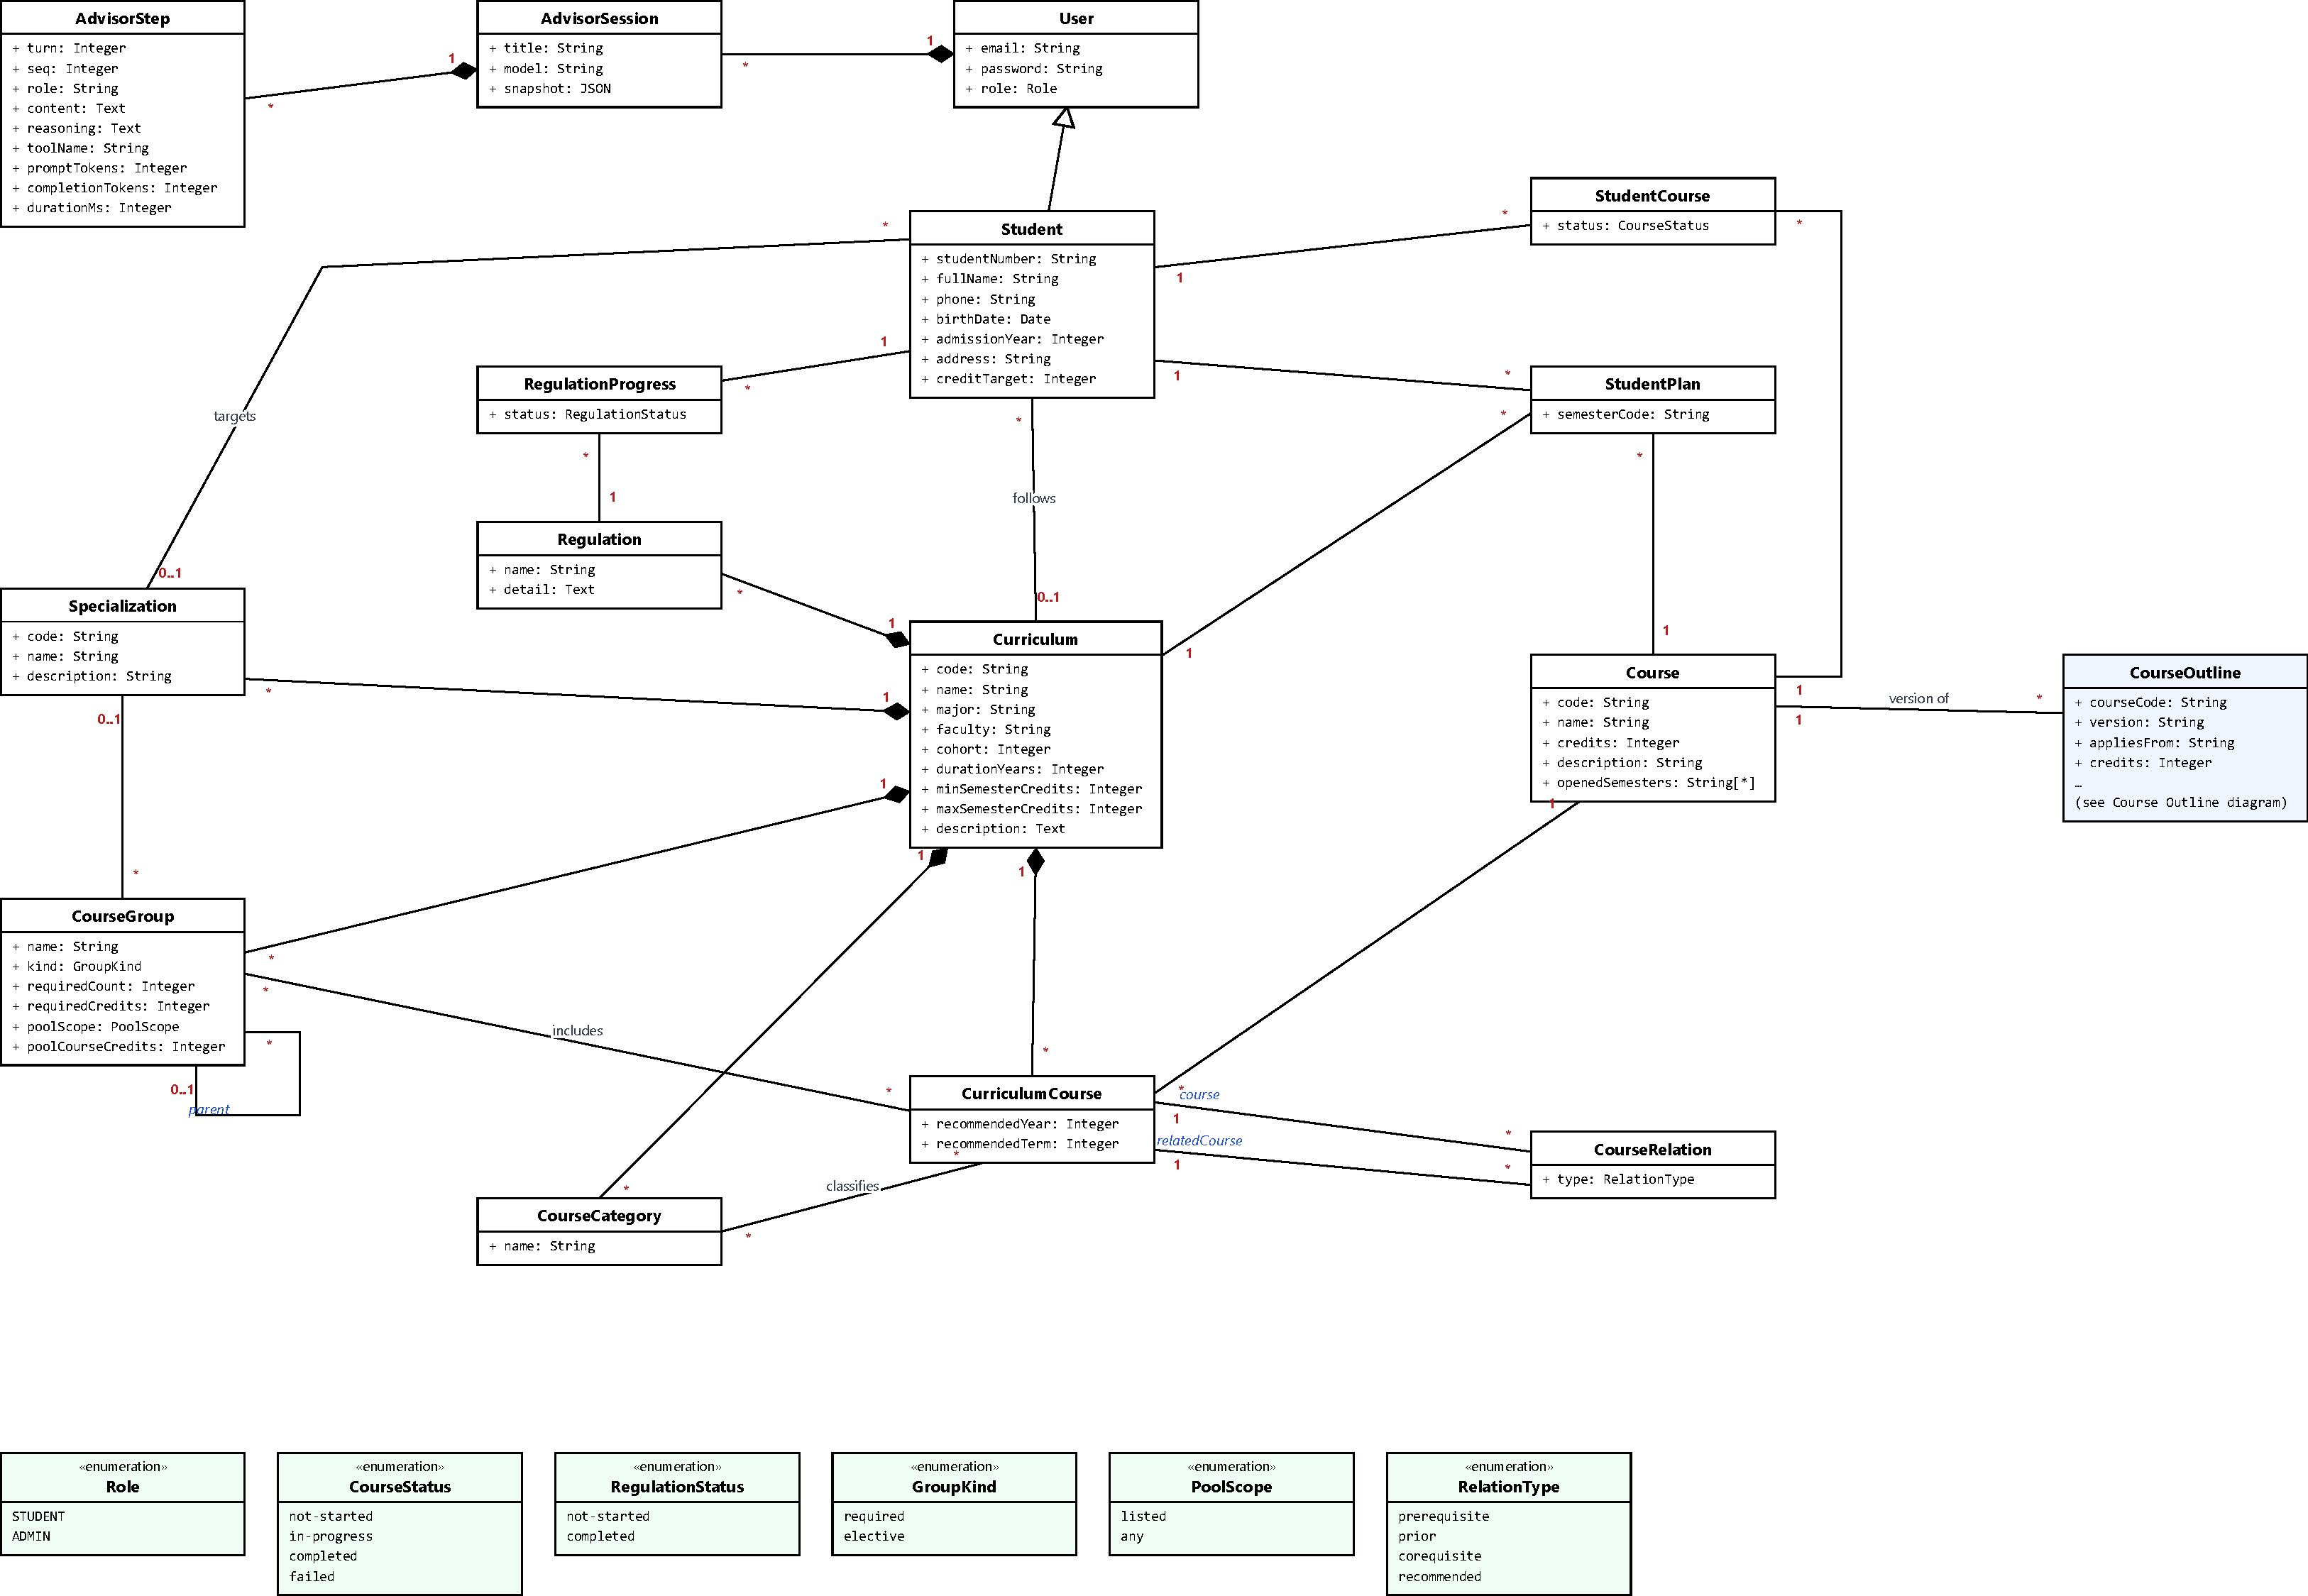
\includegraphics[width=\linewidth,height=0.9\textheight,keepaspectratio]{image/class-diagram.pdf}
        \caption{System overview class diagram}
        \label{fig:class-diagram}
    \end{figure}
\end{landscape}
\restoregeometry
\setlength{\headheight}{40pt} % restoregeometry resets the header height set in h_and_d.tex

% Class diagram on its own landscape page, without header and footer
\newgeometry{margin=1.2cm}
\begin{landscape}
    \thispagestyle{empty}
    \begin{figure}[p]
        \centering
        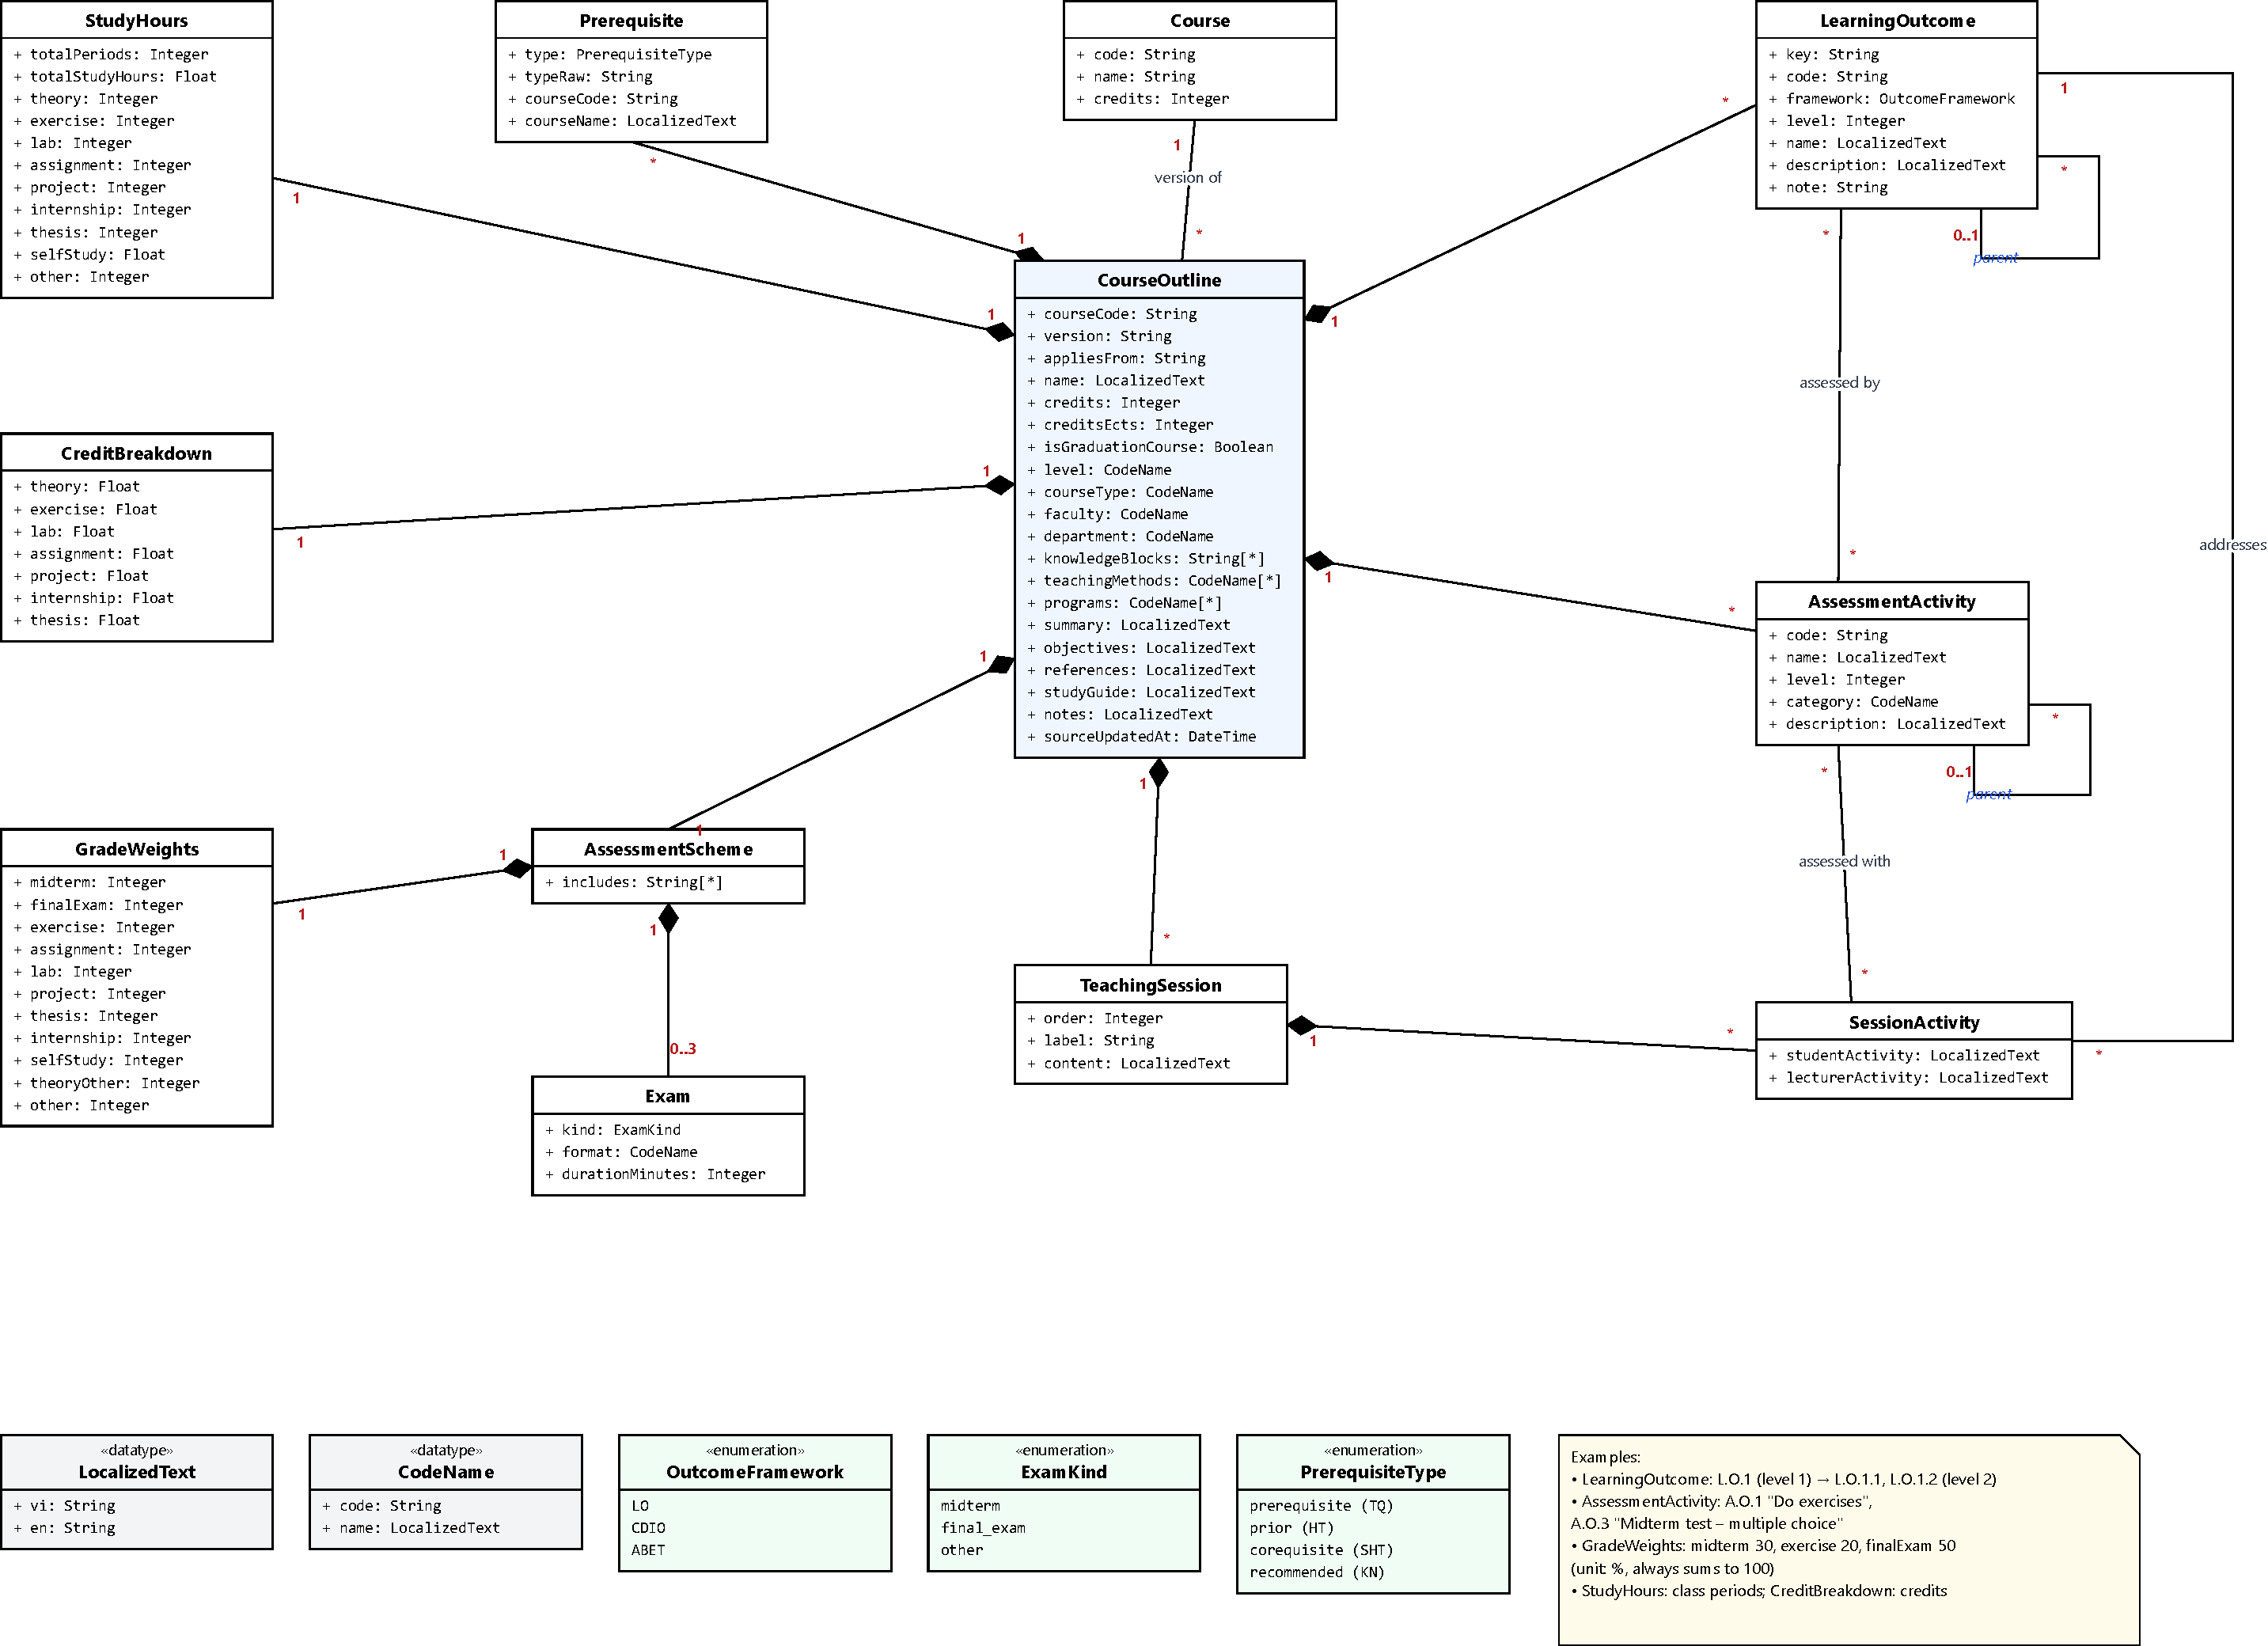
\includegraphics[width=\linewidth,height=0.9\textheight,keepaspectratio]{image/class-diagram-course-outline.pdf}
        \caption{Course outline class diagram}
        \label{fig:class-diagram-course-outline}
    \end{figure}
\end{landscape}
\restoregeometry
\setlength{\headheight}{40pt} % restoregeometry resets the header height set in h_and_d.tex

\section{System Design}
\label{sec:sys-design}

Building on the requirements and behavioural models identified in Section~\ref{sec:sys-analysis}, this section presents the proposed design of BK Uni and explains how each design decision addresses the needs of its stakeholders. It covers the system architecture, the database design and the user-interface design. Together, they form a clear specification for implementing a system that is correct with respect to curriculum rules, maintainable as curricula change, and able to explain its results to Students.

\subsection{Architecture Designs}
\label{subsec:architecture-design}

A platform such as BK Uni brings together several kinds of work that behave very differently: ordinary data management (profiles, curricula, course statuses), rule-based reasoning over a whole curriculum to analyze progress and recommend study plans, and conversational advising backed by a large language model. A well-defined architecture is needed to organize these concerns into one cohesive system. Without it, the dependencies between the curriculum data, the planning solvers that interpret academic rules, and the external AI service would quickly become difficult to reason about, test and evolve, which would directly threaten the correctness and explainability that the system promises.

This section presents the architecture of the platform: what software architecture means, the common architectural styles that were considered, the architectural decision made for BK Uni, and the resulting architecture design.

\subsubsection{Software Architectures}
\label{subsubsec:software-architecture}

Software architecture is the high-level structural design of a software system. It determines how the system is decomposed into components, how those components interact, how data flows between them, and how the system can grow over time. At its core, architecture is about the significant decisions that are difficult and costly to change later. For BK Uni, this means deciding, before any feature is implemented, where academic rules are evaluated, how curriculum and student data reach the planning solvers, and how the AI advisor is allowed to access that data.

Several authoritative definitions of software architecture are commonly cited:
\begin{itemize}
    \item \textbf{ISO/IEC/IEEE 42010:2011} (formerly IEEE 1471) defines architecture as the ``fundamental concepts or properties of a system in its environment embodied in its elements, relationships, and in the principles of its design and evolution''~\cite{iso42010}.
    \item \textbf{The Software Engineering Institute (SEI) at Carnegie Mellon University} describes it as the ``set of structures needed to reason about the system, which comprise software elements, relations among them, and properties of both''~\cite{bass-sei}.
    \item \textbf{The Open Group Architecture Framework (TOGAF)} gives two interpretations: (1) ``a formal description of a system, or a detailed plan of the system at component level to guide its implementation'', and (2) ``the structure of components, their inter-relationships, and the principles and guidelines governing their design and evolution over time''~\cite{togaf}.
    \item \textbf{Ralph Johnson}, one of the ``Gang of Four'', offers a pragmatic industry view, describing architecture as ``the decisions that you wish you could get right early in a project''~\cite{fowler-architect}.
\end{itemize}

Based on these definitions, software architecture can be characterized by three essential pillars:
\begin{itemize}
    \item \textbf{Structure:} the logical and physical components of the system and how they are organized and partitioned to manage complexity.
    \item \textbf{Behaviour:} the interaction patterns between components, including the protocols and data exchanged between them.
    \item \textbf{Quality attributes:} beyond functionality, the architecture must address non-functional requirements such as security, performance, reliability, maintainability and scalability (Section~\ref{sec:sys-analysis}).
\end{itemize}

\subsubsection{Common Architectural Styles}
\label{subsubsec:architecture-styles}

Selecting an architectural style is a critical decision because it determines how the platform handles data, isolates complex logic and scales over time. Architectural styles are generally divided into \emph{monolithic} styles, in which all components are deployed as a single unit, and \emph{distributed} styles, in which components are deployed separately and communicate over a network~\cite{richards-ford}.

\textbf{Monolithic architecture styles}
\begin{itemize}
    \item \textbf{Layered architecture (n-tier):}
    \begin{itemize}
        \item \textit{Definition:} organizes the application into horizontal layers (for example presentation, business, persistence and database), each with a specific role and interacting only with the layer directly below it.
        \item \textit{Best for:} small to medium applications where development speed matters and the domain is not overly complex.
    \end{itemize}
    \item \textbf{Pipeline architecture (pipe-and-filter):}
    \begin{itemize}
        \item \textit{Definition:} decomposes a task into a sequence of self-contained processing steps (filters) connected by channels (pipes).
        \item \textit{Best for:} systems dominated by data transformation, such as document processing, ETL jobs or compilers.
    \end{itemize}
    \item \textbf{Microkernel architecture (plug-in):}
    \begin{itemize}
        \item \textit{Definition:} consists of a minimal core system and a set of plug-in modules that provide specialized features or additional logic.
        \item \textit{Best for:} products in which custom extensions must be added without modifying the core.
    \end{itemize}
\end{itemize}

\textbf{Distributed architecture styles}
\begin{itemize}
    \item \textbf{Service-based architecture:}
    \begin{itemize}
        \item \textit{Definition:} a hybrid approach in which the application is split into a small number of coarse-grained, independently deployed services that typically share a single database.
        \item \textit{Best for:} systems that need to isolate a few distinct domains or runtimes without taking on the full operational complexity of a fine-grained distributed system.
    \end{itemize}
    \item \textbf{Event-driven architecture:}
    \begin{itemize}
        \item \textit{Definition:} an asynchronous style in which components communicate by producing and consuming events through a broker, yielding highly decoupled and reactive systems.
        \item \textit{Best for:} high-throughput systems with real-time updates or long-running asynchronous workflows.
    \end{itemize}
    \item \textbf{Microservices architecture:}
    \begin{itemize}
        \item \textit{Definition:} many small, fine-grained services, each owning its own database and communicating through lightweight protocols such as HTTP or gRPC.
        \item \textit{Best for:} large, complex systems that require independent scaling and deployment of many features and high fault tolerance.
    \end{itemize}
\end{itemize}

\subsubsection{Strategic Decision}
\label{subsubsec:architecture-decision}

Among the styles listed above, BK Uni adopts a \textbf{modular, layered monolith} for its server, extended with \textbf{out-of-process Python workers} for the CPU-bound work. The \emph{Backend Server} is a single deployable application that owns all business data and exposes every function of the system. When a request needs combinatorial search or document parsing, the Backend starts a short-lived Python process, the \emph{planner}, passes it the input as JSON on its standard input, and reads the result from its standard output. This keeps the operational simplicity of a monolith while isolating the parts that differ most from ordinary request handling, and it follows directly from the nature of the problem:
\begin{itemize}
    \item \textbf{Different runtimes and workloads.} The Backend Server performs short, I/O-bound operations (database reads and writes, calls to the AI service), for which Node.js is well suited. Building a study roadmap is a CPU-bound search over a whole curriculum, and the mature solvers for it, Google OR-Tools CP-SAT and \texttt{clingo}, are available in Python. Running each solving step in its own process keeps it from blocking the request-handling event loop, lets each part use the most suitable language, and allows the Backend to stop a solver that runs too long.
    \item \textbf{Separation of rules from application code.} The planning problem is defined once as a constraint satisfaction problem (Section~\ref{sec:formulation}) and implemented in the planner, not in the Backend. The planner has two interchangeable solver back-ends: a CP-SAT model, used by the Student interface, and an Answer Set Programming encoding (Section~\ref{sec:encoding}) solved by \texttt{clingo}, available through the same API for comparison. Rules can therefore be developed and tested in Python on fixed inputs without touching the rest of the application, which supports NFR-4.1 and NFR-4.2.
    \item \textbf{Stateless workers with a single data owner.} A planner process never accesses the database. It receives everything it needs for one request and exits after replying, so the Backend Server remains the only component that reads and writes persistent data and enforces authentication and data ownership on every request (NFR-1.1). This avoids the data-consistency and infrastructure overhead of a database per service, which matters for a small development team.
\end{itemize}

Within the Backend Server, the code follows a modular, layered design: each functional area (authentication, users, student data, curricula, courses, course outlines, planning and the AI advisor) is a self-contained module with its own controllers, services and data entities. This keeps responsibilities clear while avoiding the cost of splitting every module into its own service. Two kinds of work are deliberately kept out of the server. The \emph{progress analysis} of a Student is computed in the browser from data the Backend serves, because it must react instantly to unsaved edits on the course board. \emph{Data ingestion} follows the pipeline style: curricula and course outlines are fetched from the university's systems and transformed offline before being imported into the system.

An event-driven design with a message broker was deliberately not adopted at this stage. Planning requests are bounded in size, since a single curriculum contains a few hundred courses: the CP-SAT search is limited to 20 seconds and any planner process is stopped after 60 seconds. A synchronous request--response interaction is therefore simpler, easier to debug and sufficient. Because the Backend talks to the planner through a narrow JSON interface, the workers could later be moved behind a queue or onto separate machines without changing the Backend's business modules, should the load require it.

\subsubsection{Architecture Design}
\label{subsubsec:architecture-overview}

The design follows a client--server model in which a single-page frontend communicates with the Backend Server, and the Backend Server in turn delegates roadmap planning and report parsing to Python workers and conversational advising to an external language model. The design pursues three main goals: keeping the academic rules of planning in one place that can be tested independently; ensuring that persistent data is accessed and protected by exactly one component; and integrating the external AI service in a controlled way so that it can only use data the system provides.

Figure~\ref{fig:system-architecture} shows the overall architecture of BK Uni.

\begin{figure}[H]
    \centering
    % Fixed font sizes so the diagram does not depend on the 14pt body font
    \renewcommand{\small}{\fontsize{9}{11}\selectfont}%
    \renewcommand{\scriptsize}{\fontsize{7}{8.5}\selectfont}%
    \resizebox{\textwidth}{!}{%
    \begin{tikzpicture}[
        font=\small,
        >=stealth,
        comp/.style={draw, thick, align=center, fill=white, inner sep=3pt},
        ext/.style={comp, fill=gray!8},
        store/.style={draw, thick, cylinder, shape border rotate=90, aspect=0.22,
                      align=center, minimum width=3.2cm, minimum height=1.9cm, fill=white},
        flow/.style={->, thick},
        lbl/.style={font=\scriptsize, fill=white, inner sep=1.5pt, align=center},
      ]
      % ---------------- Containers ----------------
      \draw[thick] (2.6,10.1) rectangle (12.6,11.9);
      \draw[thick] (3.1,10.1) -- (3.1,11.9);
      \node[rotate=90, font=\bfseries\small] at (2.85,11.0) {Clients};
      \draw[thick] (2.6,5.4) rectangle (12.6,8.1);
      \draw[thick] (3.1,5.4) -- (3.1,8.1);
      \node[rotate=90, font=\bfseries\small] at (2.85,6.75) {Servers};
      \draw[thick] (13.4,7.9) rectangle (18.6,11.1);
      \draw[thick] (13.4,10.5) -- (18.6,10.5);
      \node[font=\bfseries\small] at (16.0,10.8) {External Services};

      % ---------------- Components ----------------
      \node[comp, minimum width=9.2cm, minimum height=1.3cm] (fe) at (7.85,11.0)
           {Frontend\\[-1pt]{\scriptsize (React single-page application for Students and Admins;}\\[-2pt]
            {\scriptsize progress analysis computed in the browser)}};

      \node[comp, minimum width=3.9cm, minimum height=2.2cm] (be) at (5.2,6.75)
           {Backend Server\\[-1pt]{\scriptsize (NestJS)}\\[1pt]
            {\scriptsize Auth $\cdot$ User $\cdot$ Student $\cdot$ Curriculum}\\[-2pt]
            {\scriptsize Course $\cdot$ Outline $\cdot$ Planner $\cdot$ Advisor}};

      \node[comp, minimum width=3.7cm, minimum height=2.2cm] (re) at (10.6,6.75)
           {Python Workers\\[-1pt]{\scriptsize (one process per request)}\\[1pt]
            {\scriptsize planner.cli: CP-SAT or clingo}\\[-2pt]
            {\scriptsize planner.mybk: progress reports}};

      \node[comp, minimum width=4.4cm, minimum height=1.8cm] (ds) at (16.0,9.3)
           {DeepSeek API\\[-1pt]{\scriptsize (large language model behind}\\[-2pt]{\scriptsize the AI academic advisor)}};

      \node[ext, minimum width=4.2cm, minimum height=1.8cm] (src) at (-0.5,11.0)
           {myBK\\[-1pt]{\scriptsize (university system: curriculum}\\[-2pt]{\scriptsize API, course outlines)}};

      \node[comp, minimum width=4.2cm, minimum height=2.7cm] (pl) at (-0.5,6.75)
           {Data Ingestion Scripts\\[-1pt]{\scriptsize (offline, Node.js)}\\[1pt]
            {\scriptsize fetch $\cdot$ normalize}\\[-2pt]
            {\scriptsize build import JSON}};

      \node[store] (db) at (4.8,2.3) {PostgreSQL\\Database};
      \node[store, minimum width=3.0cm] (es) at (7.9,2.3) {Search Index\\{\scriptsize (Elasticsearch,}\\[-2pt]{\scriptsize optional)}};
      \node[store] (asp) at (11.4,2.3) {Planning Rules\\{\scriptsize (CP-SAT model,}\\[-2pt]{\scriptsize ASP \texttt{.lp} files)}};

      % ---------------- Flows ----------------
      \draw[flow] (4.6,10.35) -- (4.6,7.85) node[lbl, pos=0.45] {RESTful APIs\\(HTTPS, session cookie)};
      \draw[flow] (7.15,7.15) -- (8.75,7.15) node[lbl, midway, above=1pt, fill=none] {JSON (stdin)};
      \draw[flow] (8.75,6.35) -- (7.15,6.35) node[lbl, midway, below=1pt, fill=none] {JSON (stdout)};
      \draw[flow] (6.4,7.85) |- (ds.west) node[lbl, pos=0.75] {RESTful APIs (tool calling)};
      \draw[flow] (4.8,5.65) -- (db.north) node[lbl, midway] {SQL queries\\(TypeORM)};
      \draw[flow] (7.0,5.65) -- (7.0,3.25) node[lbl, midway] {Outline\\search};
      \draw[flow] (asp.north) -- (11.4,5.65) node[lbl, midway] {Loaded by\\the solvers};
      \draw[flow] (src.south) -- (pl.north) node[lbl, midway] {Fetches JSON\\and outlines};
      \draw[flow] (pl.south) |- (3.5,4.4) -- (3.5,5.65);
      \node[lbl] at (1.5,4.4) {Admin import (RESTful APIs)};
    \end{tikzpicture}%
    }
    \caption{System architecture}
    \label{fig:system-architecture}
\end{figure}

\begin{itemize}
    \item \textbf{Clients (Frontend):} A single-page application built with React that serves as the only user interface for both Students and Admins. It communicates exclusively with the Backend Server through RESTful APIs over HTTPS; it never contacts the database, the Python workers or the AI service directly. Authentication relies on a session token stored in an HTTP-only cookie, so the token is never exposed to client-side scripts (NFR-1.3). Besides rendering, the frontend computes the Student's progress analysis (credit progress, course eligibility, outstanding requirements and personal-plan warnings) from the data the Backend serves, and keeps edits on the course board as a draft until the Student saves them. The interface adapts to the user's role, showing the course board, analysis, roadmap recommendations and the AI advisor to Students, and curriculum management screens to Admins.

    \item \textbf{Servers:} The processing layer consists of the Backend Server and the Python workers it starts:
    \begin{itemize}
        \item \textbf{Backend Server:} The central orchestrator, implemented with NestJS. It handles every client request, authenticates the user, checks role and data ownership, and validates input before any business logic runs; a rate limiter is configured for sign-in and AI requests and must be enabled in production. It is organized into modules: \emph{Auth} (registration, sign-in and server-side sessions), \emph{User}, \emph{Student} (profiles, course statuses, personal plans and regulation statuses), \emph{Curriculum} and \emph{Course} (curricula, elective groups, specializations, categories, course relations and offering history), \emph{Outline} (import and lookup of course outlines), \emph{Planner} (myBK progress import, saved planning scenarios and roadmap solving) and \emph{Advisor} (AI conversations). For a roadmap request, the Planner module loads the Student's record and the curriculum data, builds the solver input, and runs the planner process; for a myBK report, it passes the uploaded bytes to the report reader and stores the parsed progress in a transaction.
        \item \textbf{Python Workers:} Short-lived processes of the \texttt{planner} package, started by the Backend for each request and fed through standard input and output. \texttt{planner.cli} implements the formulation in Section~\ref{sec:formulation}: it normalizes the input, solves it with the CP-SAT model (or with the \texttt{clingo} ASP encoding when that engine is selected), validates the resulting roadmap against the curriculum rules, compares it with the Student's baseline roadmap, and returns the roadmap together with the reason for each course, the assumptions and the warnings. If no roadmap satisfies the constraints, it reports which of the Student's settings block it and proposes fixes instead of relaxing any rule (FR-5.6). \texttt{planner.mybk} reads a myBK progress report, either a PDF or pasted text, into structured JSON. The workers hold no state and no database credentials, so they can be tested in isolation on fixed inputs; the Backend stops any worker that has not replied within 60 seconds.
    \end{itemize}

    \item \textbf{Data and Rule Tier:}
    \begin{itemize}
        \item \textbf{Database:} A PostgreSQL database, with all tables grouped under a dedicated schema, which serves as the system of record for user accounts and sessions, student profiles and academic records, imported myBK progress, curricula, course outlines and import batches, and AI advisor conversations (Section~\ref{subsec:database-design}). Only the Backend Server connects to it, multi-step changes are executed in transactions so that data is never left partially updated (NFR-3.2), and database triggers record changes to curriculum data in an audit log (NFR-7).
        \item \textbf{Search Index:} An optional Elasticsearch index of the course outlines, rebuilt when outlines are imported. The AI advisor uses it for full-text search over outline content (accent-insensitive, with abbreviations and typo tolerance) and to find courses with similar content. When no index is configured, the Backend falls back to searching PostgreSQL, so the system works without it.
        \item \textbf{Planning Rules:} The rule base used by the workers: the CP-SAT model in Python and the ASP encodings in \texttt{.lp} files, which express curriculum structure, course relations, credit limits and graduation conditions in a curriculum-independent way. Curriculum-specific information is supplied as input at request time, so supporting a new curriculum requires new data rather than new rules.
    \end{itemize}

    \item \textbf{Data Ingestion Scripts:} An offline set of Node.js scripts that turns the university's published data into the system's import format. They read curricula and teaching plans from the public curriculum API of myBK and course outlines from its outline pages, normalize them, and build JSON files. Curricula are then created through the Backend's Admin APIs, and course outlines through the outline import API, which records every import batch and reports discrepancies between sources, so the data used for planning remains traceable to its origin. Because the scripts run outside the request path, a slow or failed download never affects users of the running system.

    \item \textbf{External Services:}
    \begin{itemize}
        \item \textbf{DeepSeek API:} The large language model behind the AI academic advisor (FR-7), accessed over RESTful APIs. The Backend Server does not give the model direct access to the database. Instead, it exposes a small set of read-only tools, such as retrieving parts of the Student's progress analysis, course details, offering history, course outlines and specialization information, and executes each tool call itself under the current Student's permissions. The model's final answer is returned through a structured submission tool, which allows the Backend to validate it before displaying it. If the service fails or is unavailable, the Backend reports the error instead of presenting a fabricated answer (FR-7.6, NFR-3.4).
    \end{itemize}
\end{itemize}

By establishing this architecture, BK Uni gains a structural foundation in which ordinary data management, roadmap planning and AI-assisted advising are cleanly separated yet coordinated by a single Backend Server. Planning rules live in one tested package, persistent data has exactly one owner, and the external AI service can only see what the system chooses to share. For these components to work together, however, they depend on a well-organized data foundation that can represent curricula, course rules and each Student's academic record precisely. The following section presents the Database Design, detailing the entities, indexes and relationships that support the system's analysis and planning logic.

\subsection{Database Design}
\label{subsec:database-design}

This section describes the conceptual data model of the BK Uni system, as illustrated in the entity--relationship diagram at the end of this section. All persistent data is stored in a PostgreSQL database under a dedicated schema named \texttt{bk\_uni}, which contains the tables and enumerated types of the system. The model is organized around a set of entity types that capture the main concepts of the system: user accounts and student profiles, the progress that students import from myBK, conversations with the AI advisor, curricula together with their specializations, course groups and categories, and course outlines along with the batches through which they are imported. Columns shared by every table, namely \texttt{id}, \texttt{created\_at}, \texttt{updated\_at} and \texttt{updated\_by}, serve purely technical purposes and are therefore omitted from the conceptual model, as are the migration-history table, the audit log that database triggers fill with changes to curriculum data (it has no foreign keys and is not part of the domain), and the provenance metadata of curricula (source system, identifiers, version, synchronization time, English name and introduction texts). Foreign keys are represented as relationships between entities rather than as attributes. The following subsections detail the entities, indexes and relationships of the database.

\subsubsection{Entity}
\label{subsubsec:db-entity}

The entities of the system fall into two categories. Strong entities exist independently and are identified by a surrogate \texttt{Id} of type UUID, complemented, where one is available, by a natural key such as a course code or a curriculum code. Weak entities, in contrast, cannot be identified on their own: each of them depends on an owner entity, carries a partial key that is unique only within that owner, and is removed together with the owner when the latter is deleted. The \texttt{STUDENT} entity is modelled as a subclass of \texttt{USER}, distinguished by the condition \texttt{Role = 'STUDENT'}, since only students possess a personal profile, a record of study progress and a study plan. The complete set of entity types, together with their keys and main attributes, is summarized in the table below.

\begingroup\small
\begin{longtable}{|p{0.25\textwidth}|p{0.21\textwidth}|p{0.14\textwidth}|p{0.30\textwidth}|}
\caption{Entity types of the BK Uni database}\label{tab:db-entities}\\
\hline
\textbf{Entity} & \textbf{Type} & \textbf{Key} & \textbf{Main attributes} \\
\hline
\endfirsthead
\hline
\textbf{Entity} & \textbf{Type} & \textbf{Key} & \textbf{Main attributes} \\
\hline
\endhead
USER & Strong (superclass) & Id, Email & Password, Role \\
\hline
STUDENT & Subclass of USER & (inherited) & Student number, full name, phone, birth date, admission year, address, credit target \\
\hline
AUTH\_\allowbreak{}SESSION & Strong & Id & Expiry time of a sign-in session \\
\hline
STUDENT\_\allowbreak{}PROGRESS\_\allowbreak{}IMPORT & Strong & Id & Format (PDF or text), official program code, source update date, parsed report and the Student's adjustments (JSON) \\
\hline
ADVISOR\_\allowbreak{}SESSION & Strong & Id & Title, model, analysis snapshot and its hash \\
\hline
ADVISOR\_\allowbreak{}STEP & Weak (owner: ADVISOR\_\allowbreak{}SESSION) & Partial: Seq & Turn, role, content, reasoning, tool call (id, name, arguments), data, token usage (prompt, completion, cache hit), duration \\
\hline
CURRICULUM & Strong & Id, Code & Name, major, faculty, cohort, duration in years, semester credit limits (min, max), description, total credits for graduation, whether a specialization is required \\
\hline
CURRICULUM\_\allowbreak{}SPECIALIZATION & Weak (owner: CURRICULUM) & Partial: Code & Name, description \\
\hline
CURRICULUM\_\allowbreak{}REGULATION & Strong & Id & Name, detail of a non-course graduation requirement \\
\hline
COURSE\_\allowbreak{}GROUP & Weak (owner: CURRICULUM) & Partial: Name & Kind (required / elective), required count, required credits, pool scope, pool course credits, recommended (year, term) \\
\hline
COURSE\_\allowbreak{}CATEGORY & Weak (owner: CURRICULUM) & Partial: Name & --- \\
\hline
CURRICULUM\_\allowbreak{}COURSE & Weak (owners: CURRICULUM, COURSE) & --- & Recommended year and term of a course within a curriculum \\
\hline
COURSE & Strong & Id, Code & Name, credits, description, \{opened semesters\} \\
\hline
COURSE\_\allowbreak{}OUTLINE\_\allowbreak{}IMPORT & Strong & Id & Channel, format version, source, generation time, part / parts, counters (received, created, updated, unchanged, skipped), issues \\
\hline
COURSE\_\allowbreak{}OUTLINE & Strong & Id, (Course code, Version) & Applies-from semester, name (vi, en), credits, level, course type, faculty, source (id, code, updated at), content and its hash, \{prerequisites\} \\
\hline
\end{longtable}
\endgroup

Among these entities, \texttt{CURRICULUM\_COURSE} deserves particular attention. Although it could at first be regarded as a plain many-to-many relationship between curricula and courses, it is modelled as an entity in its own right for two reasons. First, it carries its own attributes, namely the recommended year and term in which the course should be taken. Second, it participates in further relationships, since course groups, course categories and course relations all refer to a course \emph{within a specific curriculum} rather than to the course in general. Finally, the full content of a course outline is stored as a structured JSON document, whose internal organization is described by the class diagram of the course outline presented in the System Analysis section.

\subsubsection{Index}
\label{subsubsec:db-index}

Indexes support both the integrity rules of the data model and the most frequent queries issued by the application. In addition to the B-tree primary-key index that is created on the \texttt{id} column of every table, a set of secondary indexes is declared to enforce uniqueness constraints and to accelerate common lookups, such as signing in by email, listing the conversations of a student, or finding the course outline that applies in a given semester. Several of the unique indexes are defined on \texttt{lower(...)} expressions, so that codes and names remain unique regardless of letter case. Furthermore, the composite unique indexes on \texttt{(id, curriculum\_id)} act as targets for foreign keys declared in child tables, allowing a child row to reference its parent together with the curriculum and thereby guaranteeing that linked items always belong to the same curriculum. The secondary indexes currently declared in the database are listed in the table below.

\begingroup\small
\begin{longtable}{|p{0.26\textwidth}|p{0.27\textwidth}|p{0.10\textwidth}|p{0.27\textwidth}|}
\caption{Secondary indexes of the BK Uni database}\label{tab:db-indexes}\\
\hline
\textbf{Table} & \textbf{Columns} & \textbf{Unique} & \textbf{Purpose} \\
\hline
\endfirsthead
\hline
\textbf{Table} & \textbf{Columns} & \textbf{Unique} & \textbf{Purpose} \\
\hline
\endhead
users & email & Yes & One account per email; sign-in lookup \\
\hline
auth\_\allowbreak{}sessions & user\_\allowbreak{}id & No & List and revoke a user's sessions \\
\hline
auth\_\allowbreak{}sessions & expires\_\allowbreak{}at & No & Find expired sessions \\
\hline
student\_\allowbreak{}progress\_\allowbreak{}imports & user\_\allowbreak{}id & Yes & One imported progress per account \\
\hline
audit\_\allowbreak{}log & table\_\allowbreak{}name, row\_\allowbreak{}id; occurred\_\allowbreak{}at (BRIN) & No & History of one row; changes in a time range \\
\hline
advisor\_\allowbreak{}sessions & user\_\allowbreak{}id, updated\_\allowbreak{}at & No & List a student's conversations, most recent first \\
\hline
advisor\_\allowbreak{}steps & session\_\allowbreak{}id, seq & Yes & Ordered steps within a conversation \\
\hline
courses & lower(code) & Yes & Case-insensitive unique course code \\
\hline
courses & lower(code), lower(name) (GIN, trigram) & No & Search courses by part of their code or name \\
\hline
course\_\allowbreak{}opened\_\allowbreak{}semesters & course\_\allowbreak{}id, semester\_\allowbreak{}code & Yes & A course is opened at most once per semester \\
\hline
curricula & lower(code) & Yes & Case-insensitive unique curriculum code \\
\hline
curriculum\_\allowbreak{}courses & curriculum\_\allowbreak{}id, course\_\allowbreak{}id & Yes & A course appears at most once in a curriculum \\
\hline
curriculum\_\allowbreak{}specializations & curriculum\_\allowbreak{}id, lower(code) & Yes & Unique specialization code within a curriculum \\
\hline
curriculum\_\allowbreak{}specializations & id, curriculum\_\allowbreak{}id & Yes & Target of same-curriculum foreign keys \\
\hline
course\_\allowbreak{}groups & curriculum\_\allowbreak{}id, lower(name) & Yes & Unique group name within a curriculum \\
\hline
course\_\allowbreak{}groups & id, curriculum\_\allowbreak{}id & Yes & Target of same-curriculum foreign keys \\
\hline
course\_\allowbreak{}group\_\allowbreak{}members & group\_\allowbreak{}id, course\_\allowbreak{}id & Yes & A course appears at most once in a group \\
\hline
course\_\allowbreak{}categories & curriculum\_\allowbreak{}id, lower(name) & Yes & Unique category name within a curriculum \\
\hline
course\_\allowbreak{}categories & id, curriculum\_\allowbreak{}id & Yes & Target of same-curriculum foreign keys \\
\hline
course\_\allowbreak{}category\_\allowbreak{}members & category\_\allowbreak{}id, course\_\allowbreak{}id & Yes & A course appears at most once in a category \\
\hline
course\_\allowbreak{}relations & curriculum\_\allowbreak{}id, course\_\allowbreak{}id, related\_\allowbreak{}course\_\allowbreak{}id, type & Yes & No duplicate relation of the same type between two courses \\
\hline
student\_\allowbreak{}profiles & user\_\allowbreak{}id & Yes & One profile per user \\
\hline
student\_\allowbreak{}profiles & student\_\allowbreak{}number & Yes & Unique student number (when provided) \\
\hline
student\_\allowbreak{}courses & user\_\allowbreak{}id, course\_\allowbreak{}id & Yes & One status per student and course \\
\hline
student\_\allowbreak{}plan\_\allowbreak{}courses & user\_\allowbreak{}id, curriculum\_\allowbreak{}id, course\_\allowbreak{}id & Yes & A course is planned at most once per student and curriculum \\
\hline
student\_\allowbreak{}regulation\_\allowbreak{}statuses & user\_\allowbreak{}id, regulation\_\allowbreak{}id & Yes & One status per student and regulation \\
\hline
course\_\allowbreak{}outlines & course\_\allowbreak{}code, version & Yes & One outline per course version \\
\hline
course\_\allowbreak{}outlines & course\_\allowbreak{}code, applies\_\allowbreak{}from & No & Find the outline that applies to a course in a given semester \\
\hline
course\_\allowbreak{}outline\_\allowbreak{}prerequisites & outline\_\allowbreak{}id & No & Load the prerequisites of an outline \\
\hline
\end{longtable}
\endgroup

\subsubsection{Relationship}
\label{subsubsec:db-relationship}

This subsection describes the connections between the entities defined above. Each relationship is characterized by its cardinality ratio, such as 1\,:\,N or M\,:\,N, and by the participation of each entity involved. Participation is \emph{total} when every instance of an entity must take part in the relationship, which corresponds to a NOT NULL foreign key in the schema, and \emph{partial} otherwise. Relationships that connect a weak entity to its owner are referred to as identifying relationships. Besides the usual binary relationships, the model contains a ternary relationship, \texttt{PLANS}, which records the semester in which a student intends to take a course of a given curriculum, as well as recursive relationships, such as the one between a course group and its subgroups and the one between related courses of the same curriculum. The full set of relationships, together with their cardinalities and participation constraints, is summarized in the table below.

\begingroup\small
\begin{longtable}{|p{0.24\textwidth}|p{0.28\textwidth}|p{0.11\textwidth}|p{0.27\textwidth}|}
\caption{Relationship types of the BK Uni database}\label{tab:db-relationships}\\
\hline
\textbf{Relationship} & \textbf{Participants} & \textbf{Ratio} & \textbf{Participation / attributes} \\
\hline
\endfirsthead
\hline
\textbf{Relationship} & \textbf{Participants} & \textbf{Ratio} & \textbf{Participation / attributes} \\
\hline
\endhead
HAS\_\allowbreak{}SESSION & USER -- AUTH\_\allowbreak{}SESSION & 1\,:\,N & Session total \\
\hline
UPLOADS & USER -- STUDENT\_\allowbreak{}PROGRESS\_\allowbreak{}IMPORT & 1\,:\,1 & Import total \\
\hline
STARTS & USER -- ADVISOR\_\allowbreak{}SESSION & 1\,:\,N & Advisor session total \\
\hline
HAS\_\allowbreak{}STEP (identifying) & ADVISOR\_\allowbreak{}SESSION -- ADVISOR\_\allowbreak{}STEP & 1\,:\,N & Step total \\
\hline
CREATES & USER -- COURSE\_\allowbreak{}OUTLINE\_\allowbreak{}IMPORT & 1\,:\,N & Both partial \\
\hline
PRODUCES & COURSE\_\allowbreak{}OUTLINE\_\allowbreak{}IMPORT -- COURSE\_\allowbreak{}OUTLINE & 1\,:\,N & Both partial \\
\hline
FOLLOWS & STUDENT -- CURRICULUM & N\,:\,1 & Both partial \\
\hline
TARGETS & STUDENT -- CURRICULUM\_\allowbreak{}SPECIALIZATION & N\,:\,1 & Both partial \\
\hline
COMPLETES & STUDENT -- CURRICULUM\_\allowbreak{}REGULATION & M\,:\,N & Both partial; attribute Status \\
\hline
TAKES & STUDENT -- COURSE & M\,:\,N & Both partial; attribute Status \\
\hline
PLANS (ternary) & STUDENT -- CURRICULUM -- COURSE & M\,:\,N\,:\,P & All partial; attribute Semester code \\
\hline
DEFINES & CURRICULUM -- CURRICULUM\_\allowbreak{}REGULATION & 1\,:\,N & Regulation total \\
\hline
HAS\_\allowbreak{}SPECIALIZATION (identifying) & CURRICULUM -- CURRICULUM\_\allowbreak{}SPECIALIZATION & 1\,:\,N & Specialization total \\
\hline
HAS\_\allowbreak{}GROUP (identifying) & CURRICULUM -- COURSE\_\allowbreak{}GROUP & 1\,:\,N & Group total \\
\hline
HAS\_\allowbreak{}CATEGORY (identifying) & CURRICULUM -- COURSE\_\allowbreak{}CATEGORY & 1\,:\,N & Category total \\
\hline
IN\_\allowbreak{}CURRICULUM (identifying) & CURRICULUM -- CURRICULUM\_\allowbreak{}COURSE & 1\,:\,N & Curriculum course total \\
\hline
OF\_\allowbreak{}COURSE (identifying) & COURSE -- CURRICULUM\_\allowbreak{}COURSE & 1\,:\,N & Curriculum course total \\
\hline
BELONGS\_\allowbreak{}TO & COURSE\_\allowbreak{}GROUP -- CURRICULUM\_\allowbreak{}SPECIALIZATION & N\,:\,1 & Both partial \\
\hline
SUBGROUP\_\allowbreak{}OF (recursive) & COURSE\_\allowbreak{}GROUP (Parent / Subgroup) & 1\,:\,N & Both partial \\
\hline
INCLUDES & COURSE\_\allowbreak{}GROUP -- CURRICULUM\_\allowbreak{}COURSE & M\,:\,N & Both partial \\
\hline
CLASSIFIES & COURSE\_\allowbreak{}CATEGORY -- CURRICULUM\_\allowbreak{}COURSE & M\,:\,N & Both partial \\
\hline
RELATES\_\allowbreak{}TO (recursive) & CURRICULUM\_\allowbreak{}COURSE (Course / Related course) & M\,:\,N & Both partial; multivalued attribute \{Type\}: prerequisite, prior, corequisite, recommended \\
\hline
\end{longtable}
\endgroup

In addition to the relationships above, several business rules cannot be expressed directly in the diagram. These rules are enforced either by constraints in the database or by checks in the application layer, as described below:
\begin{itemize}
    \item \textbf{Same curriculum.} A course group and its parent group, a group and its specialization, the members of a group or category, and both ends of a course relation must belong to the same curriculum. This is enforced by composite foreign keys on \texttt{(\ldots, curriculum\_id)}.
    \item \textbf{Subgroups.} A course group has a parent group if and only if it belongs to a specialization (check constraint \texttt{CHK\_course\_group\_specialization\_parent}).
    \item \textbf{Application checks.} A student's target specialization should belong to the curriculum the student follows, and a planned course should be part of that curriculum. These rules are checked by the application, not by the database.
    \item \textbf{Course outlines.} A course outline refers to its course by course code (stored in upper case). Its applies-from semester has the form \texttt{YY[1-3]}.
\end{itemize}

\subsubsection{ERD}
\label{subsubsec:db-erd}

The entities and relationships described above are brought together in the entity--relationship diagram shown on the following page. In this diagram, entity types are drawn as rectangles and relationship types as diamonds, with double borders marking weak entities and their identifying relationships. Attributes are drawn as ellipses: key attributes are underlined, partial keys carry a dashed underline, and multivalued attributes are enclosed by a double border. Double lines indicate total participation, while the numbers placed on each line give the cardinality ratio of the corresponding relationship. Finally, the \(\cup\)-shaped mark on the line between \texttt{USER} and \texttt{STUDENT} denotes the subclass relationship between these two entities.

% ERD on its own landscape page, without header and footer
\newgeometry{margin=1.2cm}
\begin{landscape}
    \thispagestyle{empty}
    \begin{figure}[p]
        \centering
        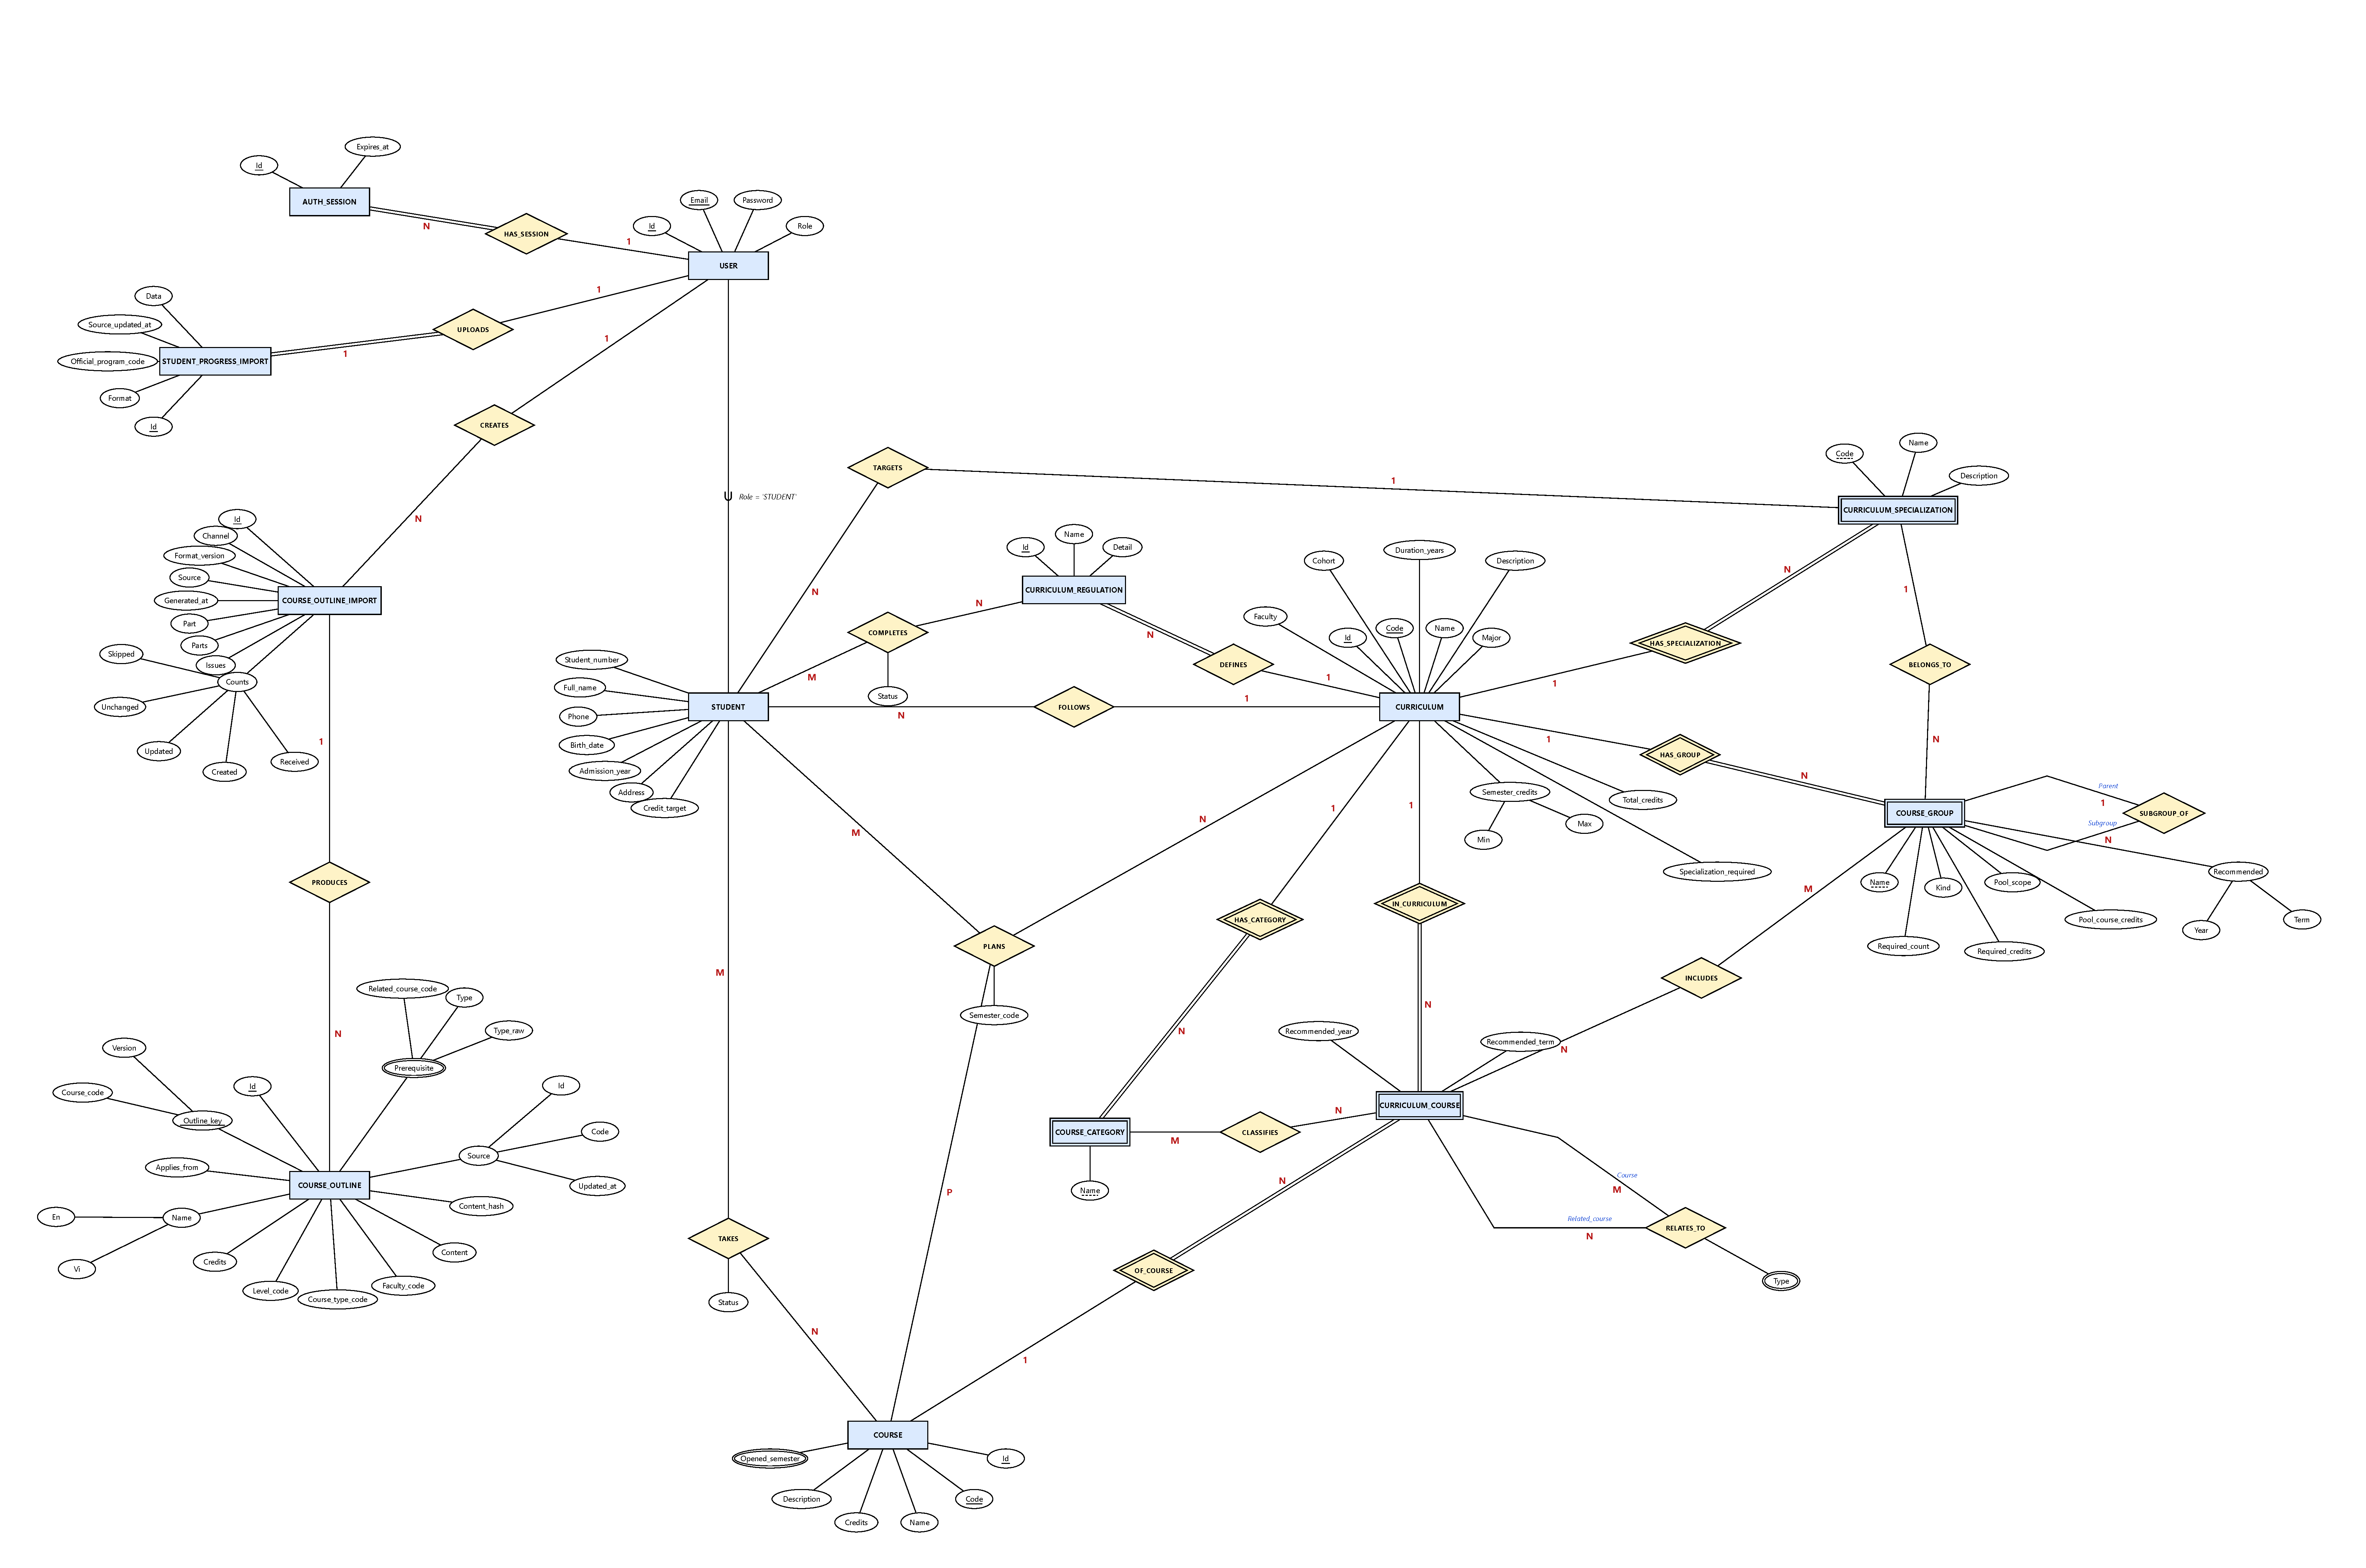
\includegraphics[width=\linewidth,height=0.9\textheight,keepaspectratio]{image/erd-chen.pdf}
        \caption{Entity--relationship diagram of the BK Uni database}
        \label{fig:erd}
    \end{figure}
\end{landscape}
\restoregeometry
\setlength{\headheight}{40pt} % restoregeometry resets the header height set in h_and_d.tex

\subsection{User Interface Designs}
\label{subsec:ui-design}

The final part of the System Design presents the user interface (UI) of BK Uni. As an academic planning assistant for students of Ho Chi Minh City University of Technology, the interface is designed with a strong focus on clarity and on keeping the data that students care about---their curriculum, their course statuses and their progress towards graduation---always one click away. Every student page shares the same layout: a sidebar on the left that groups the functions under \emph{Học tập} (Studying) and \emph{Tài khoản} (Account), a header bar showing the signed-in account, a light/dark theme switch and a sign-out button, and a content area where each page starts with a title, a short explanation of what the page is based on, and its main actions.

At the same time, the UI must stay faithful to the official sources used at the university. Course outlines imported from myBK are shown with the same structure as the original documents, including their version and source, and every figure computed by the system, such as remaining credits or the projected graduation semester, is accompanied by a note explaining how it was derived. In this way, students can trust the information and check it against the university's regulations before registering for courses. The screenshots in this section were captured from the running system using a demo account of a fourth-year Computer Science student (curriculum \texttt{CS-2023-KHMT}, admission year 2023, currently in semester 261).

\subsubsection{Flow Summary}
\label{subsubsec:ui-flow}

To summarize the normal user flow, we present the diagram in Figure~\ref{fig:ui-flow}, showing how a student navigates through BK Uni from signing in to finalizing a study plan. A new student first creates an account on the Register Page and then signs in on the Login Page, after which the system opens the Course List Page. If no curriculum has been selected yet, the pages remind the student to complete the Personal Profile first, since every analysis depends on the curriculum. The student then declares the status and planned semester of each course, opens the Course Detail Page whenever more information about a course is needed, and reviews the overall progress on the Learning Analysis Page. For questions that the analysis alone cannot answer, the student can consult the AI Advisor. Based on what they learn, students return to the Course List Page to adjust their plan, and this loop is repeated until the plan is finalized.

\begin{figure}[H]
    \centering
    \resizebox{!}{0.82\textheight}{%
    \begin{tikzpicture}[
        node distance=0.75cm and 1.1cm,
        font=\small,
        >=stealth,
        box/.style={rectangle, draw, text width=4.4cm, align=center, minimum height=1.1cm, execute at begin node={\hyphenpenalty=10000\relax}},
        term/.style={box, rounded corners=8pt},
        dec/.style={diamond, draw, aspect=2.4, text width=2.7cm, align=center, inner sep=1pt},
        arr/.style={->, thick},
        lbl/.style={font=\footnotesize, fill=white, inner sep=1.5pt}
    ]
        \node[term] (start) {Lands on the \textbf{Login Page}};
        \node[dec, below=of start] (acc) {Has an account?};
        \node[box, left=of acc] (reg) {Creates an account on the \textbf{Register Page}};
        \node[box, below=of acc] (signin) {Signs in with email and password};
        \node[box, below=of signin] (list) {Navigates to the \textbf{Course List Page}};
        \node[dec, below=of list] (cur) {Curriculum selected?};
        \node[box, left=of cur] (prof) {Fills in personal information and selects the curriculum on the \textbf{Personal Profile Page}};
        \node[box, below=of cur] (declare) {Declares course statuses and planned semesters on the \textbf{Course List Page}};
        \node[dec, below=of declare] (det) {Wants to view a course in detail?};
        \node[box, right=of det] (detail) {Views the outline and opening history on the \textbf{Course Detail Page}};
        \node[box, below=of det] (ana) {Reviews progress, missing courses and options on the \textbf{Learning Analysis Page}};
        \node[dec, below=of ana] (adv) {Needs further advice?};
        \node[box, below=of adv] (ai) {Chats with the AI on the \textbf{AI Advisor Page} and checks its \textbf{Trajectory}};
        \node[dec, below=of ai] (fin) {Study plan finalized?};
        \node[term, below=of fin] (end) {End};

        \draw[arr] (start) -- (acc);
        \draw[arr] (acc) -- node[lbl] {Yes} (signin);
        \draw[arr] (acc) -- node[lbl] {No} (reg);
        \draw[arr] (reg) |- (signin);
        \draw[arr] (signin) -- (list);
        \draw[arr] (list) -- (cur);
        \draw[arr] (cur) -- node[lbl] {Yes} (declare);
        \draw[arr] (cur) -- node[lbl] {No} (prof);
        \draw[arr] (prof) |- (list);
        \draw[arr] (declare) -- (det);
        \draw[arr] (det) -- node[lbl] {Yes} (detail);
        \draw[arr] (detail.north) |- ([yshift=-2mm]declare.east);
        \draw[arr] (det) -- node[lbl] {No} (ana);
        \draw[arr] (ana) -- (adv);
        \draw[arr] (adv) -- node[lbl] {Yes} (ai);
        \draw[arr] (adv.west) -- node[lbl, pos=0.5] {No} ++(-1.4,0) |- (fin.west);
        \draw[arr] (ai) -- (fin);
        \draw[arr] (fin) -- node[lbl] {Yes} (end);
        \draw[arr] (fin.east) -- node[lbl, pos=0.12] {No} ($(fin.east -| detail.east)+(0.8,0)$) |- ([yshift=2mm]declare.east);
    \end{tikzpicture}%
    }
    \caption{UI flow of a student in BK Uni}
    \label{fig:ui-flow}
\end{figure}

In the following subsections, the main pages of this flow are described in turn, together with the design decisions behind them.

\subsubsection{Course List Page}
\label{subsubsec:ui-course-list}

After signing in, students land on the \emph{Môn học \& kế hoạch} (Courses \& Plan) page, shown in Figure~\ref{fig:ui-courses}. To give an overview at a glance, the top of the page contains four summary cards: the number of courses the student has declared, the number of completed courses over the number of required ones, the accumulated credits over the credits required for graduation, and the credits already placed in the study plan. Below them, the \emph{Kế hoạch theo học kỳ} (Plan by semester) card groups the planned courses by the semester in which the student intends to take them.

\begin{figure}[H]
    \centering
    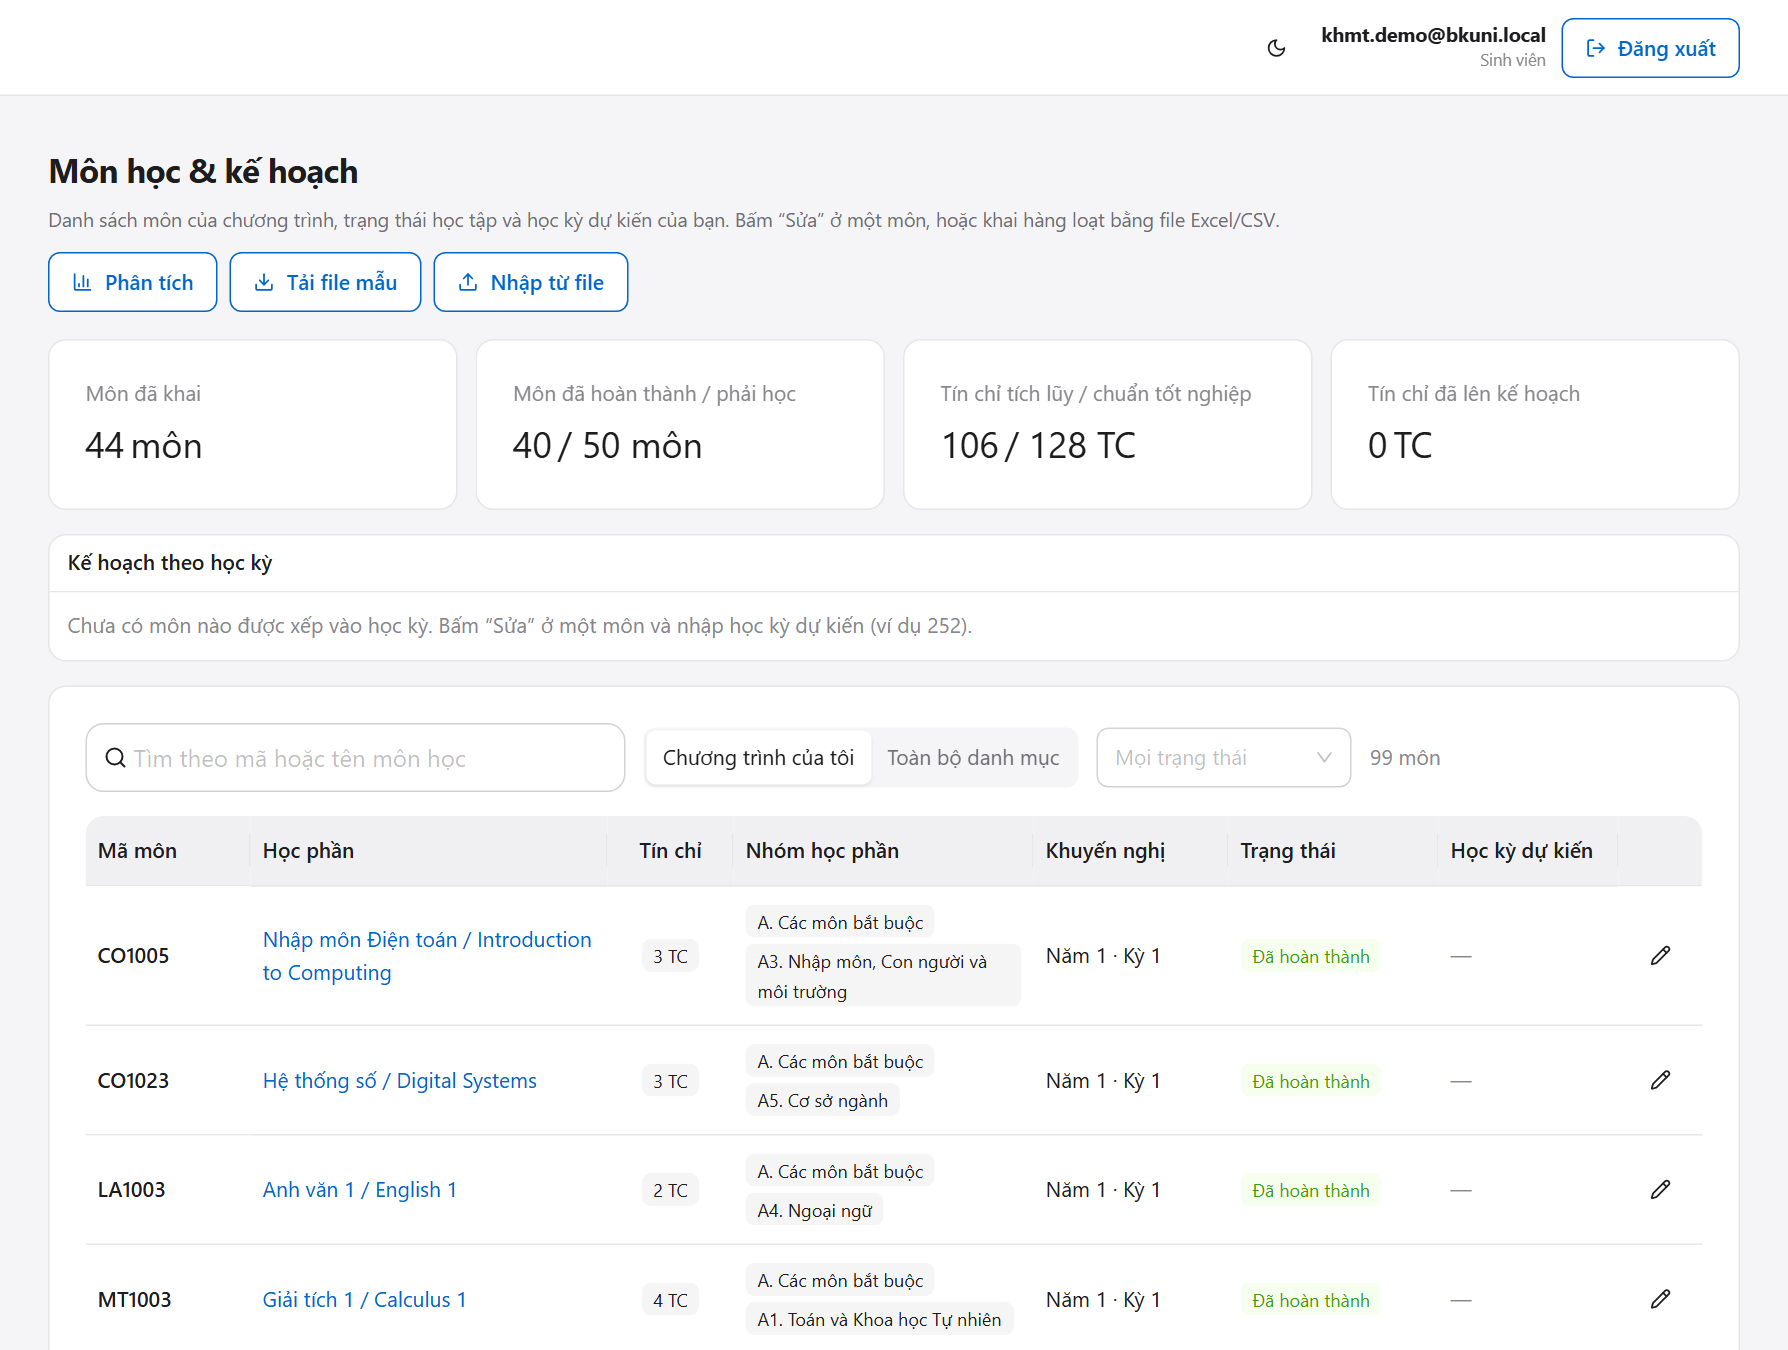
\includegraphics[width=\textwidth]{image/ui/courses.png}
    \caption{The Course List page}
    \label{fig:ui-courses}
\end{figure}

The main part of the page is the course table. Students can search by course code or name, switch between the courses of their own curriculum and the whole course catalog, and filter by learning status. Each row shows the course code and name, the number of credits, the course groups it belongs to, the recommended year and term according to the curriculum, the current status and the planned semester. Clicking the pencil icon at the end of a row lets the student update the status and planned semester of a single course, while the \emph{Tải file mẫu} (Download template) and \emph{Nhập từ file} (Import from file) buttons allow declaring many courses at once through an Excel/CSV file. The \emph{Phân tích} (Analysis) button leads to the Learning Analysis page described in Section~\ref{subsubsec:ui-analysis}.

\subsubsection{Course Detail Page}
\label{subsubsec:ui-course-detail}

Selecting a course name in the table navigates the student to the Course Detail page. The page is divided into two cards. The upper card summarizes the course within the student's curriculum: its code, name, credits, course groups, the student's own learning status and the time it was last updated. The lower card, \emph{Đề cương môn học} (Course outline), displays the outline imported from myBK. Its header contains a switch between Vietnamese and English and a selector of outline versions, in which the version that applies to the current semester is marked as \emph{Đang áp dụng} (In effect). Under the header, the general information of the outline---faculty, department, level, course type and knowledge block---is listed together with the source document and its update date. The content of the outline is then organized into six tabs so that students can jump directly to the part they need. Figure~\ref{fig:ui-detail-intro} shows the page with the first tab, \emph{Giới thiệu} (Introduction), opened for the course \texttt{CO1005}; this tab presents the course objectives, a short summary, study guidelines and the list of textbooks and references.

\begin{figure}[H]
    \centering
    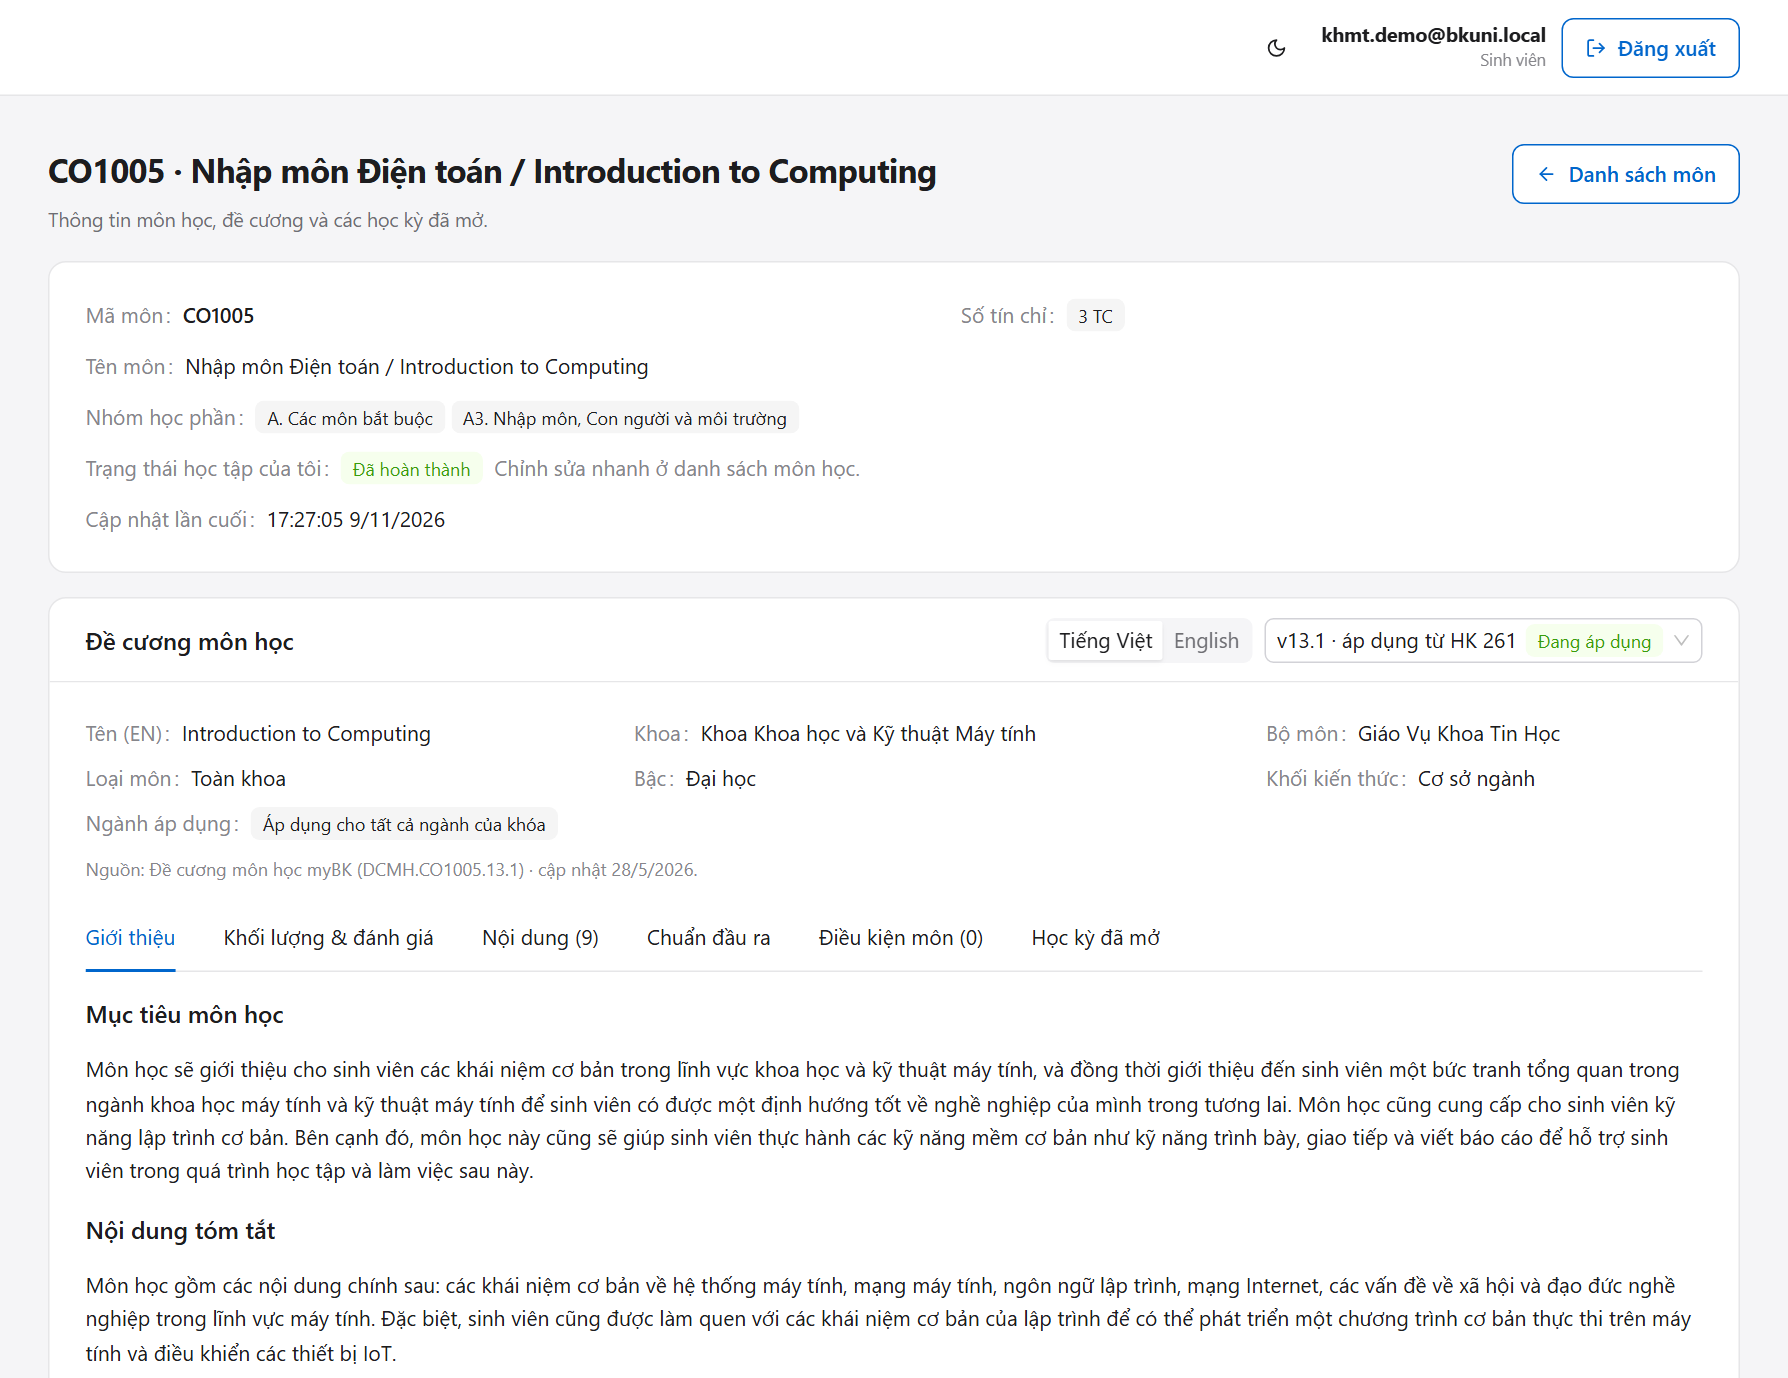
\includegraphics[width=\textwidth]{image/ui/detail-intro.png}
    \caption{The Course Detail page with the Introduction tab}
    \label{fig:ui-detail-intro}
\end{figure}

The \emph{Khối lượng \& đánh giá} (Workload \& Assessment) tab, shown in Figure~\ref{fig:ui-detail-workload}, turns the numbers in the outline into simple bar charts. On the left, the grading scheme shows the weight of each assessment component together with the format and duration of the midterm and final exams. On the right, the study workload shows the total number of periods, the estimated study hours and ECTS credits, and the breakdown into theory, laboratory, assignments, self-study and other activities. This helps students estimate how demanding a course is before choosing it.

\begin{figure}[H]
    \centering
    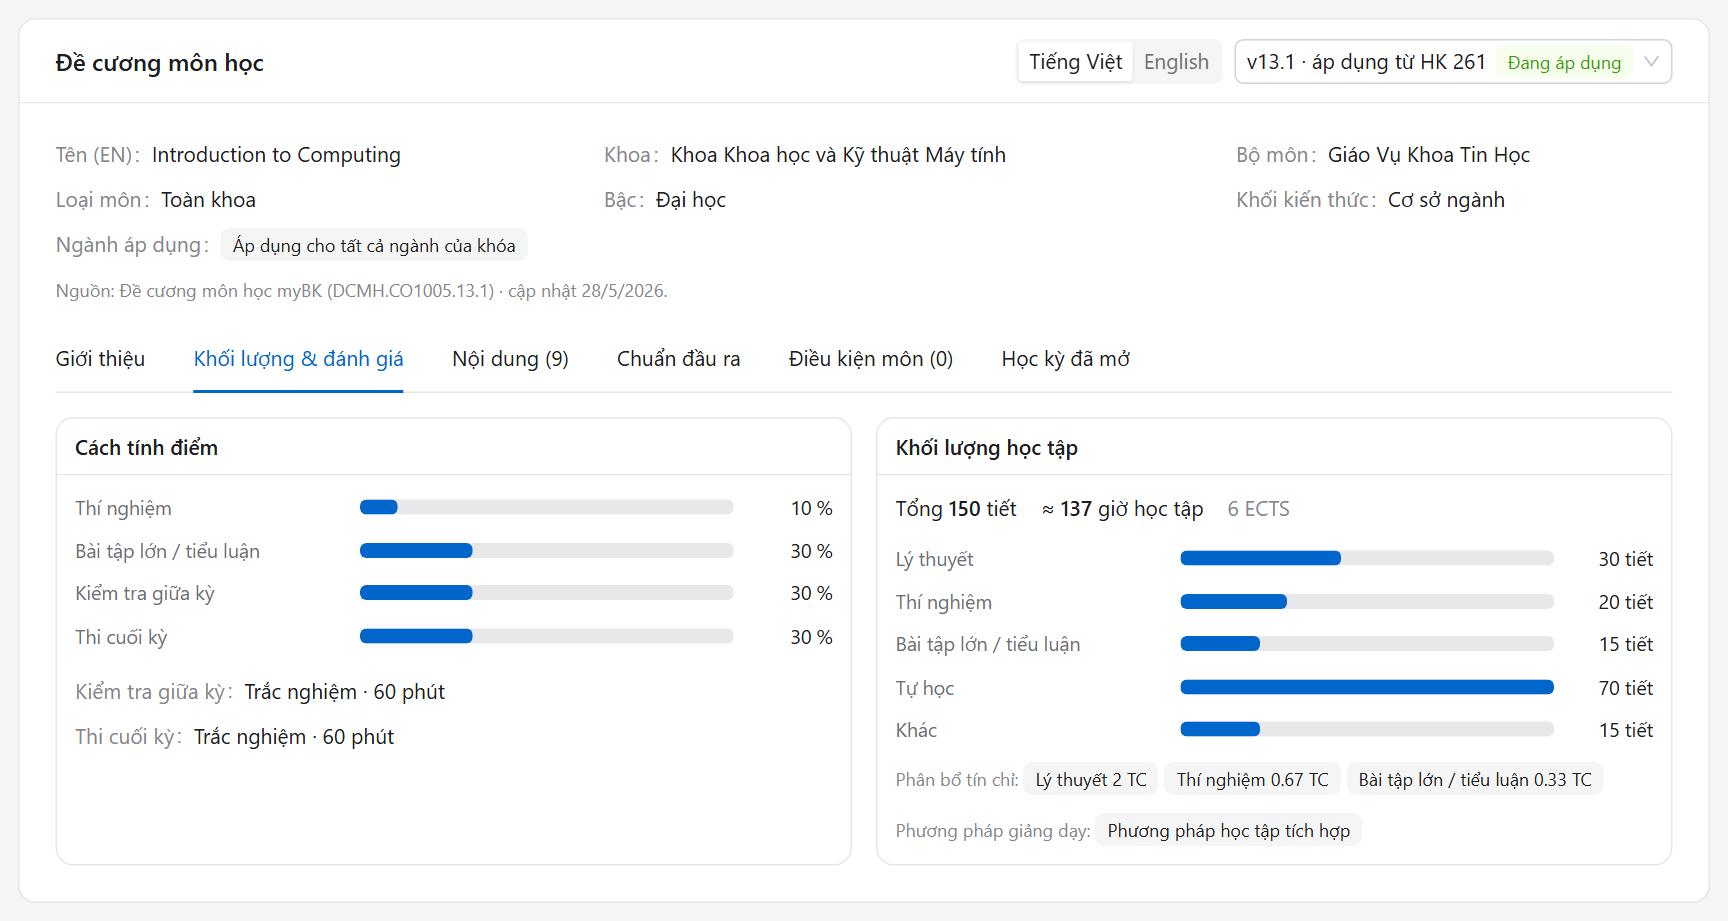
\includegraphics[width=0.9\textwidth]{image/ui/detail-workload.png}
    \caption{The Workload \& Assessment tab}
    \label{fig:ui-detail-workload}
\end{figure}

The \emph{Nội dung} (Content) tab, illustrated in Figure~\ref{fig:ui-detail-sessions}, lists the teaching sessions of the course in order; the number in the tab label indicates the number of session blocks. Each block shows the range of sessions it covers, the topics taught, the activities expected from students, and two kinds of tags: blue tags for the learning outcomes achieved in the block and yellow tags for the related assessment activities. Hovering over a tag reveals its full description.

\begin{figure}[H]
    \centering
    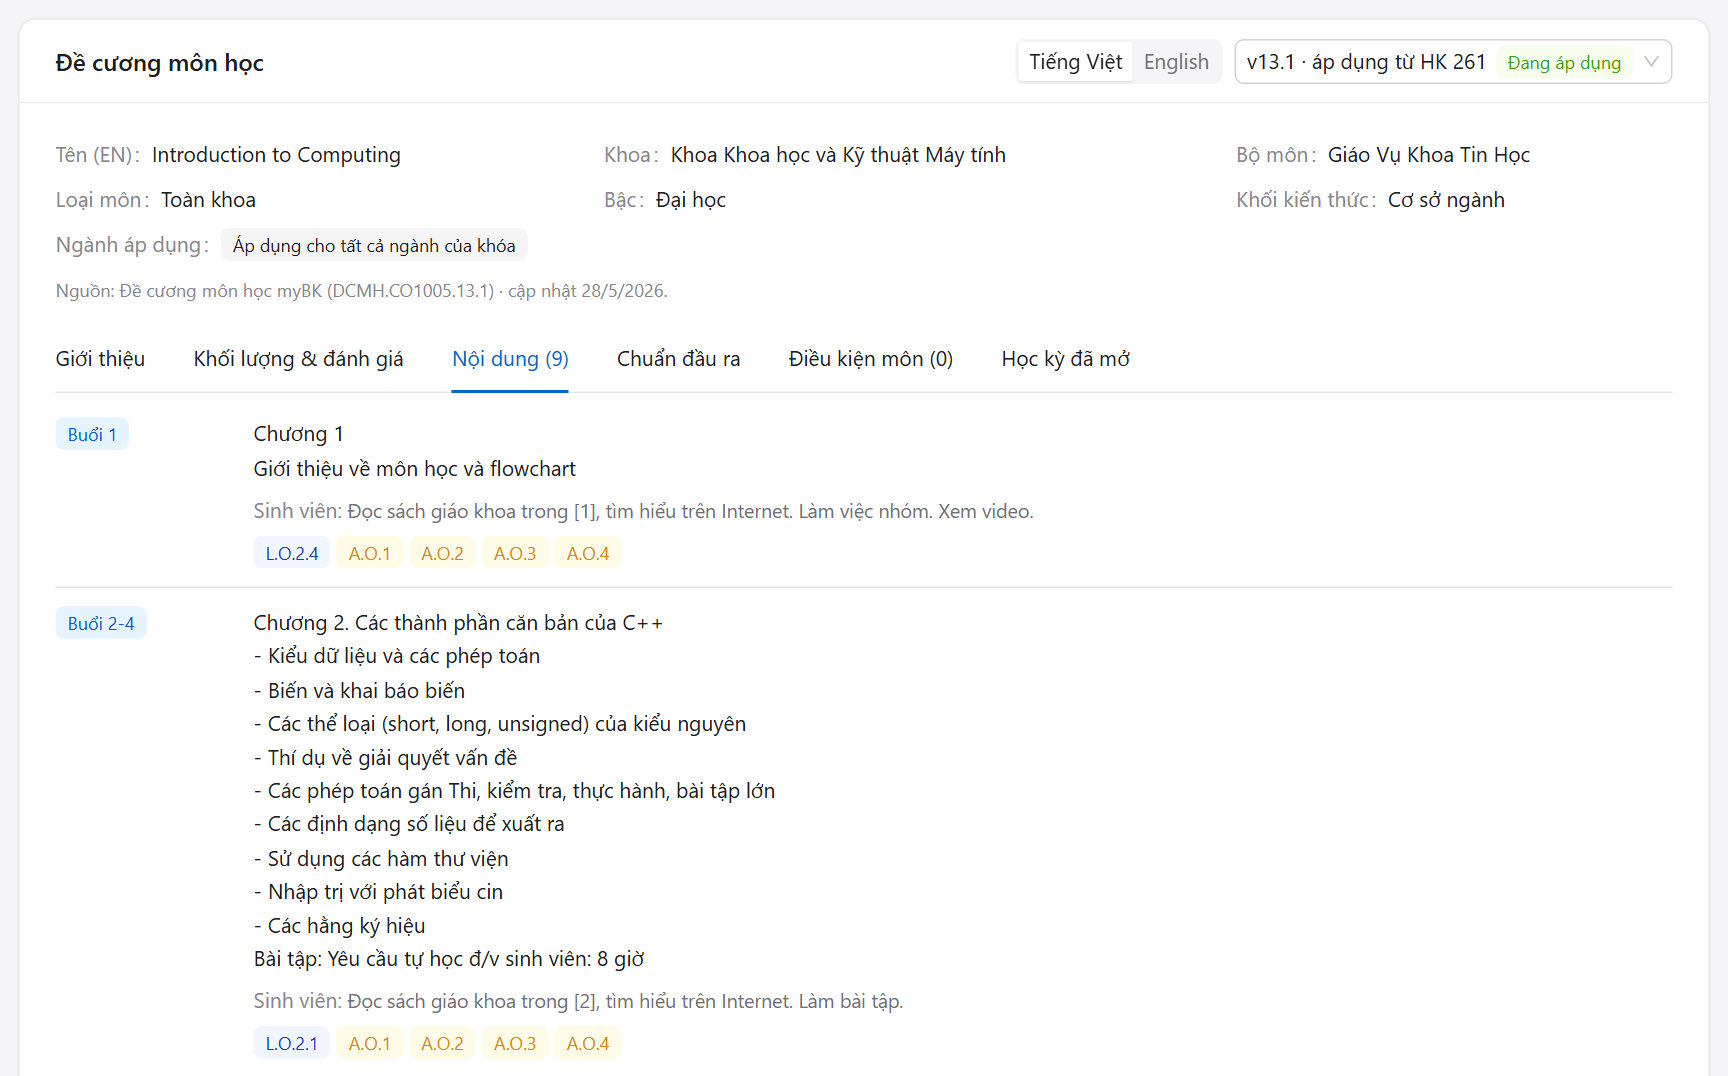
\includegraphics[width=0.9\textwidth]{image/ui/detail-sessions.png}
    \caption{The Content tab listing the teaching sessions}
    \label{fig:ui-detail-sessions}
\end{figure}

The \emph{Chuẩn đầu ra} (Learning Outcomes) tab, shown in Figure~\ref{fig:ui-detail-outcomes}, presents the learning outcomes of the course as a hierarchy, in which each detailed outcome is linked to the assessment activities used to evaluate it. The list of assessment activities and their corresponding forms of evaluation is given at the bottom of the tab.

\begin{figure}[H]
    \centering
    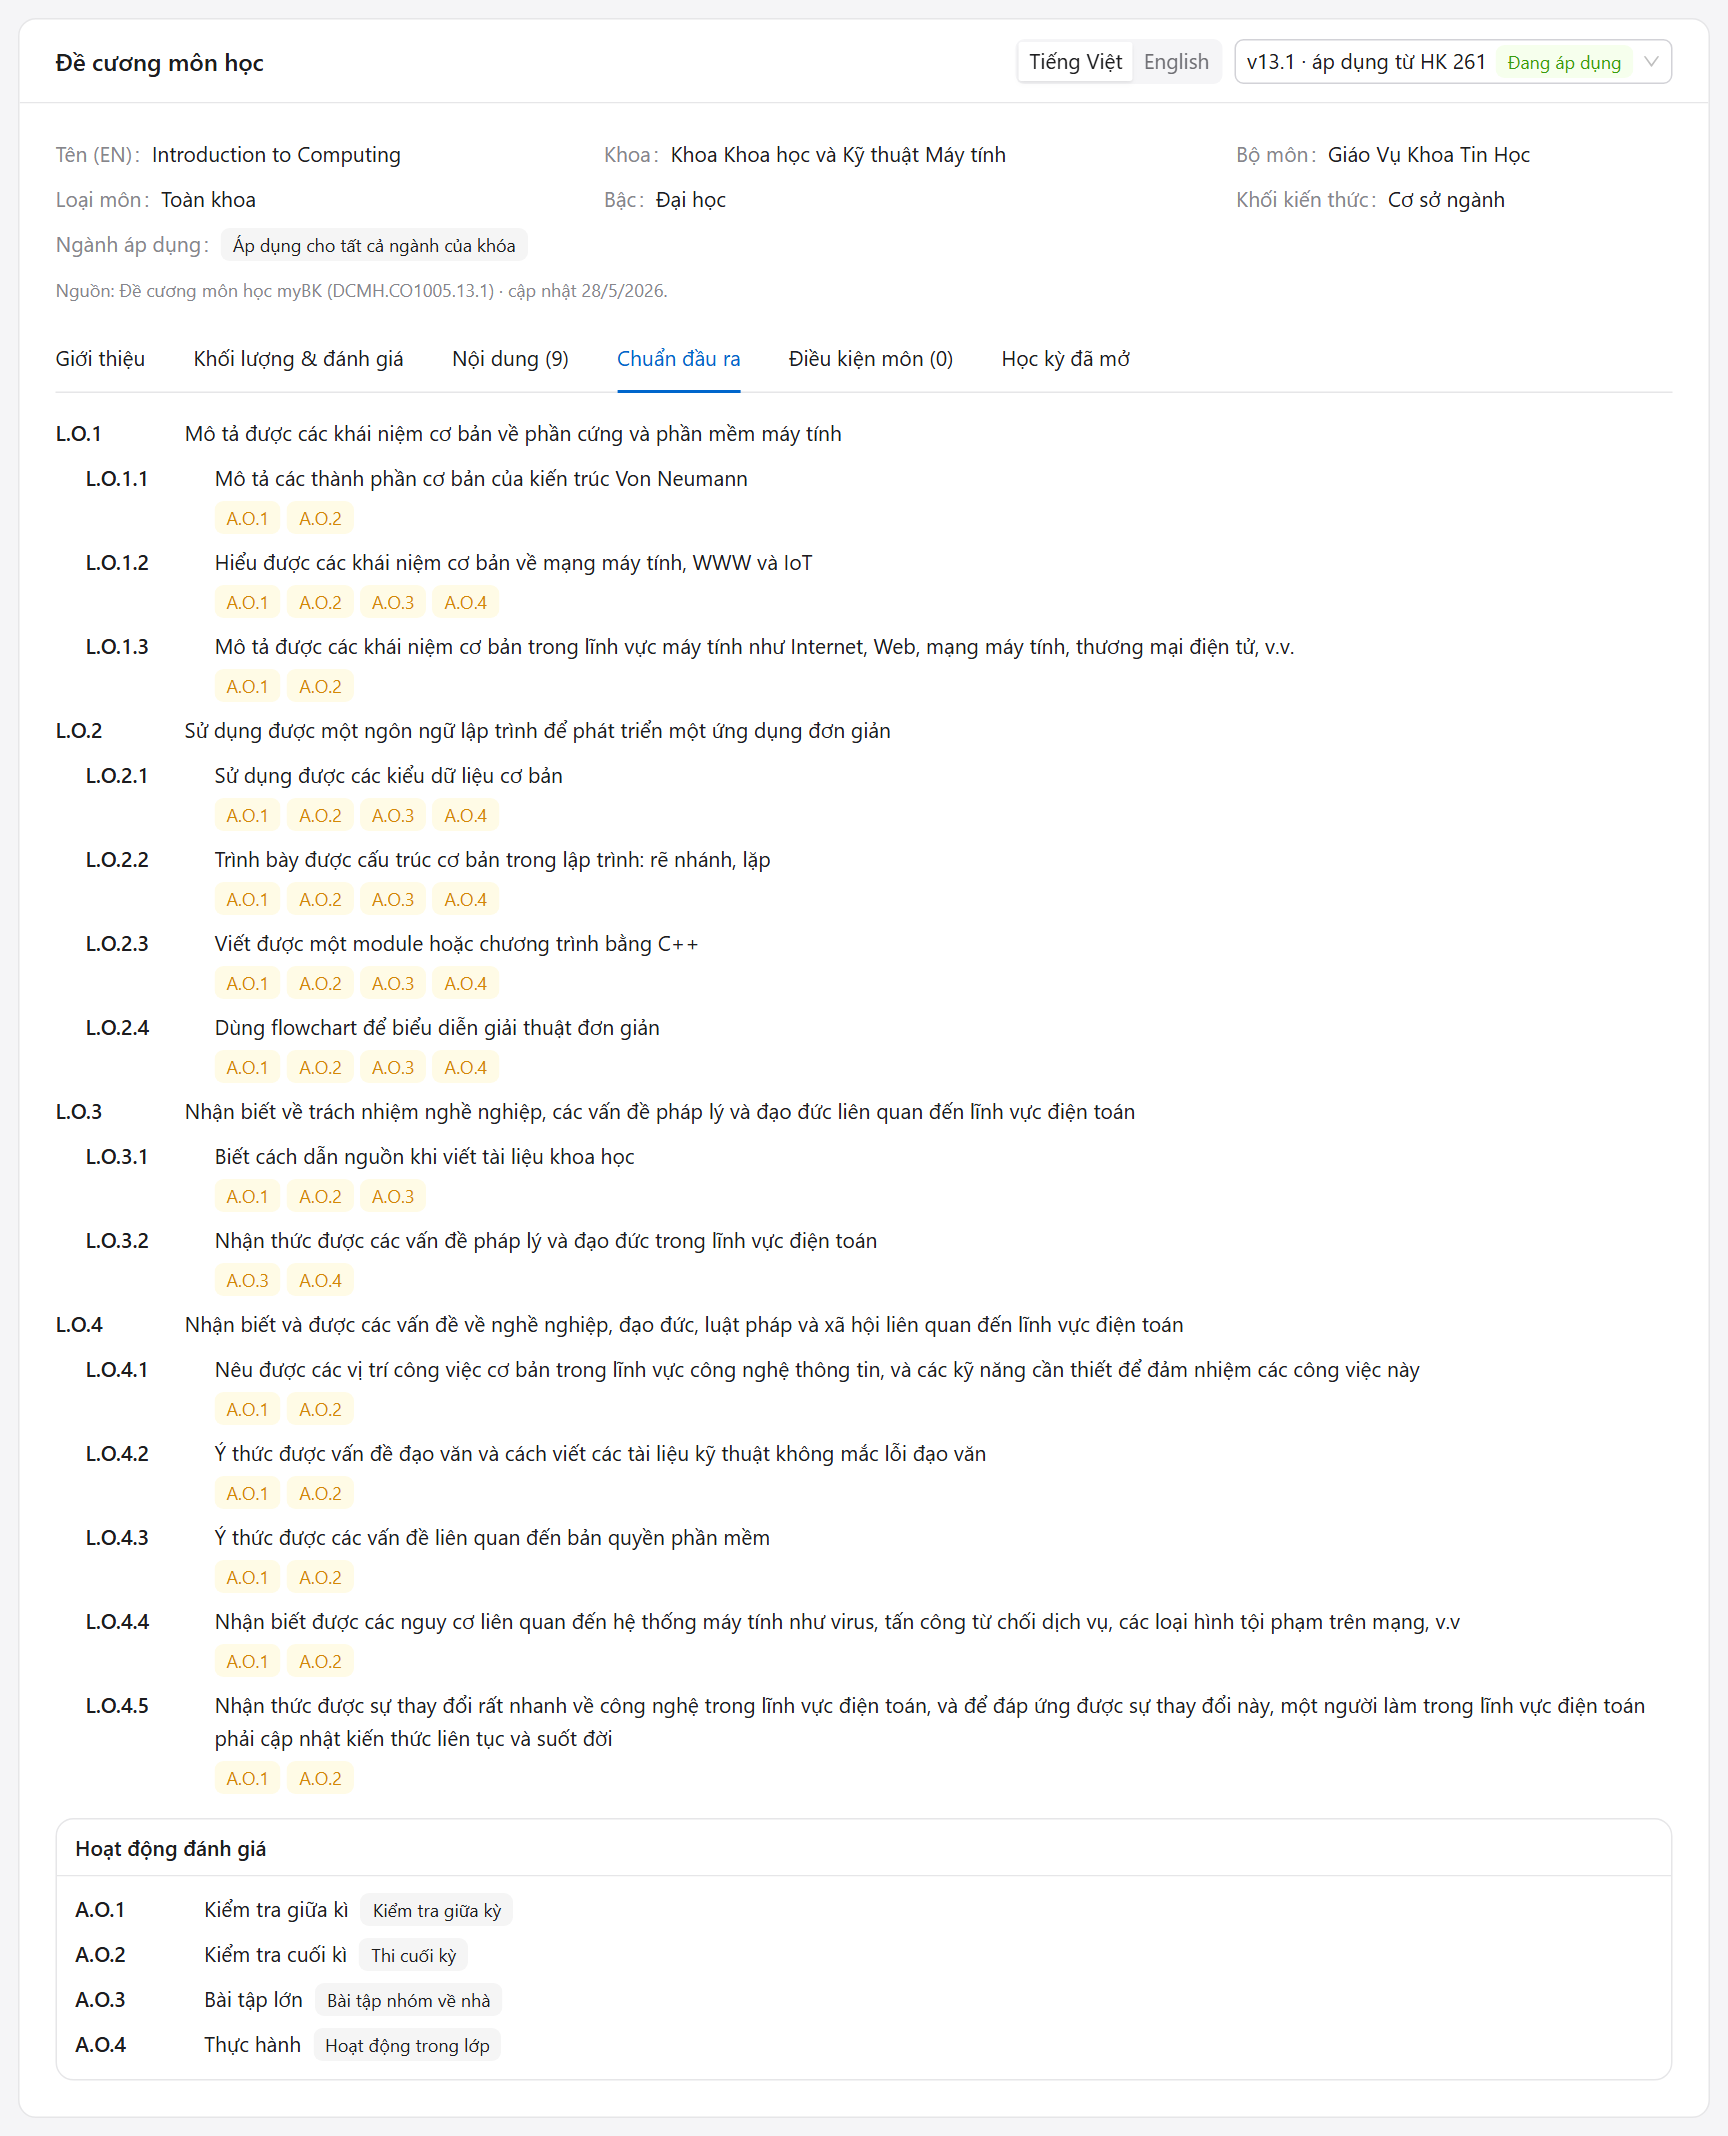
\includegraphics[width=0.9\textwidth,height=0.75\textheight,keepaspectratio]{image/ui/detail-outcomes.png}
    \caption{The Learning Outcomes tab}
    \label{fig:ui-detail-outcomes}
\end{figure}

Finally, the \emph{Học kỳ đã mở} (Opened Semesters) tab, shown in Figure~\ref{fig:ui-detail-opened}, helps students predict whether a course will be offered in the coming semesters. The history is drawn as a grid in which each row is an academic year and each column is a term (first term, second term and summer term). Each cell indicates whether the course was opened, not opened, or has not yet taken place, and the current semester is highlighted with a dark border. Below the grid, a frequency bar summarizes how often the course was opened in each term, followed by a short conclusion in plain language.

\begin{figure}[H]
    \centering
    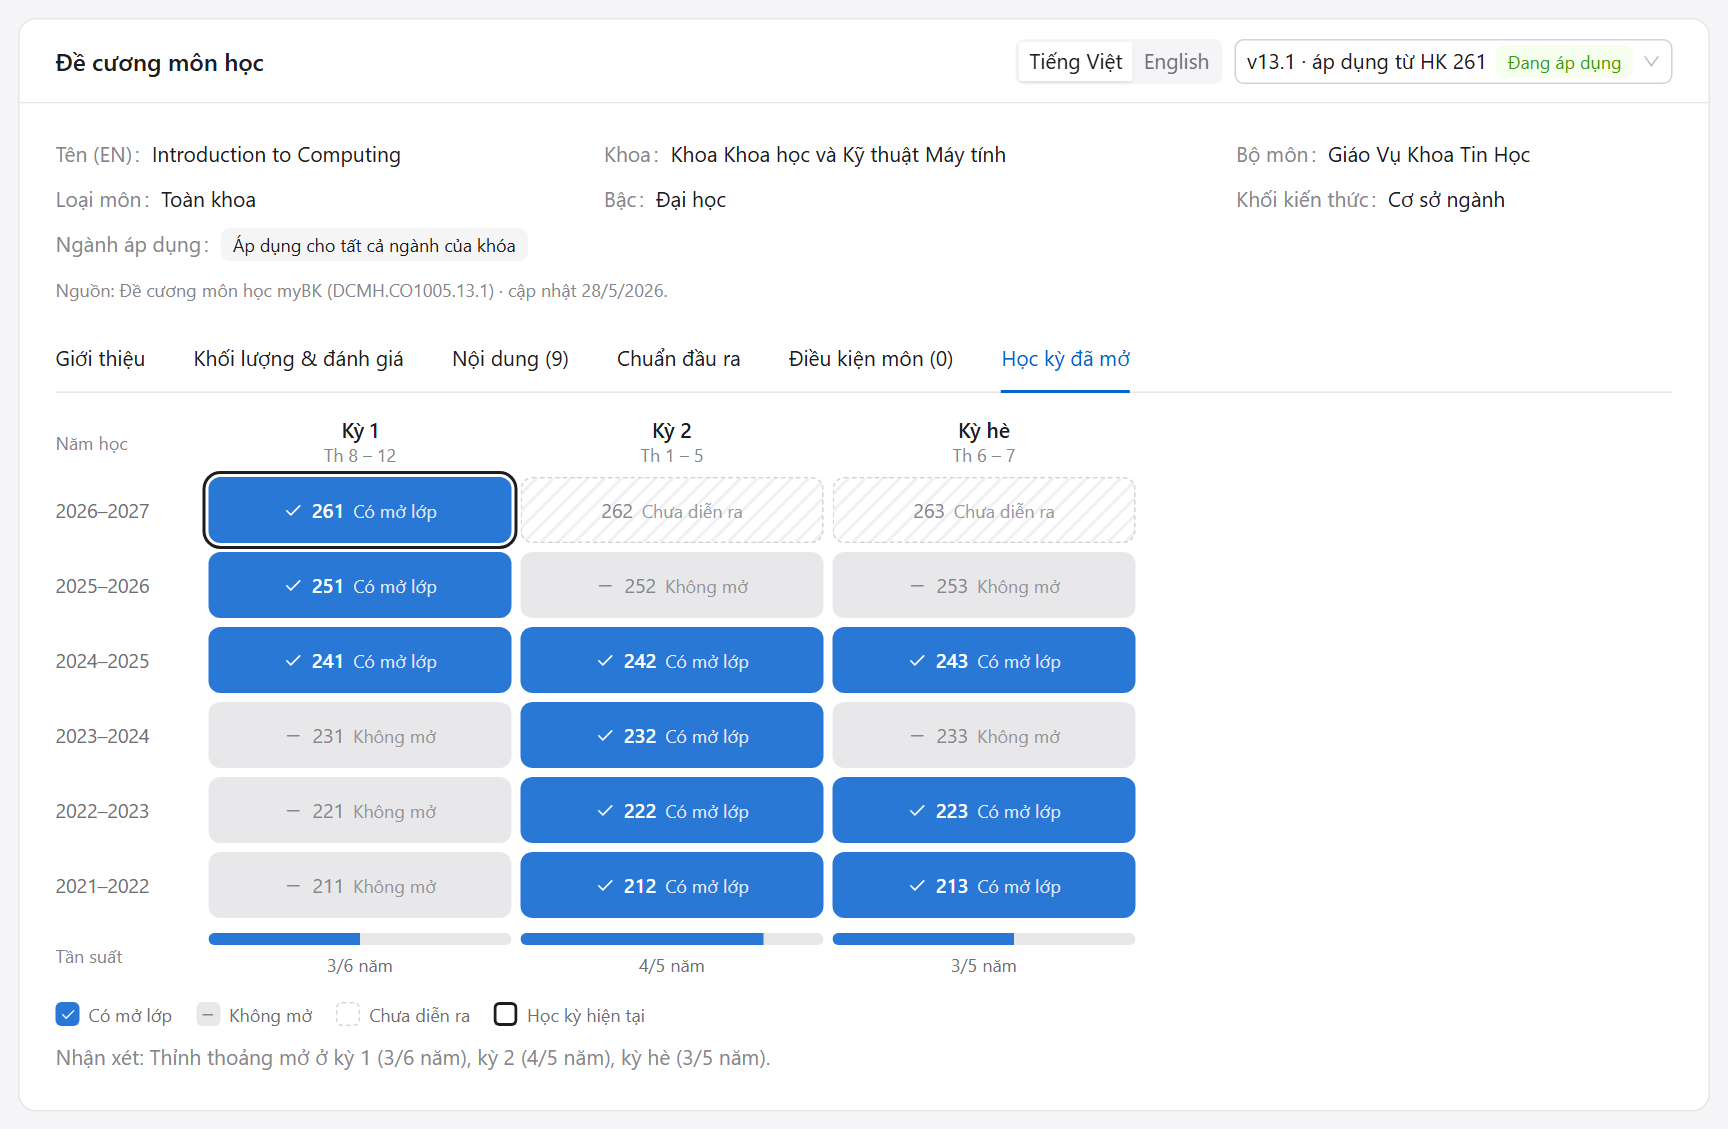
\includegraphics[width=0.9\textwidth]{image/ui/detail-opened.png}
    \caption{The Opened Semesters tab}
    \label{fig:ui-detail-opened}
\end{figure}

\subsubsection{Learning Analysis Page}
\label{subsubsec:ui-analysis}

From the Course List page, students can open the \emph{Phân tích học tập} (Learning Analysis) page, which combines the curriculum, the declared course statuses and the study plan to evaluate the student's progress towards graduation. The subtitle of the page states exactly which curriculum and which semester the analysis is based on, as well as how many courses have an outline available. The content of the page is organized into a series of cards, each answering one question about the student's progress; the main ones are presented below.

At the top of the page, the overview card shown in Figure~\ref{fig:ui-analysis-overview} answers the question of how far the student is from graduation. A ring chart shows the percentage of graduation credits earned, next to the number of earned credits over the required credits and the number of courses counted towards graduation. On the right are the key figures: credits in progress, credits planned, credits still missing, the average number of credits completed per semester so far, the number of credits per semester required to graduate on time, and the projected graduation semester compared with the standard one. A stacked bar at the bottom of the card splits the graduation credits into completed, in-progress, planned and missing parts.

\begin{figure}[H]
    \centering
    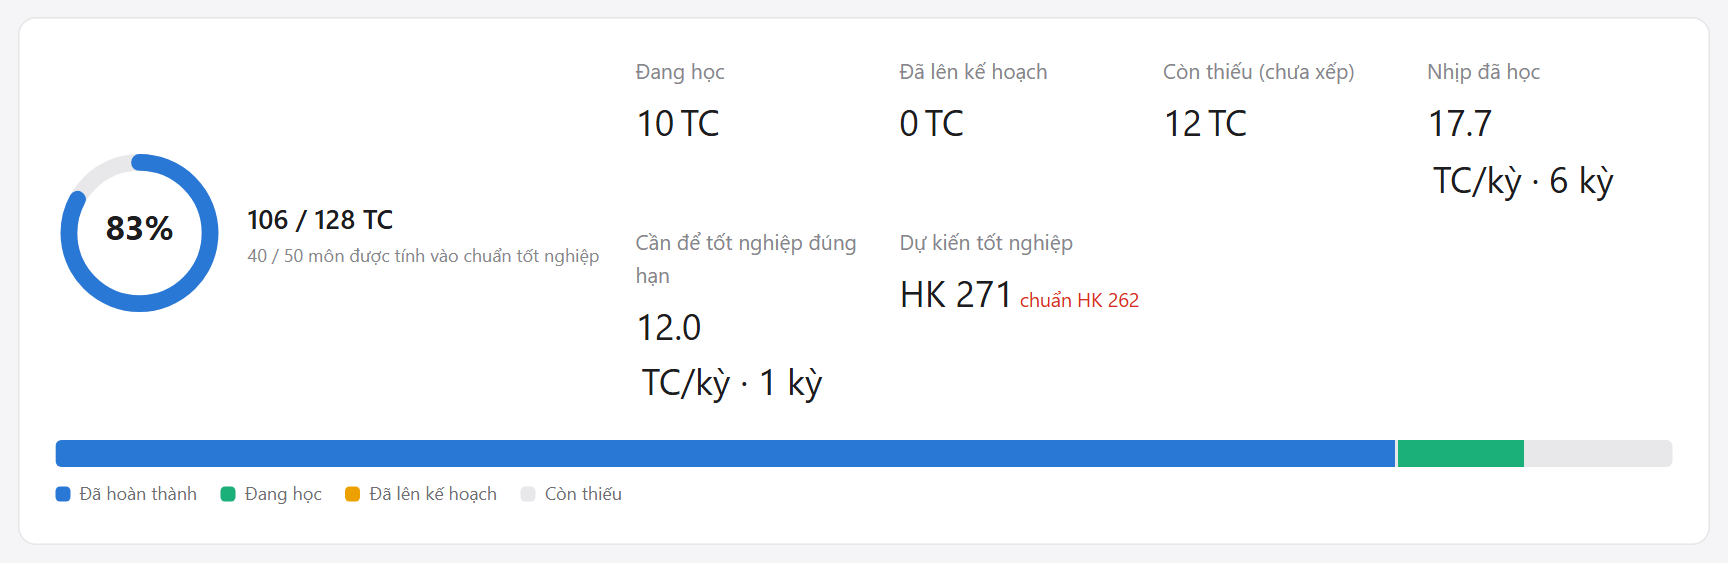
\includegraphics[width=\textwidth]{image/ui/analysis-overview.png}
    \caption{The overview card of the Learning Analysis page}
    \label{fig:ui-analysis-overview}
\end{figure}

Below the overview, two charts placed side by side break the progress down further, as shown in Figure~\ref{fig:ui-analysis-progress}. On the left, \emph{Tiến độ theo khối kiến thức} (Progress by knowledge block) shows one progress bar for the required courses and for each elective group, together with the number of courses that must be chosen in the group. On the right, \emph{Theo khung chương trình (môn bắt buộc)} (By curriculum framework, required courses) is a column chart in which each column is a semester of the standard framework, mapped to the actual semester according to the admission year. The column of the current semester is highlighted with a background, and grey parts in the earlier columns reveal required courses that the student is behind on.

\begin{figure}[H]
    \centering
    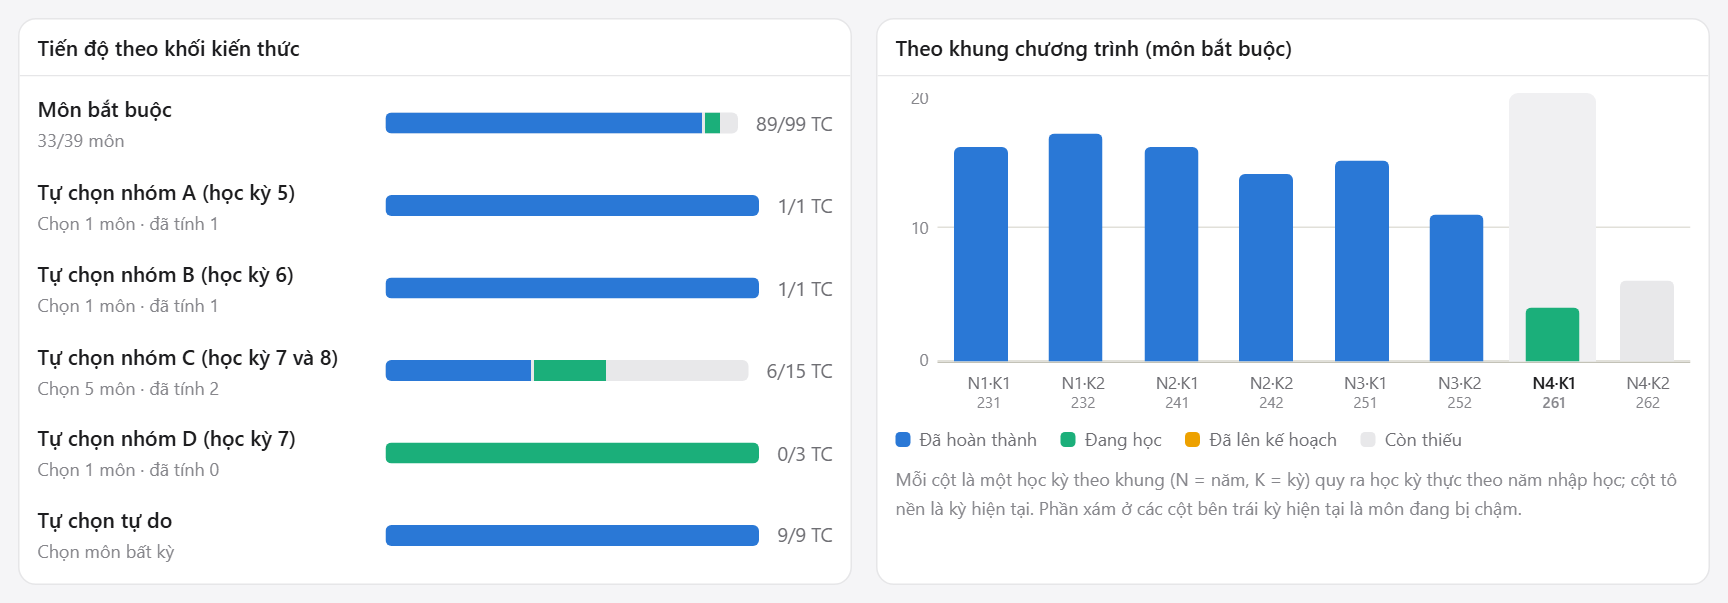
\includegraphics[width=\textwidth]{image/ui/analysis-progress.png}
    \caption{Progress by knowledge block and by curriculum framework}
    \label{fig:ui-analysis-progress}
\end{figure}

The \emph{Môn còn thiếu} (Missing courses) card, shown in Figure~\ref{fig:ui-analysis-missing}, lists the courses that the student still has to complete, grouped into four tabs: required courses whose recommended semester has already passed, the remaining required courses, the elective groups that still lack courses, and the courses that the student has failed. The figure shows the \emph{Bắt buộc còn lại} (Remaining required courses) tab, which contains four courses for the demo student. Each row gives the course name together with its exam format and estimated study hours, its credits and recommended semester, whether the student meets its requirements, how often it has been opened in the next term along with the latest semester it was opened, and the student's current status. When the outline states an additional requirement that is not declared in the curriculum, such as the prerequisite \texttt{CO4359} of the capstone project \texttt{CO4337}, it is highlighted in orange next to the eligibility tag so that the student can verify it with the faculty.

\begin{figure}[H]
    \centering
    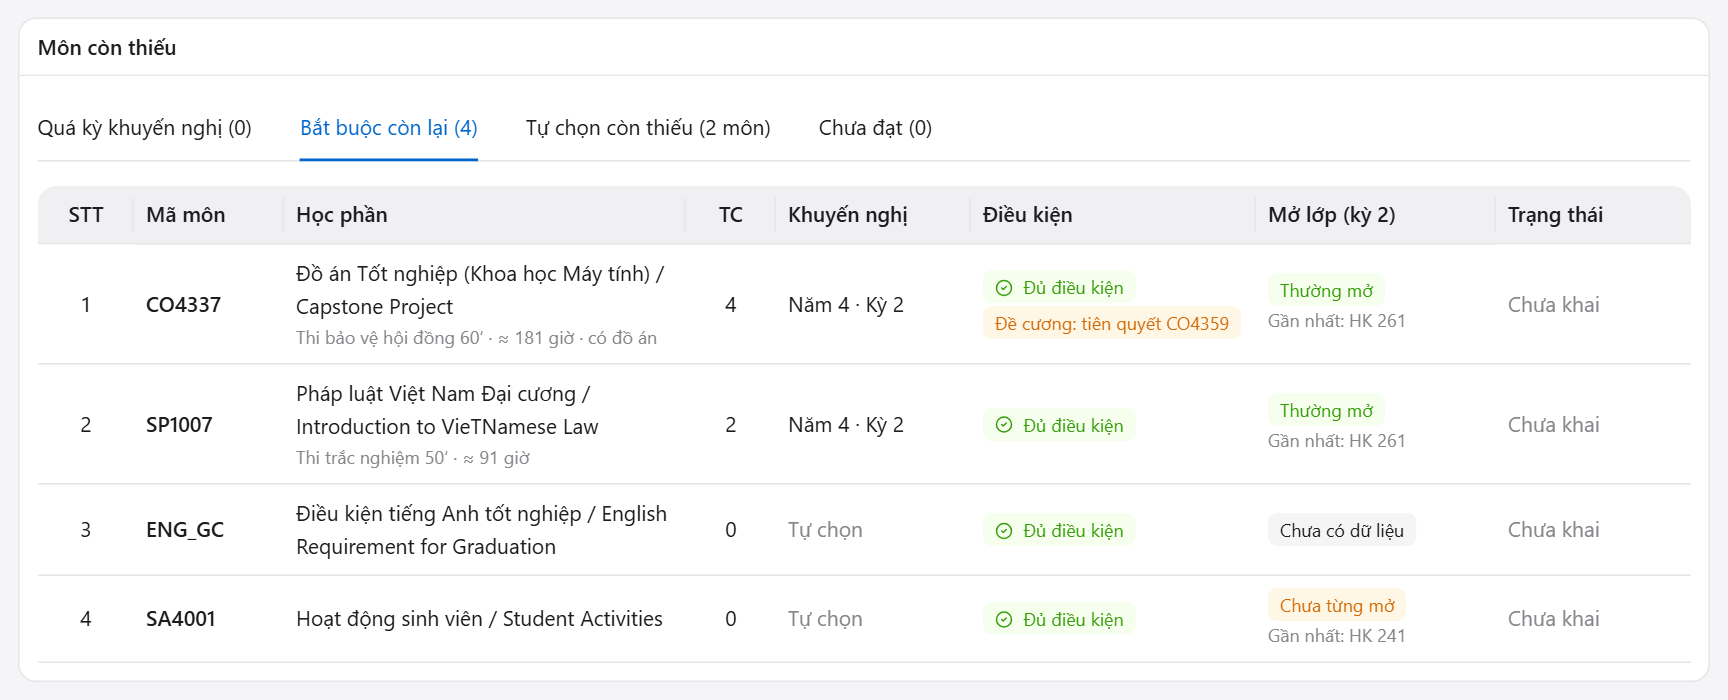
\includegraphics[width=\textwidth]{image/ui/analysis-missing.png}
    \caption{The Missing courses card}
    \label{fig:ui-analysis-missing}
\end{figure}

The \emph{Các lựa chọn} (Options) card, illustrated in Figure~\ref{fig:ui-analysis-options}, supports the student in choosing a specialization and electives. Its first part, \emph{Chuyên ngành (không bắt buộc)} (Specializations, optional), shows one progress bar per specialization, counting the courses of its list that the student has taken or is taking. Under each specialization name, a note tells the student whether the specialization is still achievable or, if not, which elective courses outside the list prevent it. The second part lists, for each elective group that is not yet complete, all candidate courses in a table with their exam format and estimated study hours, the specializations they belong to, their credits, whether the student meets their requirements, how often they are opened in the next term and the student's current status. The figure shows the beginning of the table for elective group C.

\begin{figure}[H]
    \centering
    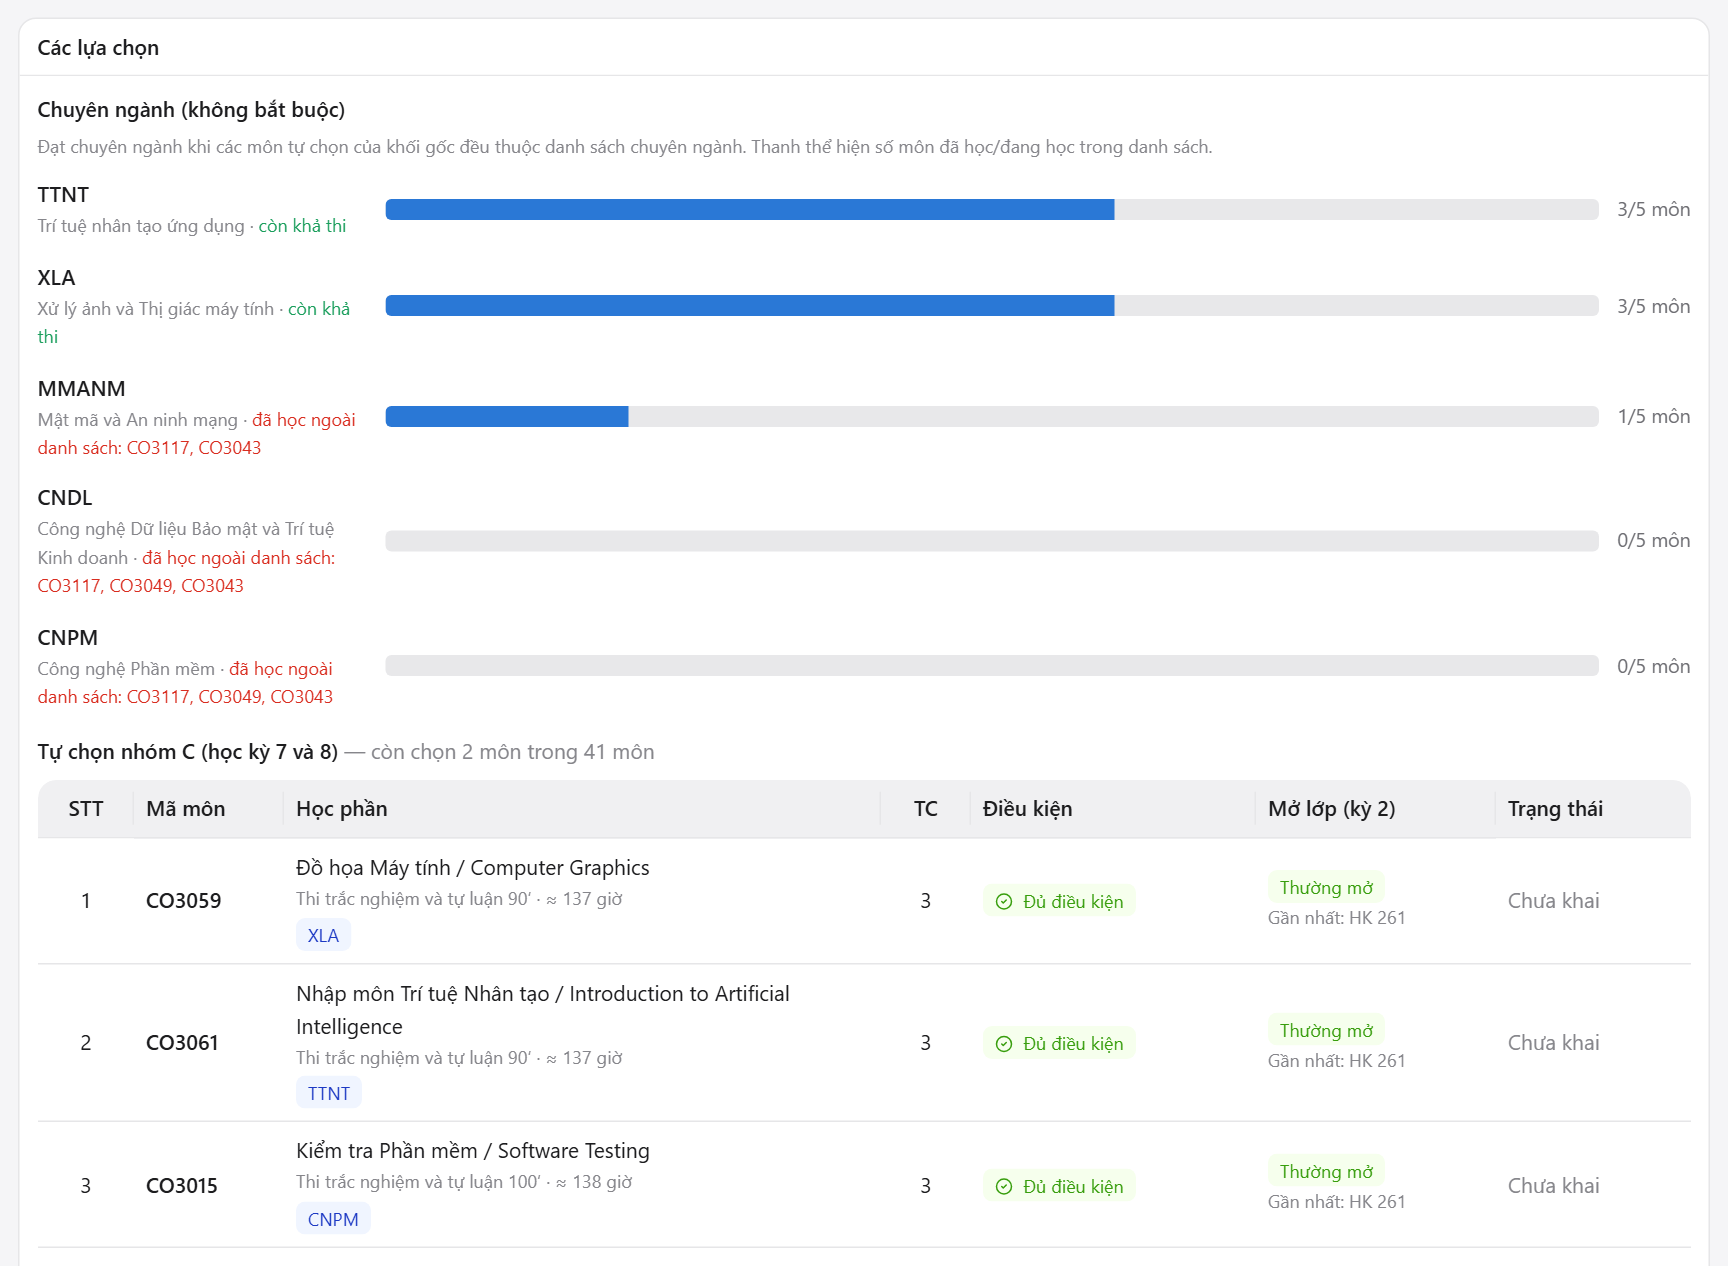
\includegraphics[width=\textwidth]{image/ui/analysis-options.png}
    \caption{The Options card with specializations and elective courses}
    \label{fig:ui-analysis-options}
\end{figure}

Further down, the page also lists the courses that can be registered in the next semester, the ``bottleneck'' courses that unlock the largest number of other courses, and a suggested roadmap to graduation. Finally, the \emph{Điều kiện tốt nghiệp khác} (Other graduation requirements) card, shown in Figure~\ref{fig:ui-analysis-regulations}, reminds the student of the graduation requirements that are not courses, such as the English proficiency requirement and student activities. Each requirement is displayed with an icon indicating whether it has been fulfilled, and the \emph{Cập nhật} (Update) link leads to the graduation regulations page, where the student can update their status.

\begin{figure}[H]
    \centering
    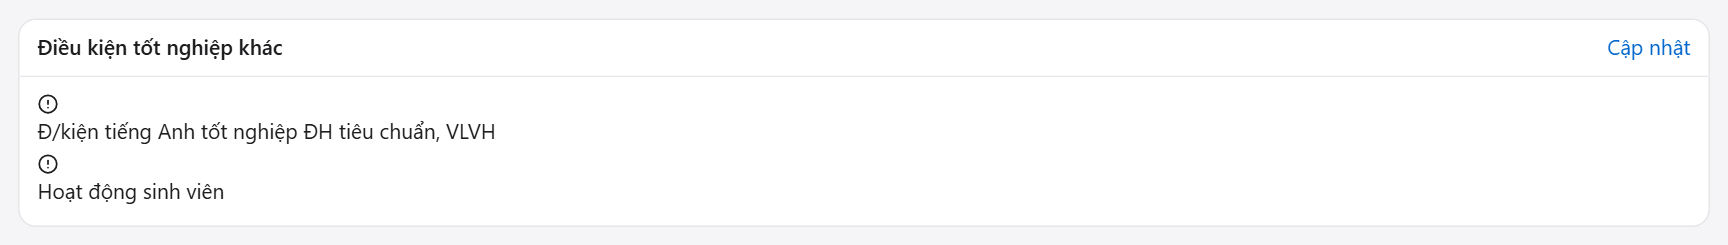
\includegraphics[width=\textwidth]{image/ui/analysis-regulations.png}
    \caption{The Other graduation requirements card}
    \label{fig:ui-analysis-regulations}
\end{figure}

\subsubsection{AI Advisor Page}
\label{subsubsec:ui-advisor}

For questions that cannot be answered by the analysis alone, such as which elective suits the student's interests, students can turn to the \emph{Tư vấn với AI} (AI Advisor) page. The subtitle reminds students that the advisor relies on the result of the Learning Analysis at the current semester, gives suggestions for the next one, and may be wrong. The header also contains a selector of previous conversations, a \emph{Mới} (New) button to start a new conversation and a \emph{Xóa} (Delete) button. The content area has two tabs: \emph{Trò chuyện} (Chat) and \emph{Trajectory}.

When a new conversation is started, the Chat tab shows a short introduction explaining what the advisor can do, together with several suggested questions so that students can start with one click, as shown in Figure~\ref{fig:ui-advisor-empty}. Questions can also be typed into the input box at the bottom of the page.

\begin{figure}[H]
    \centering
    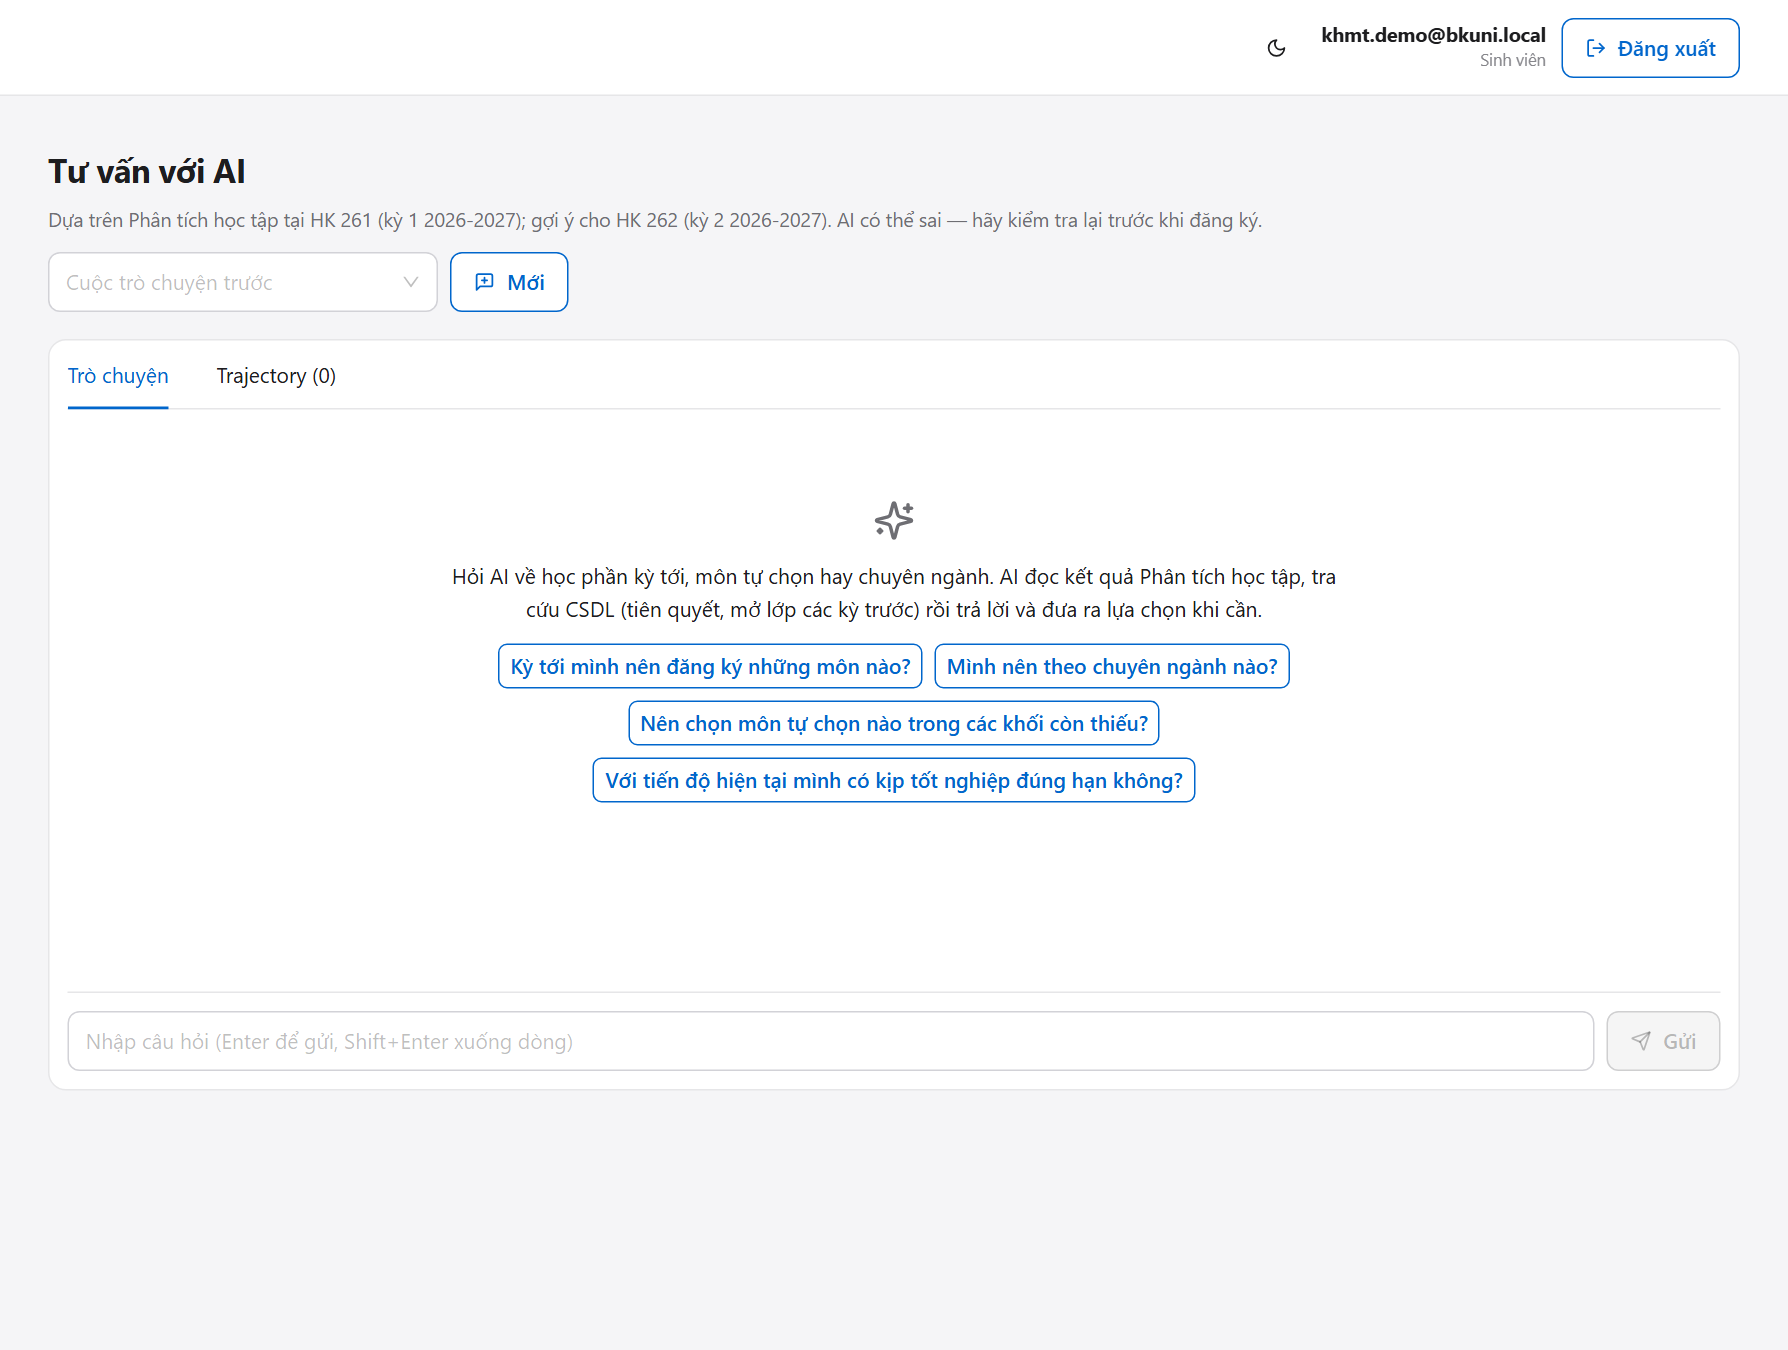
\includegraphics[width=\textwidth]{image/ui/advisor-empty.png}
    \caption{The AI Advisor page when starting a new conversation}
    \label{fig:ui-advisor-empty}
\end{figure}

After a question is sent, the advisor reads the analysis, queries the database through its tools and replies in the chat thread, as illustrated in Figure~\ref{fig:ui-advisor-chat}. The student's question appears on the right and the answer on the left. Besides the written explanation, the answer contains a list of suggested courses, each displayed as a card with its priority, the reason for the suggestion, a summary of its outline (exam format and estimated study hours), and tags indicating whether the student meets its requirements and how likely it is to be offered next semester.

\begin{figure}[H]
    \centering
    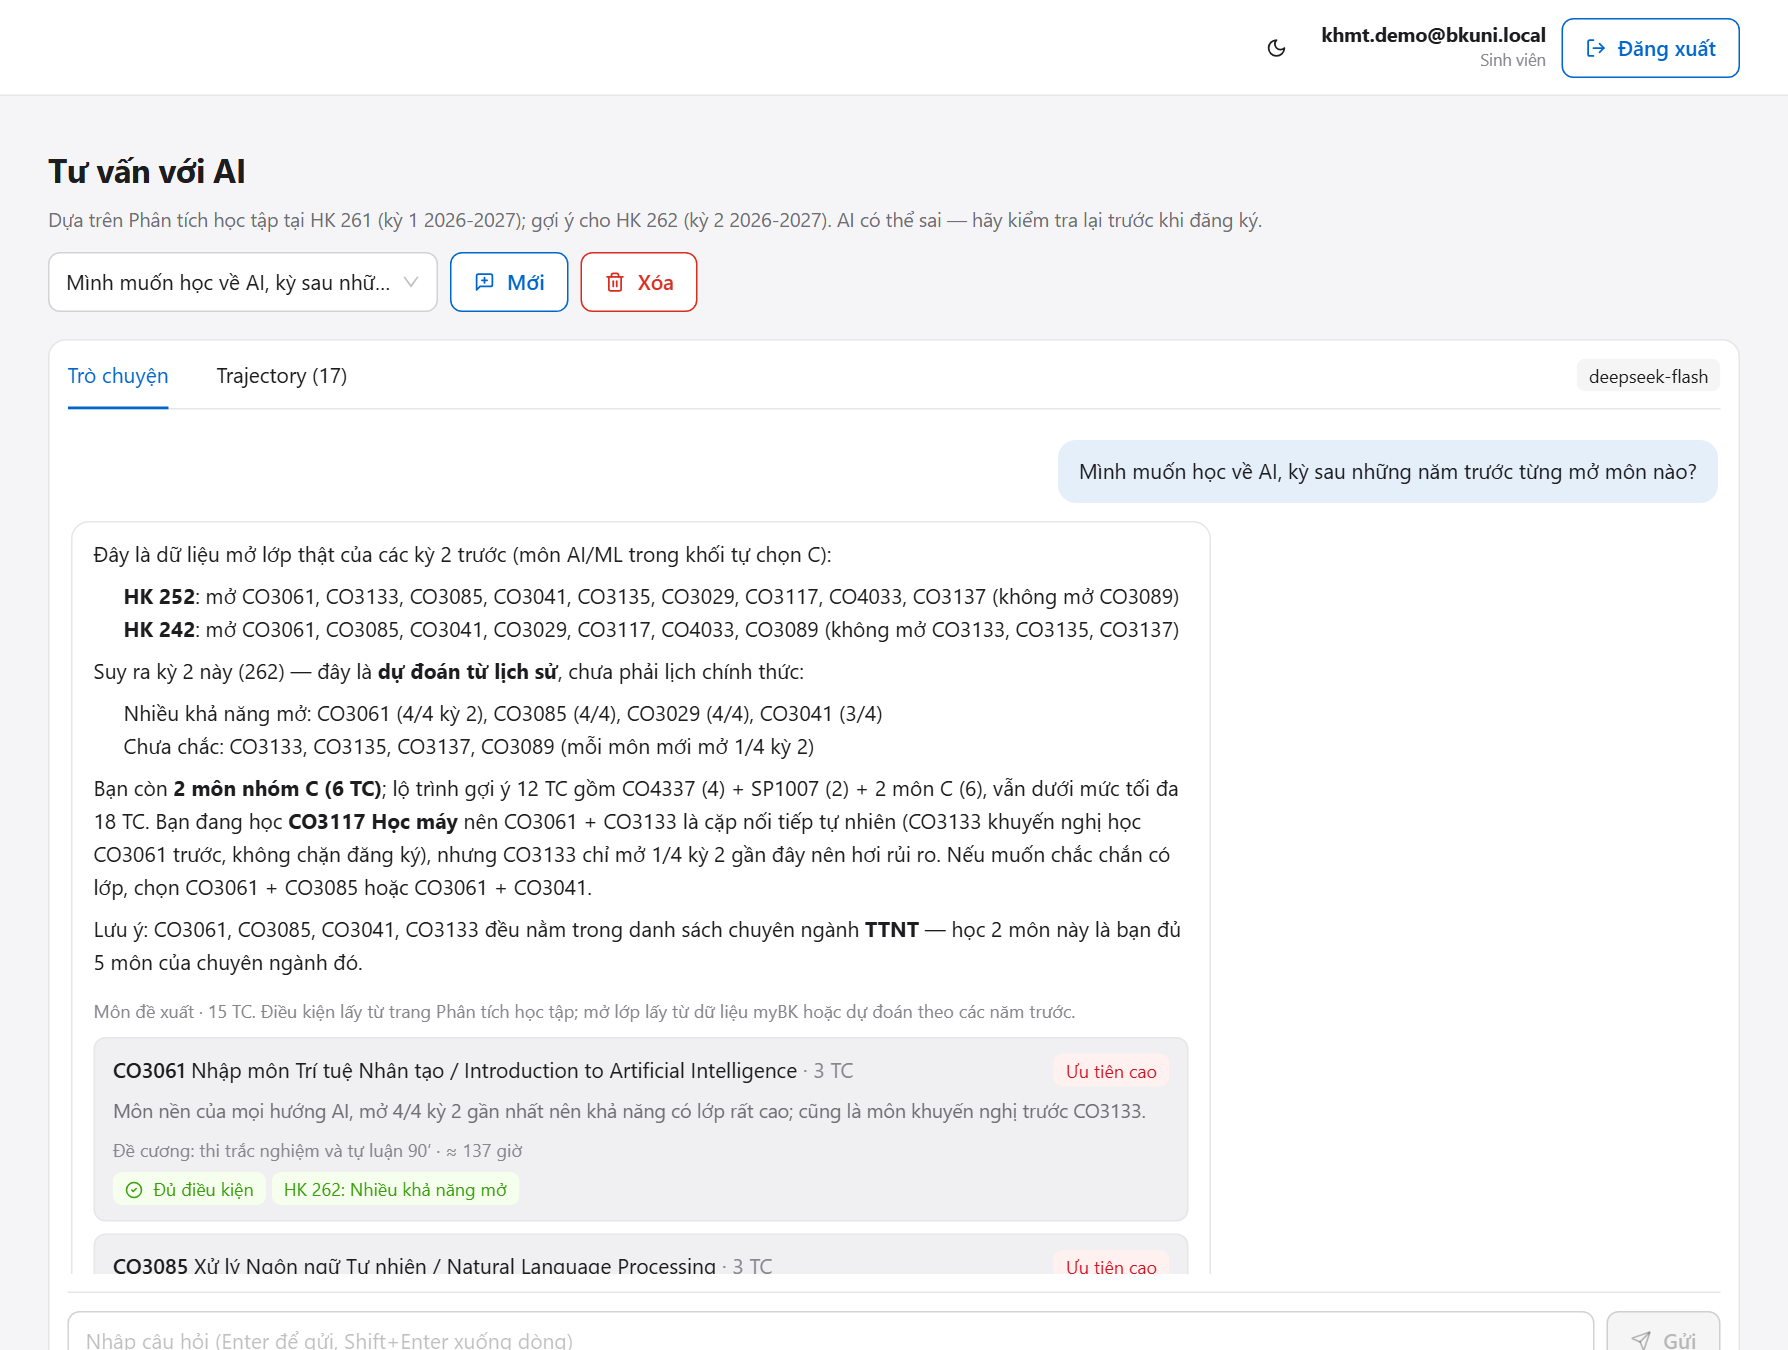
\includegraphics[width=\textwidth]{image/ui/advisor-chat-top.png}
    \caption{An answer of the AI advisor with suggested courses}
    \label{fig:ui-advisor-chat}
\end{figure}

When the advisor needs more information to give a better answer, it asks the student clarifying questions with predefined options instead of guessing, as shown in Figure~\ref{fig:ui-advisor-choices}. Each option comes with a short explanation, and an additional text box lets the student give a different answer before clicking \emph{Gửi lựa chọn} (Send choices). Follow-up questions are also suggested at the end of the answer so that the conversation can continue naturally.

\begin{figure}[H]
    \centering
    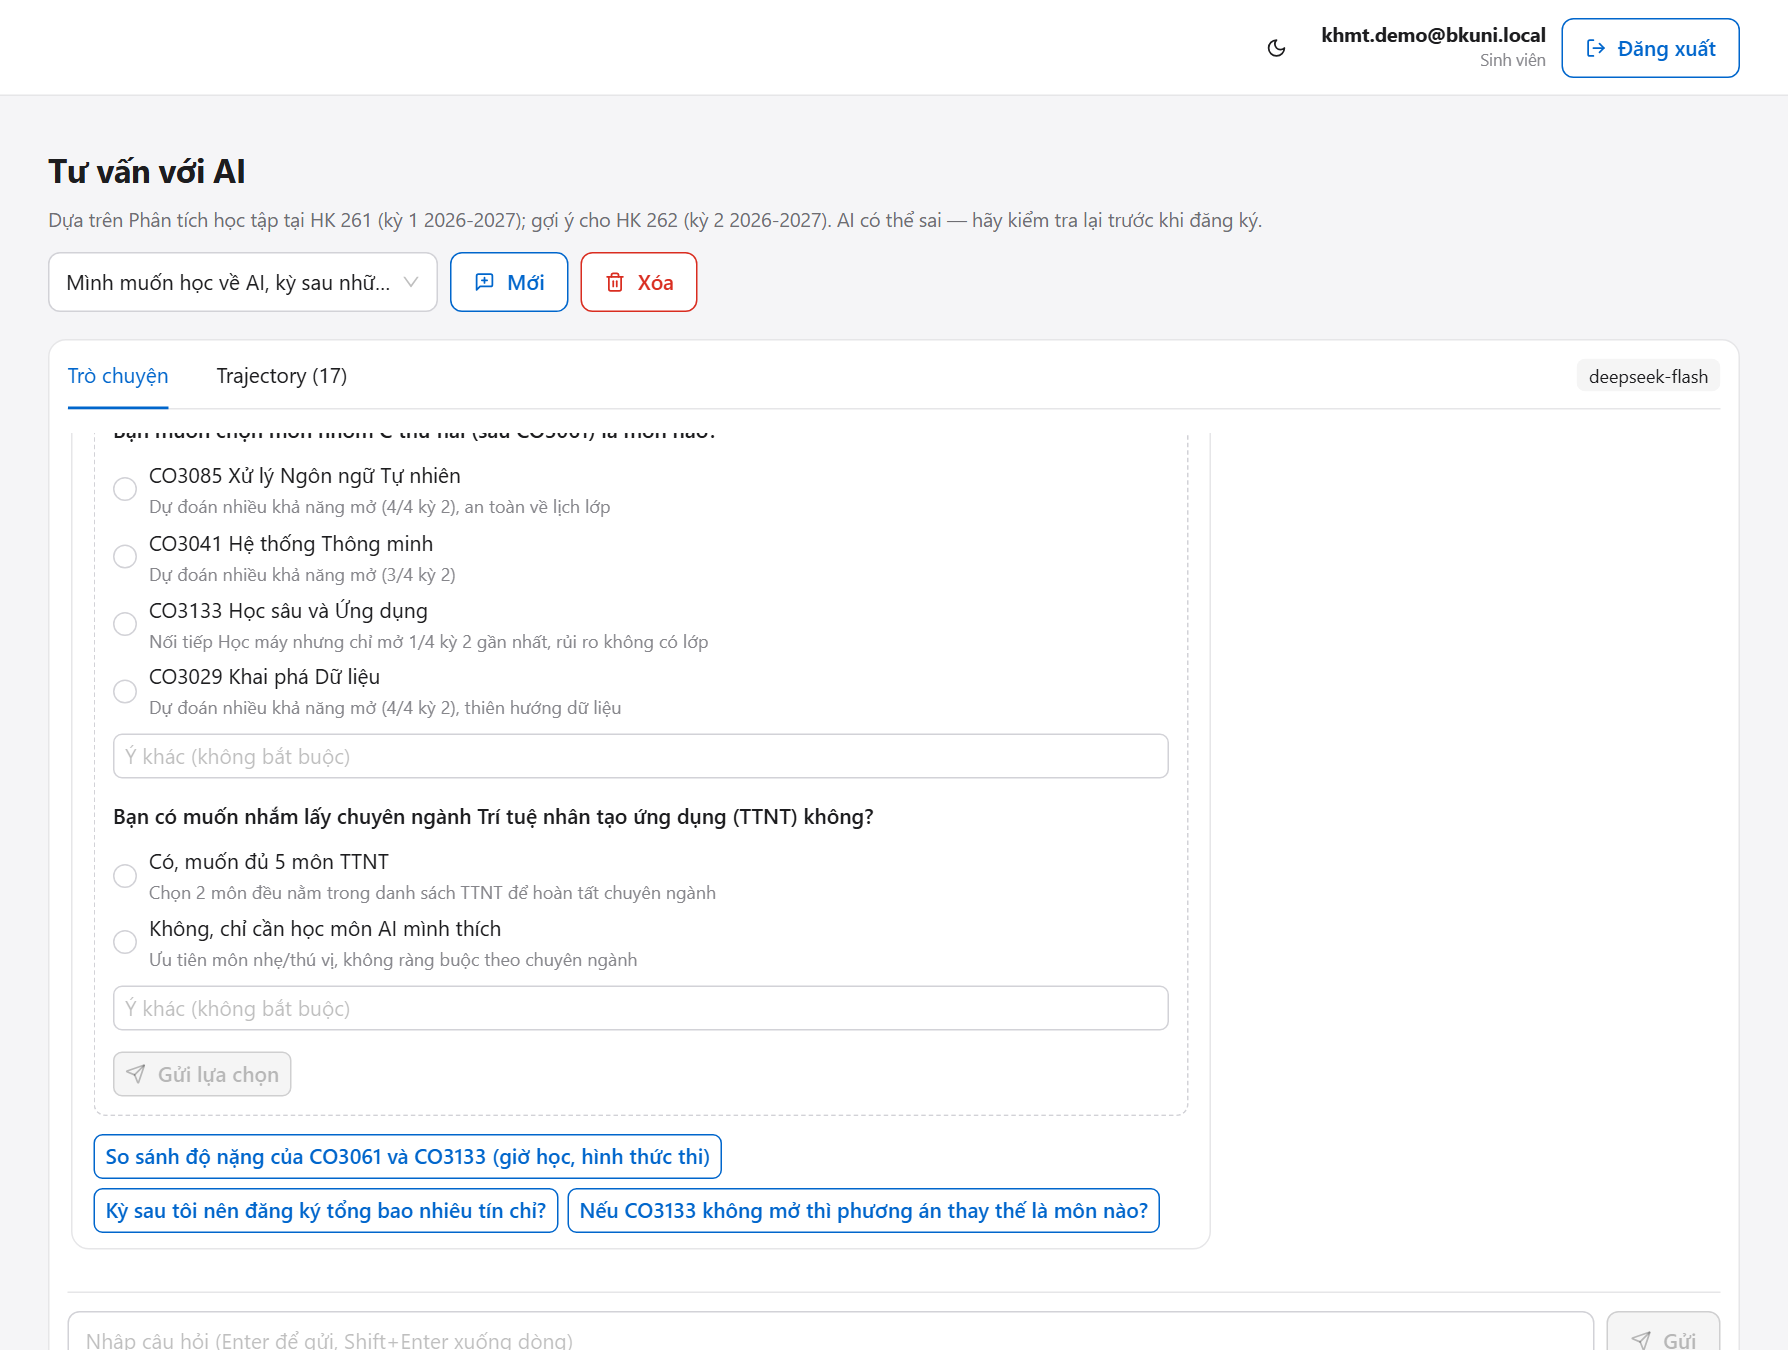
\includegraphics[width=\textwidth]{image/ui/advisor-chat-bottom.png}
    \caption{Clarifying questions and follow-up suggestions in the Chat tab}
    \label{fig:ui-advisor-choices}
\end{figure}

To make the advisor transparent and easy to verify, the Trajectory tab, shown in Figure~\ref{fig:ui-advisor-trace}, records every step the agent performed to produce its answers. The steps are grouped by turn and labelled by their role: the system prompt, the analysis context, the user's message, the model's reasoning together with the tools it decided to call, each tool call with its arguments and result, and the final answer. Each row can be expanded to show its full content, and the token usage, cache hits and duration of each step are displayed on the right. A summary at the top shows the number of turns, requests, tool calls, total tokens and the cache-hit rate, and the steps can be filtered to show only model or tool steps.

\begin{figure}[H]
    \centering
    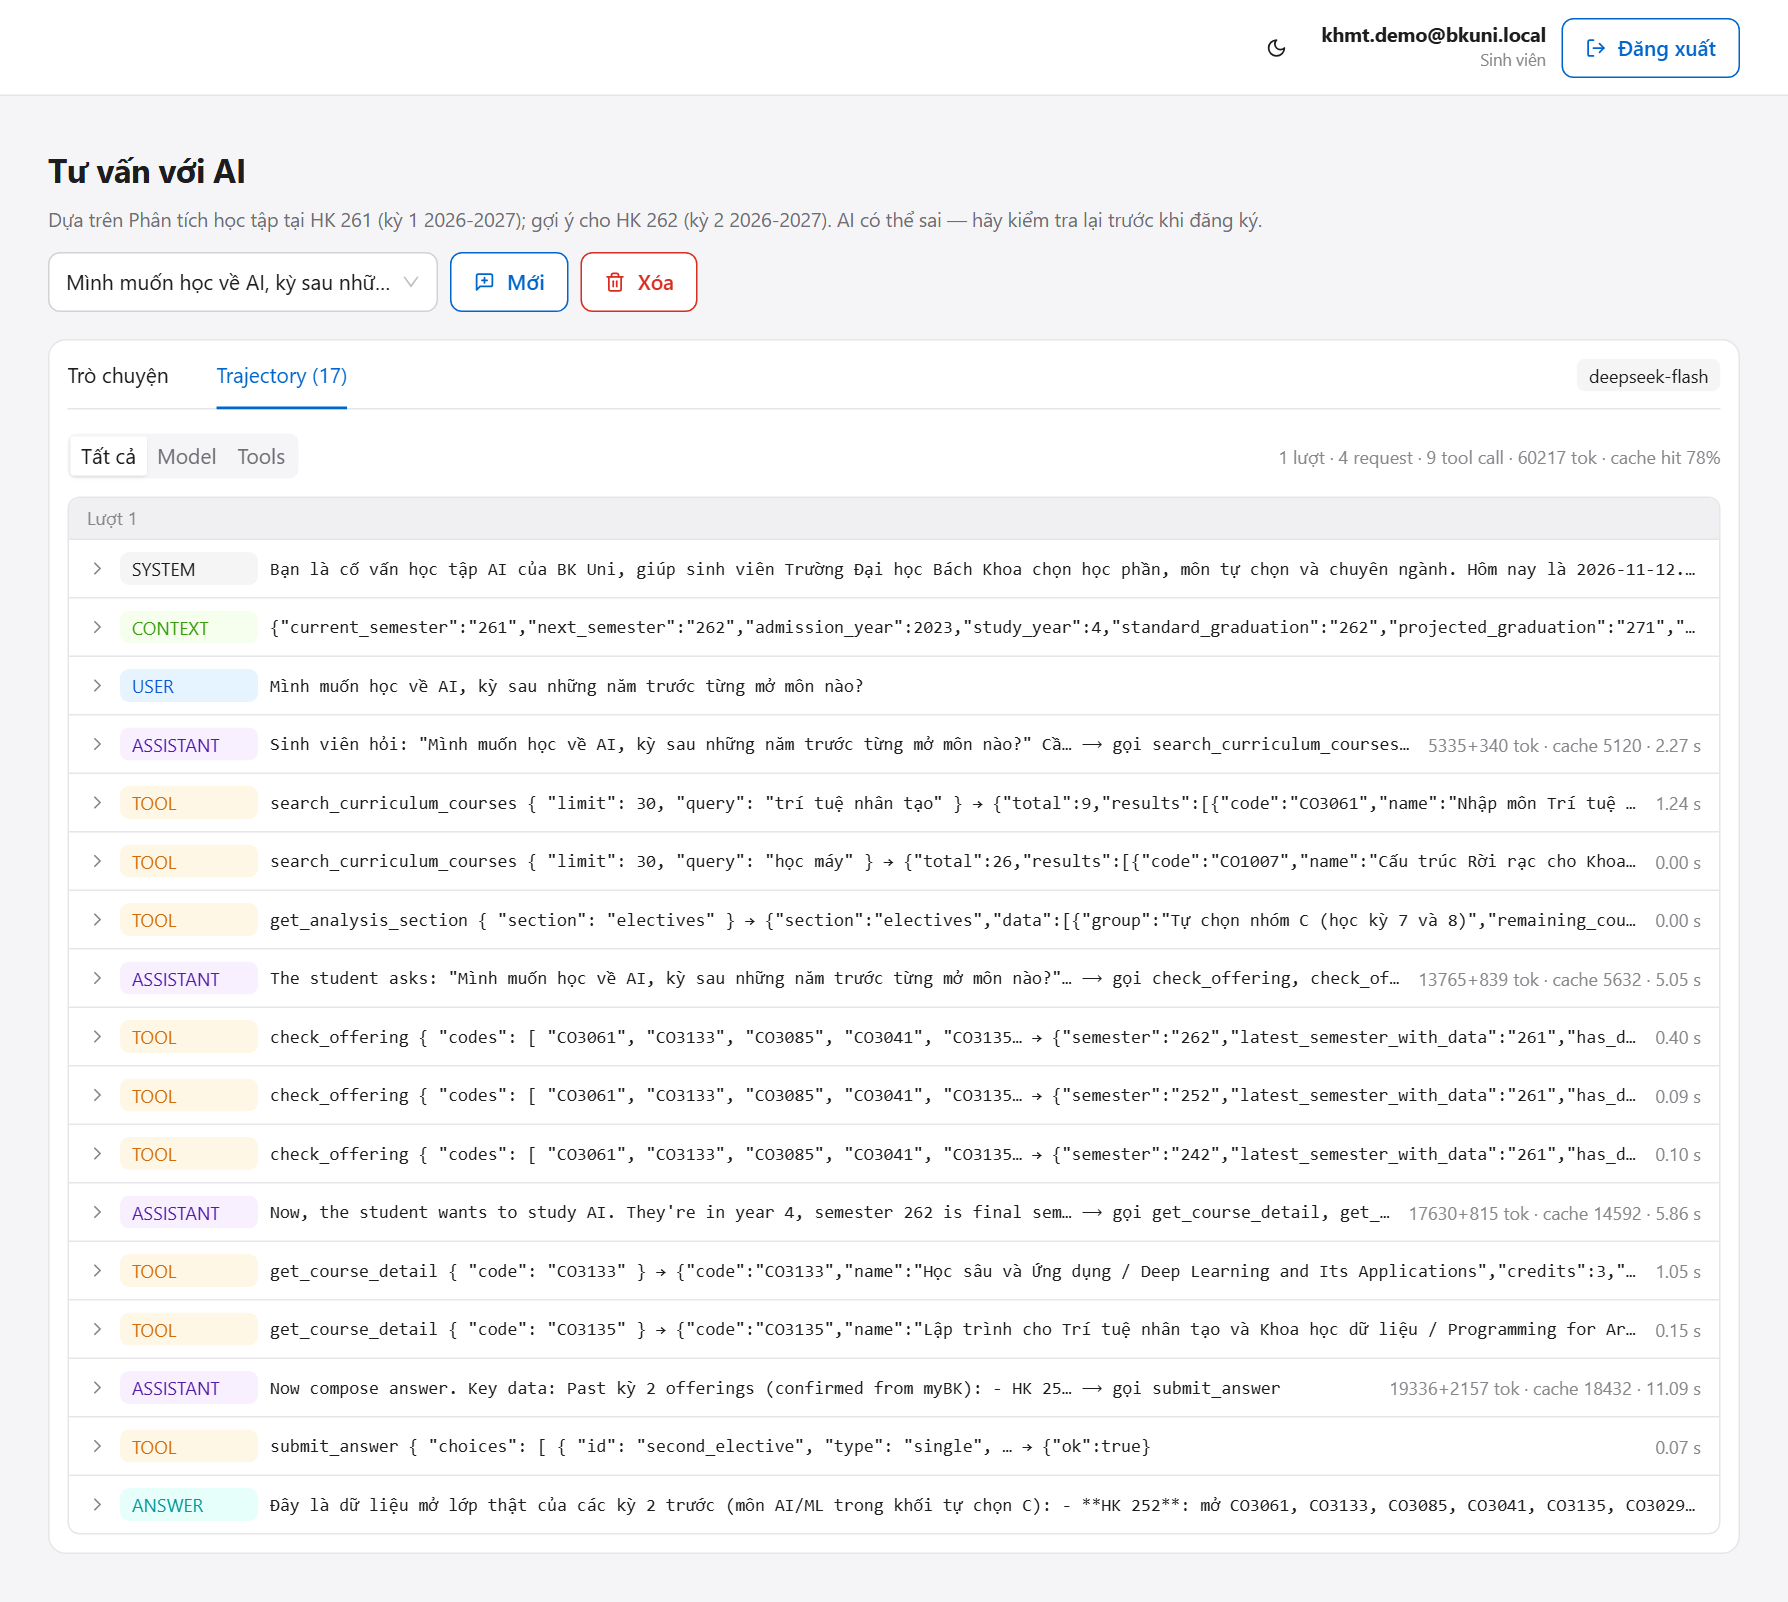
\includegraphics[width=\textwidth]{image/ui/advisor-trace.png}
    \caption{The Trajectory tab of the AI Advisor}
    \label{fig:ui-advisor-trace}
\end{figure}

\subsubsection{Personal Profile Page}
\label{subsubsec:ui-profile}

Lastly, the \emph{Hồ sơ cá nhân} (Personal Profile) page, shown in Figure~\ref{fig:ui-profile}, lets students keep their information up to date. The page consists of three cards. The \emph{Tài khoản đăng nhập} (Sign-in account) card shows the email and role of the account. The \emph{Thông tin sinh viên} (Student information) card is a form containing the full name, student number, phone number, date of birth, admission year, credit target, curriculum and contact address; short hints under the fields explain their constraints, such as the uniqueness of the student number. Among these fields, the curriculum, admission year and credit target are especially important, since they determine the courses shown on the Course List page, the semester used in the Learning Analysis and the number of credits placed in each semester of the suggested roadmap. Finally, the \emph{Chương trình đang theo học} (Current curriculum) card summarizes the selected curriculum, including its code, name, major, faculty, cohort and credit limits per semester, with a shortcut to start planning.

\begin{figure}[H]
    \centering
    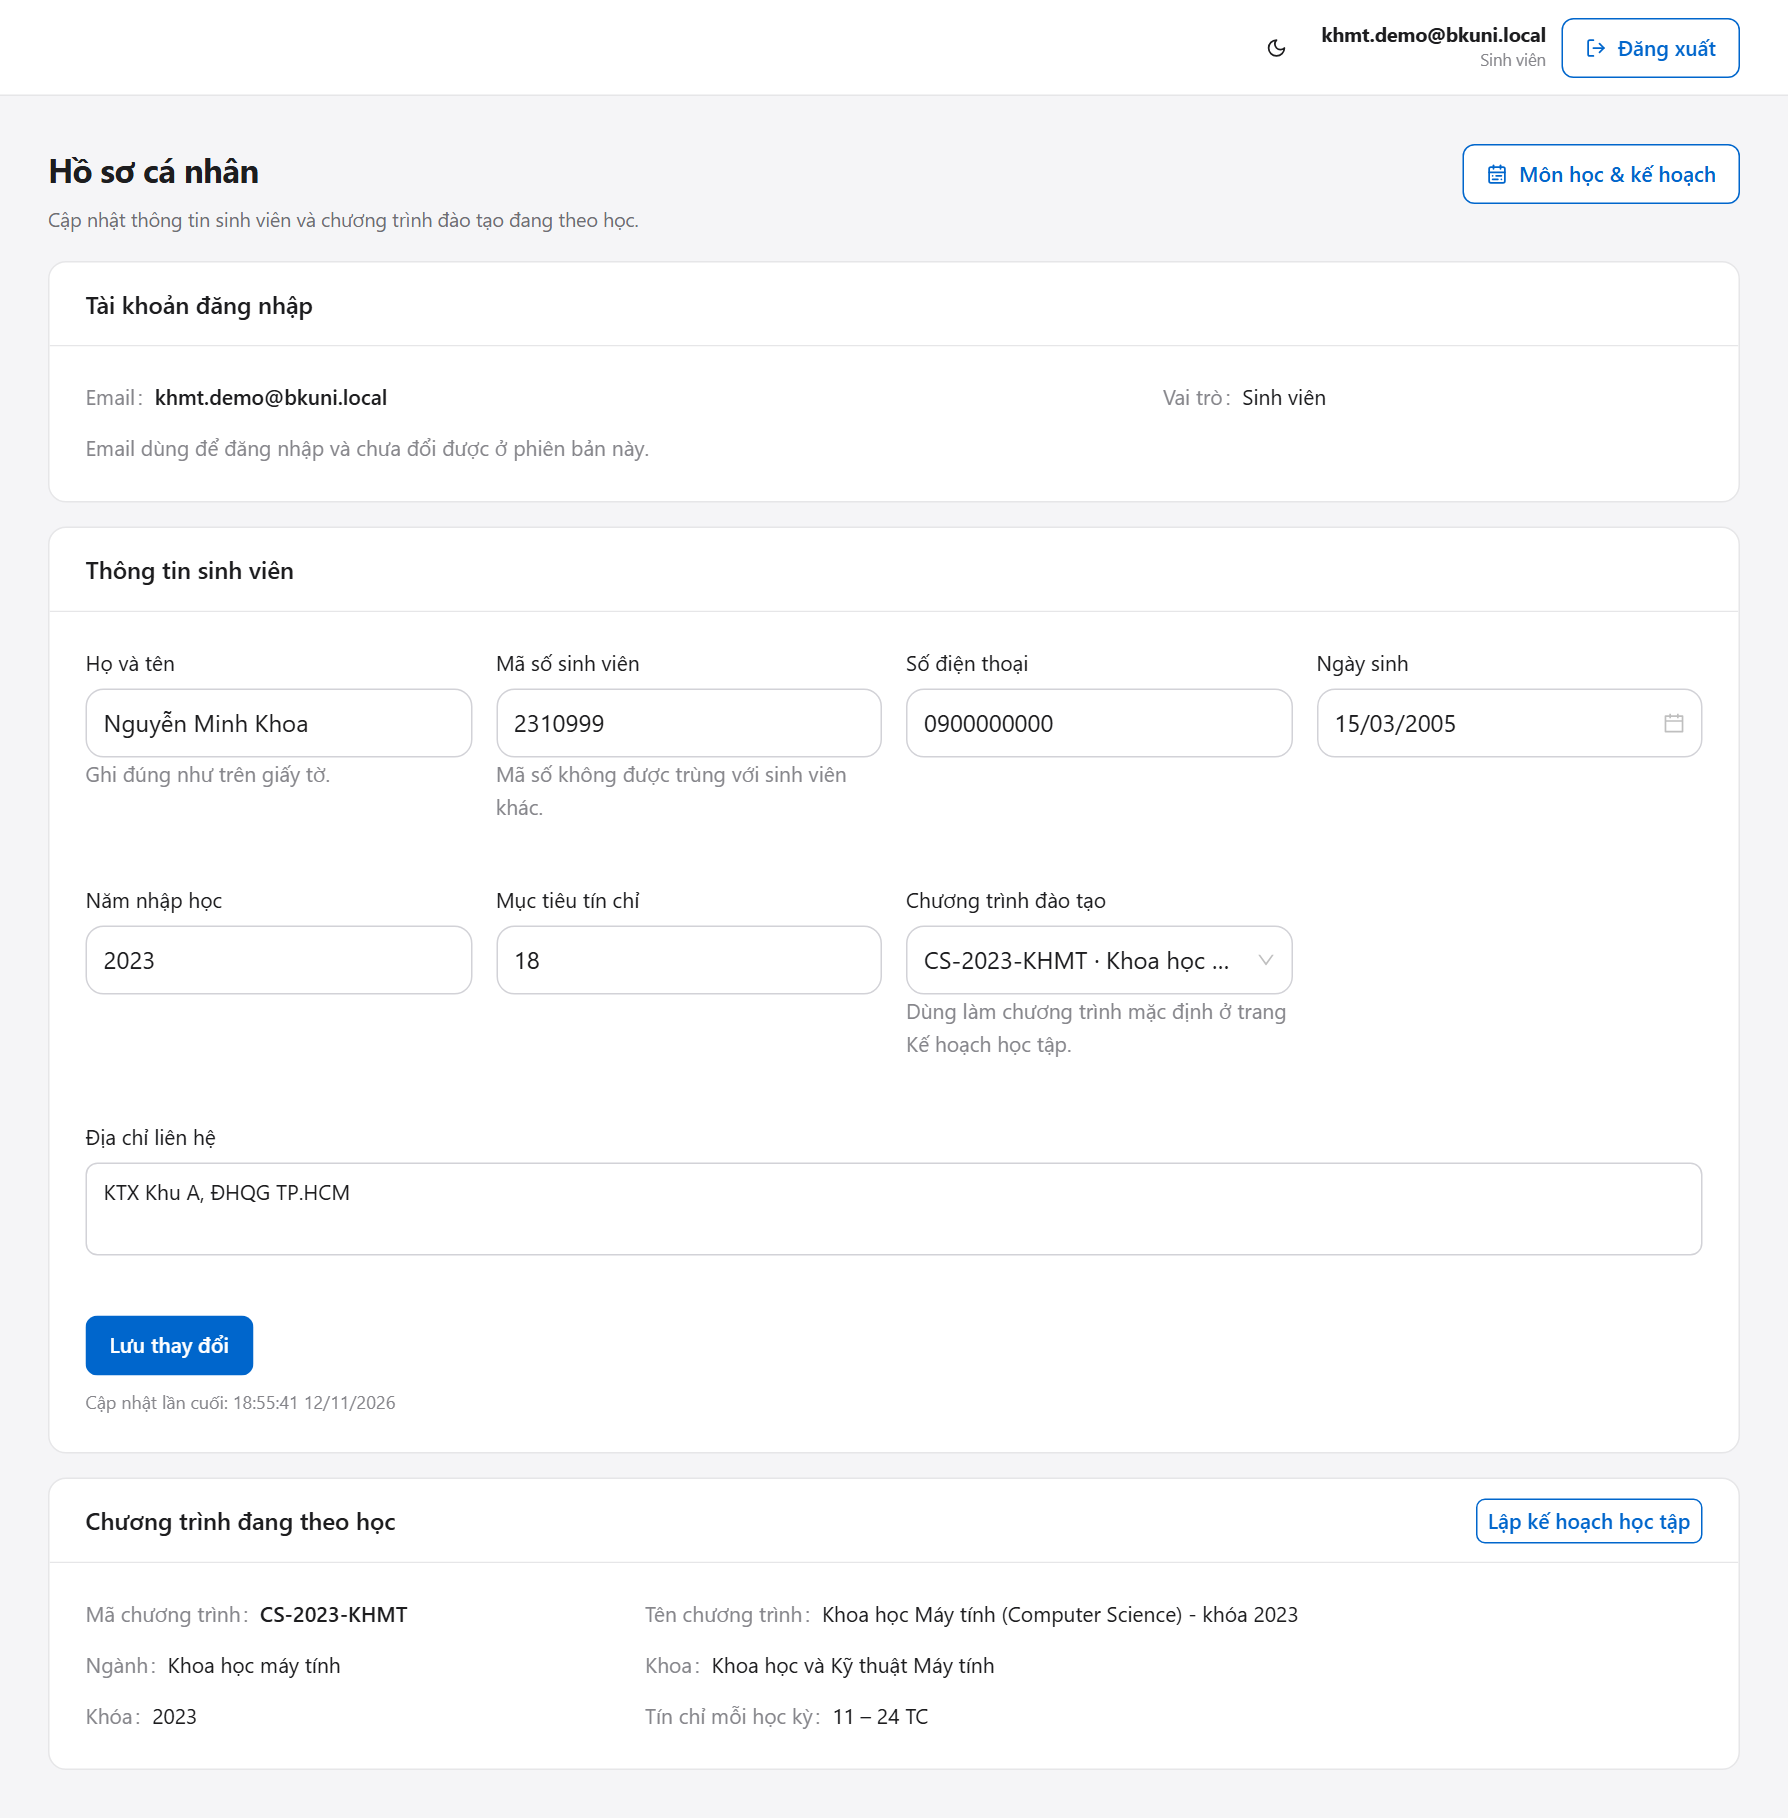
\includegraphics[width=\textwidth]{image/ui/profile.png}
    \caption{The Personal Profile page}
    \label{fig:ui-profile}
\end{figure}

\subsection{AI Advisor: Retrieval-Augmented Generation}
\label{subsec:rag}

This section specifies the algorithm behind the AI Advisor page presented in Section~\ref{subsec:ui-design}. The advisor answers open-ended questions in natural language, such as which elective fits a specialization, whether a course is heavy, or how to balance a semester. A large language model (LLM) plans a \emph{trajectory} of tool calls that retrieve the Student's analysis results and curriculum data, and then writes an answer that the backend validates before showing it. The advisor follows a strict division of labour with the rule-based code of the system (Section~\ref{subsubsec:architecture-overview}): the progress analysis computed from curriculum rules is the source of truth for eligibility, outstanding requirements and bottleneck courses, while the LLM explains, prioritizes and asks follow-up questions. The advisor never decides on its own whether a Student may take a course; it reads that decision from the analysis results.

\subsubsection{Motivation and Design Principles}

An LLM on its own is unsuitable for academic advising. It does not know a specific curriculum, it may invent course codes, credit values or prerequisite relations, and its answers cannot be checked. Retrieval-Augmented Generation (RAG) addresses this by retrieving relevant information from a trusted source and placing it in the model's context before the answer is generated.

Classic RAG retrieves text passages from a vector index by embedding similarity. BK Uni uses an \emph{agentic, tool-based} variant instead, because its knowledge is mostly structured and relational (courses, rules, groups, statuses, offering history) and must be exact rather than merely similar. The model is given a set of tools, each backed by a database query or by the analysis results, and decides during the conversation which tools to call and with which arguments. The design follows four principles:
\begin{itemize}
    \item \textbf{Grounding:} every course code, name, credit value or rule mentioned in an answer must come from the context or from a tool result (FR-7.2).
    \item \textbf{Separation of decision and explanation:} eligibility, outstanding requirements and bottleneck courses are computed by rule-based code and given to the model as facts; the model only interprets them.
    \item \textbf{Mixed initiative:} when information is missing or several reasonable options exist, the model asks the Student a structured question instead of choosing on the Student's behalf (FR-7.3).
    \item \textbf{Verifiability:} the final answer is structured data checked by the backend, and the whole trajectory that led to it is stored, so every answer can be audited afterwards.
\end{itemize}

\subsubsection{Retrieval Sources}

The information available to the model in a turn comes from three layers, ordered from the most general to the most specific:
\begin{enumerate}
    \item \textbf{System prompt (domain knowledge).} A fixed instruction that defines the advisor's role and encodes domain knowledge that cannot be inferred from the data: the meaning of prerequisite, prior and corequisite relations; how specializations are obtained (a Student keeps a specialization only while every elective taken from the base group belongs to its list); how physical-education requirements are satisfied by concrete sports courses; and the priority order for recommendations (failed courses to retake, overdue required courses, bottleneck courses that unlock many others, required courses on schedule, then electives), capped by the semester's credit limit.
    \item \textbf{Analysis context (the Student's state).} A compact JSON summary of the Student's learning analysis, attached to the user message inside a \texttt{<context>} block. It contains the current and next semester, credit overview and capacity, warnings, failed and overdue courses, the number of required courses left, elective-group and specialization progress, the list of courses eligible for the next semester, the top bottleneck courses, the next step of the roadmap and unmet graduation regulations. To save tokens, the context is re-sent only when the analysis changes: the backend stores a SHA-256 hash of the full analysis with the conversation and attaches a new context block only when the hash differs.
    \item \textbf{Tools (details on demand).} Everything that does not fit in the summary is retrieved through the tools in Table~\ref{tab:advisor-tools}, which the model may call several times and in parallel within a turn.
\end{enumerate}

\begin{longtable}{|>{\raggedright\arraybackslash}p{0.32\textwidth}|>{\raggedright\arraybackslash}p{0.19\textwidth}|>{\raggedright\arraybackslash}p{0.39\textwidth}|}
\caption{Tools available to the AI advisor}
\label{tab:advisor-tools}\\
\hline
\textbf{Tool} & \textbf{Data source} & \textbf{Purpose} \\
\hline
\endfirsthead
\hline
\textbf{Tool} & \textbf{Data source} & \textbf{Purpose} \\
\hline
\endhead
\texttt{get\_analysis\_section} & Analysis results & Returns one section of the analysis in full (for example \texttt{eligible\_next}, \texttt{blocked\_next} with missing courses, \texttt{electives}, \texttt{roadmap}); the primary source for eligibility and progress. \\
\hline
\texttt{get\_course\_detail} & Database & Course information, recommended semester, prerequisite, prior and corequisite relations with the Student's status for each related course, courses it unlocks, containing elective groups and specializations, and offering history. \\
\hline
\texttt{check\_offering} & Offering history (myBK) & Whether up to 30 courses are offered in a given semester; confirmed when the semester's data exists, predicted otherwise. \\
\hline
\texttt{get\_course\_outline} & Course outlines (myBK) & Condensed course outline: objectives, weekly content, learning outcomes, grading scheme, exam format, study hours, materials, and outline conditions placed next to curriculum conditions. \\
\hline
\texttt{search\_curriculum\_\allowbreak courses} & Database and outlines & Searches the Student's curriculum by code, name keyword or topic in the outline content (accent-insensitive), returning statuses, groups and specializations. \\
\hline
\texttt{get\_specialization\_\allowbreak detail} & Database & Courses of a specialization, grouped by block with the required number of courses or credits, together with the Student's status for each course. \\
\hline
\texttt{search\_\allowbreak outlines} & Search index (or database) & Full-text search over the whole content of the course outlines, by topic, skill or tool, ranked by relevance with highlighted excerpts; can be limited to the Student's curriculum and filtered by laboratory work, projects or final-exam format. \\
\hline
\texttt{find\_similar\_\allowbreak courses} & Search index & Courses whose outlines are closest in content to a given course, with the characteristic keywords of that course; used for alternatives within an elective group or for what to study next. \\
\hline
\texttt{get\_senior\_free\_\allowbreak elective\_tips} & Curated list and database & Free-elective courses recommended by students of earlier cohorts (unofficial experience), with their credits, next-semester offering, the Student's status, and the free-elective requirement of the curriculum. \\
\hline
\texttt{submit\_answer} & -- & Submits the final structured answer; must be called exactly once to end the turn. \\
\hline
\end{longtable}

All tools are read-only and run inside the backend under the identity of the current Student. Their arguments only select what to read, never whose data, because the Student and the curriculum are fixed by the authenticated session rather than chosen by the model. Each tool result is serialized as JSON and truncated to 16{,}000 characters before being returned to the model.

When the offering data of the target semester is not yet available, \texttt{check\_offering} predicts it from the four most recent semesters of the same type (first semester, second semester or summer) for which data exists. Let $h$ be the number of those semesters in which the course was opened. The verdict is \emph{likely} if $h \ge 3$, \emph{uncertain} if $1 \le h \le 2$, \emph{unlikely} if $h = 0$ but the course has been opened in a semester of that type before, and \emph{never} if it has not. The advisor is instructed to present these verdicts as predictions from history, not as an official timetable.

\subsubsection{Agent Trajectory}

A conversation is a sequence of \emph{turns}, and each turn produces a \emph{trajectory}: an ordered list of steps
\[
  \tau = \langle s_1, s_2, \dots, s_n \rangle,
\]
where each step $s_i$ has one of the roles \texttt{system}, \texttt{context}, \texttt{user}, \texttt{assistant}, \texttt{tool}, \texttt{answer} or \texttt{error}. An \texttt{assistant} step holds the model's output for one call: its visible content, its reasoning trace and the tool calls it requested, together with token usage and latency. A \texttt{tool} step holds the name, arguments, result and execution time of one tool call. The turn ends with exactly one \texttt{answer} step, or with an \texttt{error} step if it could not be completed. Algorithm~\ref{alg:advisor-turn} describes how a turn is executed.

\begin{algorithm}[H]
\caption{One turn of the AI advisor}
\label{alg:advisor-turn}
\KwIn{Student $u$, conversation $c$ with stored steps $\tau_{\mathit{prev}}$, question $q$, analysis $A$}
\KwOut{Validated answer $a$, appended to $c$ as new steps}
$M \leftarrow \textsc{Replay}(\tau_{\mathit{prev}})$\tcp*{rebuild message history}
\If{$c$ has no system step}{record and prepend the system prompt to $M$}
\If{$\mathrm{SHA256}(A) \neq c.\mathit{hash}$}{
  $x \leftarrow \textsc{Summarize}(A)$; record a \texttt{context} step; $c.\mathit{hash} \leftarrow \mathrm{SHA256}(A)$\;
}
append $q$ (wrapped with $x$ if present) to $M$ and record a \texttt{user} step\;
$\mathit{rejected} \leftarrow \mathit{false}$\;
\For{$r \leftarrow 1$ \KwTo $R_{\max}=8$}{
  $\mathit{res} \leftarrow \textsc{LLM}(M, \mathit{tools})$; record an \texttt{assistant} step; append $\mathit{res}$ to $M$\;
  \If{$\mathit{res}$ requests no tool call}{
    $d \leftarrow \mathit{res}.\mathit{content}$\tcp*{plain-text draft}
    \textbf{break}\;
  }
  \ForEach{tool call $(f, \mathit{args}) \in \mathit{res}$}{
    \eIf{$f = \texttt{submit\_answer}$}{
      $(a, E) \leftarrow \textsc{Validate}(\mathit{args}, \mathit{lenient}=\mathit{rejected})$\;
      \lIf{$a$ is accepted}{$\mathit{out} \leftarrow \{\mathit{ok}\}$}
      \lElse{$\mathit{out} \leftarrow E$; $\mathit{rejected} \leftarrow \mathit{true}$}
    }{
      $\mathit{out} \leftarrow \textsc{Execute}(f, \mathit{args}, u)$\;
    }
    record a \texttt{tool} step; append $\textsc{Truncate}(\mathit{out})$ to $M$\;
  }
  \lIf{an answer $a$ was accepted}{record an \texttt{answer} step and \Return{$a$}}
}
$a \leftarrow \textsc{FormatJson}(d, q, \text{tool results of this turn})$\tcp*{fallback}
record an \texttt{answer} step and \Return{$a$}\;
\end{algorithm}

Within one round the model may request several tool calls at once, for example \texttt{check\_offering} for all candidate courses together with \texttt{get\_course\_outline} for the ones whose workload matters. A typical trajectory therefore has two or three rounds: the model reads the context, retrieves the details it needs, and submits its answer. The bound $R_{\max} = 8$ prevents a model that keeps calling tools from running indefinitely. Any exception raised while the turn is being executed, including an unreachable or timed-out AI service, is recorded as an \texttt{error} step, and no answer is fabricated (FR-7.6).

\subsubsection{Answer Validation and Enrichment}

The final answer is not free text but a JSON object passed as the argument of \texttt{submit\_answer}, with four fields:
\begin{itemize}
    \item \texttt{message}: a short answer in Vietnamese, with light formatting;
    \item \texttt{recommendations}: a list of courses, each with a code, a one- or two-sentence reason and a priority (\emph{high}, \emph{medium} or \emph{low});
    \item \texttt{choices}: structured follow-up questions of type \emph{single}, \emph{multiple} or \emph{text}, each option with a short description of its consequences;
    \item \texttt{suggestions}: up to three useful follow-up questions.
\end{itemize}

The backend first normalizes this object against the schema and then \emph{enriches} each recommendation with facts computed by code rather than by the model: the course name and credits from the database, whether the course belongs to the curriculum, its eligibility and missing conditions from the analysis results, its offering verdict for the next semester, and a short summary of its course outline. The interface displays these verified facts next to the model's reason, so a wrong statement in the reason is easy to spot.

Validation includes a self-correction step. If the answer refers to a course code that does not exist or violates the schema, the first submission is rejected and the list of errors is returned to the model as the tool result, so it can correct itself in the next round. If a later submission still contains errors, it is accepted \emph{leniently}: the invalid parts are dropped and a note stating what was removed is attached, so that a single wrong code does not discard an otherwise useful answer.

If the model ends a round with plain text instead of calling \texttt{submit\_answer}, or reaches the round limit, a fallback formatter is used. The backend makes a separate call in JSON mode, with reasoning disabled, that receives the Student's question, the draft answer and the tool results collected during the turn as evidence, and asks for the same schema. The result goes through the same validation. If two attempts fail, the draft text is returned with a note saying it could not be structured. Each answer records whether it came from \texttt{submit\_answer} or from the fallback formatter.

\subsubsection{Trajectory Persistence and Replay}

Every step is stored as soon as it is produced in the \texttt{advisor\_steps} table, ordered by a per-conversation sequence number that is unique within the conversation. This serves three purposes. First, it is the conversation memory: at the start of each turn the message history is rebuilt from the stored steps rather than kept in server memory, so a conversation can be continued at any time, even after the server restarts (FR-7.5). Second, it makes answers auditable: for any answer, it is possible to see exactly which data the model saw, which tools it called with which arguments, what they returned, and how long each step took (NFR-7). Third, the recorded token counts, including tokens served from the provider's prompt cache, make the cost and latency of the advisor measurable.

Replay applies a few rules so that the rebuilt history is always valid for the provider's API:
\begin{itemize}
    \item the model's reasoning trace is kept with each assistant message, as the provider requires when reasoning and tool calling are used together;
    \item calls to the fallback formatter are not part of the main dialogue and are skipped;
    \item a tool call that never received a result, for example because the previous turn failed, is closed with a synthetic ``interrupted'' result;
    \item two consecutive user messages, which occur when a previous turn failed before the model replied, are merged into one;
    \item a context block is replayed together with the user message it was attached to.
\end{itemize}
Finally, only one turn may run on a conversation at a time; a second request on the same conversation is rejected until the first finishes, so the step sequence never interleaves. This lock is kept in the memory of the Backend process, which is sufficient for the current single-instance deployment; running several Backend instances would require moving it to the database or a shared cache.

\subsubsection{Mixed-Initiative Interaction}

When the model returns \texttt{choices}, the interface renders them as selectable options. The Student's selections are sent back with the next message and formatted as a ``choice answers'' block that lists each question with the chosen values or free text. The model then continues advising based on these choices. This lets the advisor fill in information it cannot infer on its own, such as a target specialization, the number of credits the Student is willing to take, or whether summer study is an option. It also keeps decisions with real consequences, such as giving up a specialization by taking an elective outside its list, in the Student's hands.


% Hai mục tiếp theo của chương 3 (3.5 CSP Formulation, 3.6 ASP Encoding), nối tiếp mục RAG
\subsection{CSP Formulation}\label{sec:formulation}
\subsubsection{Motivation: Why a CSP?}\label{sec:motivation}
Both validating and recommending an academic plan need a representation of the curriculum rules. Two representations are common in the literature. We explain why neither fits our setting, and why we formulate the problem as a constraint satisfaction problem (CSP) instead.

\paragraph{Course prerequisite graph (CPG)}
A CPG has one node per course and one edge per prerequisite relation. From it, a planner can derive a valid order of courses, find the longest chain of dependent courses and suggest the next courses along a path. The value of a CPG therefore depends on the \emph{density} of its edges: when most courses are linked to others, the graph carries a lot of information about which course should come when. In our target university, only a few courses have prerequisite or
corequisite relations (assumption A2). The graph is then sparse, made of a few short chains and many isolated courses, and it says little about when most courses should be taken. Moreover, most of the rules we must check (credit load, level, offerings, credit totals, categories, GPA) are not
relations between two courses, so they cannot be edges at all.

\paragraph{Graph of sub-requirements}
Parameswaran, Venetis and Garcia-Molina~\cite{parameswaran-2011} express degree requirements as a structured set of \emph{sub-requirements} over courses (for example, ``at least two courses from this list'') and recommend plans that satisfy them. This representation is expressive and handles complex rules well. Its cost is the modelling effort: curriculum experts must write the sub-requirements of each programme and verify that they match the regulations, and must redo this when the curriculum changes. We do not want the system to depend on such expert-made structures. It should be set up from information that already exists in the curriculum documents.

\paragraph{Constraint satisfaction}
A CSP takes the opposite route. We do not describe the structure of a good plan. We only state \emph{variables} (which course is taken when), \emph{domains} (whether the fact that a certain course is taken is true or not) and \emph{constraints} (the rules), and a solver searches for plans that satisfy them. The data needed are those already found in the regulations: the course list, credits, prerequisite lists and thresholds (Section~\ref{sec:inputs}). This gives us the following advantages.
\begin{itemize}
      \item \textbf{No density requirement.} A prerequisite is one constraint among others. The model works the same with few or many relations.
      \item \textbf{No expert-made structure.} The constraints are written once in a general form, and each curriculum only supplies data.
      \item \textbf{One model, several uses.} The same constraints support generating a plan, checking a student's draft and repairing it (Section~\ref{sec:scope}), which is what a mixed-initiative system needs~\cite{wu-thesis}.
      \item \textbf{Easy to extend.} A new rule, such as equivalent courses, is a new constraint and does not change the structure of the model.
      \item \textbf{Hard and soft requirements are separated.} Rules that must hold are constraints, while goals and preferences are objectives.
\end{itemize}

\paragraph{Disadvantages in our choice}
A CSP finds plans that \emph{satisfy the rules}. It does not by itself know which plan is educationally good, which a well-connected graph or an expert-made structure may hint at. We address this through the objectives (Section~\ref{sec:objectives}). Solving a general CSP is hard in the worst
case, but the instances here (tens to hundreds of courses and a handful of semesters) are small by solver standards.


\subsubsection{Overview and Scope}\label{sec:scope}
The task is to recommend, for every remaining semester, which courses a student should take so that all curriculum rules are respected and the student graduates. We formulate it as a CSP, following the mixed-initiative view of an academic plan~\cite{wu-thesis}: the student may pre-fill part of
a course--semester matrix, and the system completes, checks or repairs the rest. In Section~\ref{sec:encoding} the CSP is \emph{encoded} as an answer set program and solved with \texttt{clingo}.

The formulation supports three modes:
\begin{description}
      \item[Generate.] Given the history and the student's pins and bans, find the best feasible plan.
      \item[Check.] Given a complete draft plan, do not search. Report every violated constraint together with the course and semester involved.
      \item[Repair.] Given a draft plan that violates some constraints, find a feasible plan that differs from the draft in as few cells as possible. The difference between the two matrices tells the student \emph{how to resolve} the problem.
\end{description}

\paragraph{Planning scope}
The plan is computed for the \emph{whole remaining horizon at once}, not one semester after another. Graduation is a global condition: a semester-by-semester planner may choose a course early that later makes a prerequisite chain, an offering or the credit target unreachable, and a repair may need to change a semester far from the violation. The system is still used in a rolling way: after each real semester, the
actual grades are added to the history and the remaining horizon is planned again. The recommendation for the next semester is the first planned column of the matrix, and showing only that column gives the semester-level view.

\paragraph{What needs to be formulated}
\begin{itemize}
      \item \textbf{Curriculum constraints.} One core function of the system is validation, so the rules of the curriculum must be modelled robustly. They include course-level rules (prerequisites, corequisites, credits of a course) and programme-level rules (load limits, level, and the requirements for graduation such as total credits, compulsory courses and English level). We distinguish \emph{semester constraints}, which hold in every planned semester, and \emph{graduation conditions}, which hold for the plan as a whole.
      \item \textbf{Curriculum data.} The facts that describe the curriculum. They are supplied once per programme and are the same for every student.
      \item \textbf{Student data.} The facts and decisions of one student: the course history, which is represented as a course--semester matrix, and the student's own choices.
\end{itemize}
Section~\ref{sec:inputs} defines these data precisely.

\paragraph{Notable characteristics of the problem}
\begin{itemize}
      \item \textbf{Hard and soft requirements.} Prerequisites, corequisites, credit limits and compulsory courses are strict yes/no conditions (feasibility conditions). Depending on the curriculum, more hard constraints can be added. In contrast, student preferences, the target GPA and the wish to graduate early are optimization objectives used to rank the admissible plans. No recommended plan therefore violates an academic rule, and the remaining freedom is used for the student's benefit.
      \item \textbf{Horizon.} The model plans the whole remaining horizon, and the next-semester recommendation is a view of that plan (see the planning scope above).
      \item \textbf{Uncertainty in future GPA.} Grades cannot be known before a course is completed. Pass/fail is therefore treated deterministically for structural rules (an attempt is assumed passed, assumption A1), while grade-dependent targets, such as the cumulative GPA, use expected grades and are soft.
      \item \textbf{Retake policy.} Institutions usually count the grade of a retaken course in one of two ways: the \emph{highest} grade counts or the \emph{latest} grade counts. The policy is a parameter of the curriculum. A retake costs load and money in its semester, but its credits are earned only once.
      \item \textbf{External requirements.} Requirements that do not depend on courses (English level, volunteering days, etc.) are treated as given facts and checked only at graduation (Section~\ref{sec:graduation}).
\end{itemize}

% The constraints fall into three groups:
% \begin{itemize}
%   \item \textbf{semester constraints} (C1--C7), which must hold in every planned semester;
%   \item \textbf{graduation conditions} (G1--G4), which must hold for the plan as a whole;
%   \item \textbf{objectives}, which choose the best plan among the feasible
%         ones.
% \end{itemize}

\paragraph{Hard and soft requirements}
Table~\ref{tab:classes} classifies all requirements. Only the student's own decisions may be relaxed when a plan has to be repaired.

\begin{table}[ht]
\centering
\small
\begin{tabular}{@{}p{3.3cm}p{5.2cm}p{4.6cm}@{}}
\toprule
\textbf{Class} & \textbf{Content} & \textbf{Treatment} \\
\midrule
Curriculum rules & C1, C2, C3, C4, C5 (load), C7 & always hard \\
Student decisions & pinned/banned cells, budget (C6), $T_{\max}$, retake permissions & hard when solving; may be relaxed in repair \\
Graduation goals & G1, G2, G3, external requirements & hard \\
Soft goal & G4 (GPA) & penalized \\
\bottomrule
\end{tabular}
\caption{Classification of the requirements.}
\label{tab:classes}
\end{table}

%%%%%%%%%%%%%%%%%%%%%%%%%%%%%%%%%%%%%%%%%%%%%%%%%%%%%%%%%%%%%%%%%%%%%%%%%%
\subsubsection{Assumptions}

\begin{description}
      \item[A1. Optimistic pass.] Every planned attempt is assumed to be passed, with a grade given by the student or by an external grade-prediction component. When planning semester $s$, the courses planned in earlier planned semesters are therefore treated as ``temporarily passed''. The prediction model itself is outside the scope of the formulation.
      \item[A2. Acyclic, sparse relations.] The prerequisite graph and the corequisite graph are acyclic, and each course has only a few direct relations. Both are therefore checked directly on each course, without computing transitive closures.
      \item[A3. Unique course identity.] Equivalent courses are either absent or resolved in preprocessing.
      \item[A4. History is data.] The grades of completed semesters are read-only input.
      \item[A5. Fixed horizon.] The student gives a maximum number of semesters $T_{\max}$ within which graduation must be reached.
\end{description}

\subsubsection{Input Data and Data Treatment}\label{sec:inputs}

The formulation works with three kinds of data. They differ in where they come from and how often they change.
\begin{description}
  \item[Index sets (defined by the system).] The sets that give the problem its size and shape: the set of courses and the set of semesters. They are not typed in. The system builds them from the other two kinds of data (Table~\ref{tab:index}).
  \item[Curriculum data (supplied by the institution).] Describes the programme. It is entered once, is the same for all students of the programme, and is never changed by the solver (Table~\ref{tab:curriculum}).
  \item[Student data (supplied per student).] Describes one student: the history, the student's decisions and constraints. It changes between sessions, and the history grows after every real semester (Table~\ref{tab:student}).
\end{description}

\begin{table}[ht]
\centering
\small
\begin{tabular}{@{}>{\raggedright\arraybackslash}p{3.9cm}>{\raggedright\arraybackslash}p{4.2cm}>{\raggedright\arraybackslash}p{5.2cm}@{}}
\toprule
\textbf{Symbol} & \textbf{Meaning} & \textbf{Built from} \\
\midrule
$C$ & set of courses & all courses in the curriculum data \\
$S=\{1,\dots,T_{\max}\}$ & set of semesters & horizon $T_{\max}$ given by the student \\
$s_0$ & last completed semester & number of semesters in the history matrix $H$ \\
$S_H=\{1,\dots,s_0\}$ & history semesters & $s_0$ \\
$S_P=\{s_0+1,\dots,T_{\max}\}$ & planned semesters & $s_0$ and $T_{\max}$ \\
\bottomrule
\end{tabular}
\caption{Index sets (defined by the system).}
\label{tab:index}
\end{table}

\begin{table}[ht]
\centering
\small
\begin{tabular}{@{}p{3.1cm}>{\raggedright\arraybackslash}p{10.2cm}@{}}
\toprule
\textbf{Symbol} & \textbf{Meaning} \\
\midrule
\multicolumn{2}{@{}l}{\emph{Course data (one entry per course)}} \\
$\mathrm{cr}(c)$ & credits of course $c$ \\
$\mathrm{lv}(c)$ & level of course $c$ ($1$--$4$) \\
$\mathrm{off}(c,s)$ & course $c$ is offered in semester $s$ \\
$\mathrm{pre}(c)$, $\mathrm{co}(c)$ & prerequisites and corequisites of $c$, each a conjunction of
clauses, a clause being a disjunction of courses (CNF) \\
$C_{\mathrm{comp}}$ & compulsory courses \\
$G_j$ & category (group) $j$: the set of courses that belong to it \\
\midrule
\multicolumn{2}{@{}l}{\emph{Programme regulations}} \\
$g_{\mathrm{pass}}$ & lowest passing grade \\
$L_{\min}, L_{\max}$ & minimum and maximum load per semester (credits) \\
$\mathrm{Cr}_{\min}$, $\theta$ & credits and cumulative GPA required to graduate \\
$r_j$ & credits required from category $G_j$ \\
$\mathrm{fee}(L)$ & tuition fee of a semester with load $L$ credits \\
$\lambda(E)$ & student level given $E$ earned credits \\
$\rho$ & retake policy: \emph{highest} or \emph{latest} grade counts \\
$K_{\mathrm{ext}}$ & list of external graduation requirements (their status is student data) \\
\bottomrule
\end{tabular}
\caption{Curriculum data (supplied by the institution).}
\label{tab:curriculum}
\end{table}

\begin{table}[ht]
\centering
\small
\begin{tabular}{@{}p{3.1cm}>{\raggedright\arraybackslash}p{10.2cm}@{}}
\toprule
\textbf{Symbol} & \textbf{Meaning} \\
\midrule
$H$ & course history as a course--semester matrix; $h(c,s)$ is the grade of $c$ in completed semester $s$ (empty if not attempted) \\
$\hat g(c)$ & expected grade for a planned attempt of $c$, given by the student or by a grade-prediction component \\
$T_{\max}$ & last semester in which the student may still study (horizon) \\
$b_s$ & tuition budget of the student for semester $s$ \\
$\mathrm{Pin}$, $\mathrm{Ban}$ & planned cells that the student insists on, or forbids \\
$\mathrm{Imp}$ & completed courses that the student allows to retake to improve the grade \\
$\mathrm{Ext}_k$ & true/false status of each external requirement $k\in K_{\mathrm{ext}}$ \\
$D$ & draft plan: the cells the student proposes (check and repair modes only) \\
\bottomrule
\end{tabular}
\caption{Student data (supplied per student).}
\label{tab:student}
\end{table}

\paragraph{Curriculum data as tables of facts}
Every item in Table~\ref{tab:curriculum} is entered as a table of facts: one row per course for credits and level, one row per course and semester for the offerings, and one row per (course, clause, alternative) for prerequisites and corequisites in CNF. The functions $\mathrm{fee}$, $\lambda$ and $\rho$ are deliberately abstract. For example, $\mathrm{fee}$ may be linear in the load, a flat rate with bands, or a table; only the interface ``load of a semester $\to$ money'' is fixed. The curriculum data are assumed to be
correct and complete. They come from the official curriculum documents, and checking their quality is outside the scope of this work.

\paragraph{Student history as a course--semester matrix}
The history is stored as a matrix $H$ whose rows are courses and whose columns are the completed semesters. The entry $h(c,s)$ is the grade the student obtained when taking $c$ in semester $s$, and is empty if the student did not take it. Failed attempts are kept (their grade is below
$g_{\mathrm{pass}}$), because they count for the load of that semester and may be retaken. A course taken in several semesters simply has several non-empty entries in its row. The matrix is never edited by the solver. It is only extended with the real grades after each semester.

\paragraph{History and plan form one matrix}
The plan is the same matrix extended to the planned semesters. The left block (history) is fixed by $H$. The right block (plan) is what the solver completes, except that pinned cells are fixed to ``taken'' and banned cells to ``not taken''. Table~\ref{tab:matrix} shows an example. In check mode the draft $D$ is placed in the right block and only verified. In repair mode the draft is the reference from which the solution must differ as little as possible.

\begin{table}[ht]
\centering
\small
\begin{tabular}{@{}lcc@{\hspace{1.5em}}cc@{}}
\toprule
 & \multicolumn{2}{c}{History $S_H$ (fixed)} & \multicolumn{2}{c}{Plan $S_P$ (to complete)} \\
\cmidrule(lr){2-3}\cmidrule(lr){4-5}
\textbf{Course} & S1 & S2 & S3 & S4 \\
\midrule
MA101 & 3.0 & -- & ? & ? \\
CS101 & 0.0 & -- & ? & ? \\
CS102 & --  & -- & ? & ? \\
EL2   & --  & -- & 1 & 0 \\
\bottomrule
\end{tabular}
\caption{Example matrix with $s_0=2$ and $T_{\max}=4$. History entries are grades (``--'' means not attempted). In the plan block, ``?'' is a free cell decided by the solver, ``1'' a pinned cell and ``0'' a banned cell. Here the student passed MA101 and failed CS101 in semester 1.}
\label{tab:matrix}
\end{table}



\subsubsection{Variables and Domain}

The plan is the course--semester matrix described above: rows are courses and columns are semesters. Each cell is a variable
\[
  x_{c,s} \in \{0,1\}, \qquad c \in C,\ s \in S,
\]
where $x_{c,s}=1$ means that course $c$ is attempted in semester $s$.
Cells in the history ($s \in S_H$) are fixed by the student's record:
$x_{c,s}=1$ exactly when $h(c,s)$ is not empty.
Cells in the planned semesters ($s \in S_P$) are free, except that the
student may \emph{pin} a cell to $1$ (``I want this course here'') or
\emph{ban} it (``not this semester'').
Because several cells of the same row may equal $1$, retaking a course
needs no special modelling.

%%%%%%%%%%%%%%%%%%%%%%%%%%%%%%%%%%%%%%%%%%%%%%%%%%%%%%%%%%%%%%%%%%%%%%%%%%
\subsubsection{Derived Quantities}

The following quantities are functions of the matrix $x$.

\begin{itemize}
  \item \textbf{Pass.} $p_{c,s}=1$ if the course is passed in semester $s$:
        in the history when $h(c,s) \ge g_{\mathrm{pass}}$, and in a planned
        semester whenever $x_{c,s}=1$ (assumption A1).
  \item \textbf{Passed before / by.} $P^{<}_{c,s}=\bigvee_{s'<s} p_{c,s'}$ and
        $P^{\le}_{c,s}=\bigvee_{s'\le s} p_{c,s'}$.
  \item \textbf{Load.} $L_s=\sum_{c} \mathrm{cr}(c)\,x_{c,s}$.
        Every attempt counts, including retakes.
  \item \textbf{Earned credits.} A course earns its credits only on its
        first pass: $e_{c,s}=p_{c,s}\wedge\neg P^{<}_{c,s}$.
        The credits earned before semester $s$ are
        $E_s=\sum_{s'<s}\sum_c \mathrm{cr}(c)\,e_{c,s'}$.
  \item \textbf{Level.} The level of the student in semester $s$ is
        $\lambda(E_s)$. It uses credits earned \emph{before} $s$, which avoids
        a circular definition.
  \item \textbf{GPA.} For each attempted course, the counted grade
        $\gamma(c)$ follows the retake policy $\rho$ (using $h(c,s)$ for
        completed attempts and $\hat g(c)$ for planned ones). The cumulative GPA is
        $\sum_c \mathrm{cr}(c)\gamma(c)\big/\sum_c \mathrm{cr}(c)$, summed over attempted
        courses, each counted once.
\end{itemize}

The distinction between $L_s$ and $E_s$ implements the retake rule of the
curriculum: a retake costs load and money in its semester, but it adds
nothing to the credits needed for the level and for graduation.

%%%%%%%%%%%%%%%%%%%%%%%%%%%%%%%%%%%%%%%%%%%%%%%%%%%%%%%%%%%%%%%%%%%%%%%%%%
\subsubsection{Semester Constraints}

For every planned semester $s \in S_P$ and every course $c$ with $x_{c,s}=1$:

\begin{description}
  \item[C1. Offering.] $\mathrm{off}(c,s)$ must hold.
  \item[C2. Retaking.] Under the optimistic pass, repeating a course that
        is already passed in the plan is pointless, so a planned attempt of
        $c$ is allowed only if
        (a) $c$ was not attempted earlier in the plan, and
        (b) if $c$ was already passed in the history, the student has
        explicitly allowed a grade-improvement retake ($c\in\mathrm{Imp}$).
        A failed course in the history can be retaken freely.
  \item[C3. Prerequisites.] For every clause $K$ of $\mathrm{pre}(c)$, at least
        one course $a\in K$ has $P^{<}_{a,s}$, i.e.\ it was passed in
        \emph{any earlier} semester.
  \item[C4. Corequisites.] For every clause $K$ of $\mathrm{co}(c)$, at least
        one course $a\in K$ has $P^{\le}_{a,s}$, i.e.\ it was passed in an
        earlier \emph{or the same} semester.
  \item[C7. Level.] $\mathrm{lv}(c) \le \lambda(E_s)$.
\end{description}
For the semester as a whole:
\begin{description}
  \item[C5. Load.] $L_{\min}\le L_s\le L_{\max}$. The minimum is waived in
        the graduation semester $T$ (Section~\ref{sec:graduation}), and no
        course may be planned after $T$.
  \item[C6. Fee.] $\mathrm{fee}(L_s)\le b_s$.
\end{description}
(Constraint numbers follow the original list; the constraint on equivalent
courses was removed, see A3, and C1 was added.)

The CNF form allows both ``and'' and ``or'' relations. For example, a course
with $\mathrm{pre}=\text{CS101}\wedge(\text{MA101}\vee\text{MA102})$ needs
CS101 and at least one of the two mathematics courses.

%%%%%%%%%%%%%%%%%%%%%%%%%%%%%%%%%%%%%%%%%%%%%%%%%%%%%%%%%%%%%%%%%%%%%%%%%%
\subsubsection{Graduation Conditions}
\label{sec:graduation}

The \emph{graduation semester} $T$ is the first semester in which the
conditions G1--G3 and the external requirements all hold, counting everything
passed up to and including $T$. The plan must satisfy $T\le T_{\max}$.

\begin{description}
  \item[G1. Compulsory courses.] $P^{\le}_{c,T}$ holds for every $c\in C_{\mathrm{comp}}$.
  \item[G2. Total credits.] The credits earned up to $T$ are at least $\mathrm{Cr}_{\min}$.
  \item[G3. Categories.] For each group $G_j$, the credits earned from its
        courses up to $T$ are at least $r_j$.
  \item[G4. Cumulative GPA.] The cumulative GPA is at least $\theta$.
        This is a \emph{soft} condition because planned grades are only
        expected grades (see below).
\end{description}

\paragraph{External requirements}
Requirements that do not depend on the courses (English level, volunteering
days, \dots) are \emph{not} variables or constraints of the CSP. They enter
as true/false input facts $\mathrm{Ext}_k$, and graduation requires all of
them to be true. This keeps the CSP clean while keeping the whole program
runnable end to end.

\paragraph{GPA as a soft condition}
Planned courses have no real grades yet. The formulation therefore uses the
expected grades $\hat g(c)$ and measures the GPA \emph{shortfall}, i.e.\ by how
much the projected GPA is below $\theta$. The shortfall is penalized in the
objective and reported to the student as a warning. A prediction model that
supplies $\hat g(c)$ is a separate component and can be replaced without
changing the formulation.

%%%%%%%%%%%%%%%%%%%%%%%%%%%%%%%%%%%%%%%%%%%%%%%%%%%%%%%%%%%%%%%%%%%%%%%%%%
\subsubsection{Objectives}\label{sec:objectives}

Among all feasible plans, the system returns the best one under a
lexicographic order of objectives (Table~\ref{tab:objectives}). The student
may reorder or reweight them, which is itself a form of interaction.

\begin{table}[ht]
\centering
\small
\begin{tabular}{@{}cp{11.5cm}@{}}
\toprule
\textbf{Rank} & \textbf{Objective (minimize)} \\
\midrule
1 & number of cells changed with respect to the student's draft (repair mode only) \\
2 & graduation semester $T$ \\
3 & GPA shortfall \\
4 & number of planned retakes \\
5 & largest semester load (load balance) \\
\bottomrule
\end{tabular}
\caption{Default objective order.}
\label{tab:objectives}
\end{table}
\lstdefinelanguage{clingo}{
  morecomment=[l]{\%},
  morekeywords={not},
  sensitive=true
}
\lstdefinestyle{clingostyle}{
  language=clingo,
  basicstyle=\ttfamily\footnotesize,
  commentstyle=\color{gray}\itshape,
  keywordstyle=\color{blue!60!black},
  columns=fullflexible,
  keepspaces=true,
  breaklines=true,
  frame=single,
  framerule=0.3pt,
  rulecolor=\color{black!30},
  xleftmargin=2pt,
  xrightmargin=2pt,
  aboveskip=0.8em,
  belowskip=0.6em
}
\lstset{style=clingostyle}

%%%%%%%%%%%%%%%%%%%%%%%%%%%%%%%%%%%%%%%%%%%%%%%%%%5
% TAKE THIS SECTION AS AN EXAMPLE TO ASP ENCODING, THE REAL ASP PROGRAM IS STILL BEING TESTED.
%%%%%%%%%%%%%%%%%%%%%%%%%%%%%%%%%%%%%%%%%%%%%%%%%%
\subsection{ASP Encoding}
\label{sec:encoding}
% =====================================================================
 
\subsubsection{Design}
 
The formulation is encoded in the answer set programming language of
\texttt{clingo}. We use ASP, rather than a generic CSP library, because
sums, counting, optimization with priorities and conditional (``exists a
clause member'') reasoning are built into the language.
The program has the usual \emph{generate and test} shape:
a choice rule generates the free cells $x_{c,s}$, and the constraints reject
plans.
 
Three design decisions are worth stating.
\begin{enumerate}
  \item \textbf{Constraints are violation atoms.}
        Instead of writing each constraint as an integrity constraint, we
        derive an atom \texttt{viol(kind,C,S)} when it is broken, and add a
        single integrity constraint forbidding all violations. If the
        external atom \texttt{check\_mode} is true, the integrity constraint
        is switched off and the program reports the violations. This gives
        the check mode without a second program.
  \item \textbf{One program, three modes.} Generate mode needs no draft.
        Repair mode adds the draft as facts \texttt{prop(C,S)}, and the
        distance to it is the highest-priority objective. Check mode adds
        \texttt{check\_mode} and forces distance $0$.
  \item \textbf{Integers only.} \texttt{clingo} has no floating-point
        numbers, so grades are stored in points $\times 100$
        ($3.00\to300$) and the GPA test is written by cross-multiplication:
        $\sum \mathrm{cr}\cdot\gamma \ge \theta \sum \mathrm{cr}$.
\end{enumerate}
 
The encoding is split into three files: \texttt{core.lp} (the formulation),
\texttt{data.lp} (the curriculum) and \texttt{student.lp} (history, expected
grades, budget). Table~\ref{tab:mapping} shows where each part of the
formulation lives.
 
\begin{table}[ht]
\centering
\small
\begin{tabular}{@{}p{4.2cm}>{\raggedright\arraybackslash}p{8.8cm}@{}}
\toprule
\textbf{Formulation} & \textbf{Encoding} \\
\midrule
Variable $x_{c,s}$ & choice rule \texttt{take(C,S)} for $s>s_0$; history in \texttt{hist(C,S,G)} \\
Pass, $P^{<}$, $P^{\le}$ & \texttt{pass}, \texttt{passed\_before}, \texttt{passed\_upto} \\
Load $L_s$, earned $E_s$, level & \texttt{load}, \texttt{earned}, \texttt{earned\_before}, \texttt{lam} \\
C1--C7 & atoms \texttt{viol(offering,\dots)}, \texttt{viol(retake,\dots)}, \texttt{viol(prereq,\dots)}, \texttt{viol(coreq,\dots)}, \texttt{viol(maxload,\dots)}, \texttt{viol(minload,\dots)}, \texttt{viol(fee,\dots)}, \texttt{viol(level,\dots)} \\
G1--G3, $T$ & \texttt{gradok}, \texttt{first\_grad}; \texttt{viol(no\_grad,\dots)} \\
G4 (GPA) & \texttt{best}, \texttt{gpa\_pts}, \texttt{gpa\_cr}, \texttt{short} \\
Objectives & \texttt{\#minimize} statements with priorities \\
\bottomrule
\end{tabular}
\caption{Mapping from the formulation to the encoding.}
\label{tab:mapping}
\end{table}
 
\subsubsection{Core Program}
 
\paragraph{Parameters and variables}
Parameters are constants that can be overridden from the command line.
The fee function is a table from load to money.
\begin{lstlisting}
% ===== Parameters (overridable with -c name=value) =====
#const now       = 1.     % last completed semester
#const tmax      = 5.     % planning horizon
#const lmin      = 6.     % minimum load (credits)
#const lmax      = 9.     % maximum load (credits)
#const lcap      = 30.    % size of the fee table
#const passmark  = 100.   % passing grade, in points x 100
#const credreq   = 24.    % credits required to graduate
#const gpamin    = 250.   % required cumulative GPA (2.50 x 100)
#const feeunit   = 1000.  % fee per credit (example fee function)
#external check_mode.     % true => only report violations
#defined ext_req/1. #defined ext_ok/1. #defined improve/1.
#defined fixed/2. #defined banned/2. #defined prop/2.
 
sem(1..tmax).
fee(L, feeunit*L) :- L = 0..lcap.      % fee function: load -> money
\end{lstlisting}
\begin{lstlisting}
% ===== Variable: planned cells take(C,S) in {0,1} =====
{ take(C,S) : course(C), sem(S), S > now }.
\end{lstlisting}
 
\paragraph{Attempts, passes and credits}
A planned attempt passes by assumption A1 (\texttt{pass(C,S) :- take(C,S)}),
and only the first pass of a course is earned.
\begin{lstlisting}
% ===== Attempts, grades, passes =====
att(C,S)      :- hist(C,S,_).
att(C,S)      :- take(C,S).
grade(C,S,G)  :- hist(C,S,G).
grade(C,S,G)  :- take(C,S), exp(C,G).
pass(C,S)     :- hist(C,S,G), G >= passmark.
pass(C,S)     :- take(C,S).                       % optimistic pass
 
passed_before(C,S) :- pass(C,S0), sem(S), S0 < S.
passed_upto(C,S)   :- pass(C,S0), sem(S), S0 <= S.
hist_passed(C)     :- hist(C,S,G), G >= passmark.
plan_passed_before(C,S) :- take(C,S0), S0 > now, sem(S), S0 < S.
attempt_before(C,S)     :- att(C,S0), sem(S), S0 < S.
\end{lstlisting}
\begin{lstlisting}
% ===== Load, earned credits, level =====
load(S,L)  :- sem(S), L = #sum{ Cr,C : att(C,S), credits(C,Cr) }.
earned(C,S) :- pass(C,S), not passed_before(C,S).  % first pass only
earned_before(S,E) :- sem(S),
    E = #sum{ Cr,C : earned(C,S0), S0 < S, credits(C,Cr) }.
earned_upto(S,E)   :- sem(S),
    E = #sum{ Cr,C : earned(C,S0), S0 <= S, credits(C,Cr) }.
lam(S,L) :- earned_before(S,E), lvl_range(L,Lo,Hi), Lo <= E, E < Hi.
\end{lstlisting}
 
\paragraph{Graduation and GPA}
\texttt{first\_grad(T)} is the graduation semester. The retake policy
``highest grade counts'' is written with \texttt{better} and \texttt{best};
the policy ``latest grade counts'' only changes these two rules.
\begin{lstlisting}
% ===== Graduation =====
miss_comp(S) :- sem(S), comp(C), not passed_upto(C,S).
miss_grp(S)  :- sem(S), reqgrp(G,R),
    #sum{ Cr,C : earned(C,S0), S0 <= S, ingroup(C,G), credits(C,Cr) } < R.
ext_fail     :- ext_req(X), not ext_ok(X).
gradok(S)    :- earned_upto(S,E), E >= credreq,
                not miss_comp(S), not miss_grp(S), not ext_fail.
first_grad(T) :- gradok(T), not gradok(S) : sem(S), S < T.
\end{lstlisting}
\begin{lstlisting}
% ===== GPA (retake policy: highest grade counts) =====
better(C,G) :- grade(C,_,G), grade(C,_,G2), G2 > G.
best(C,G)  :- grade(C,_,G), not better(C,G).
gpa_pts(P) :- P = #sum{ G*Cr,C : best(C,G), credits(C,Cr) }.
gpa_cr(Q)  :- Q = #sum{ Cr,C : best(C,_), credits(C,Cr) }.
short(D)   :- gpa_pts(P), gpa_cr(Q), D = gpamin*Q - P, D > 0.
\end{lstlisting}
 
\paragraph{Constraints}
Prerequisites and corequisites are given in CNF as facts
\texttt{pre(C,K,A)}: course \texttt{C} has clause \texttt{K} containing
alternative \texttt{A}. A clause is satisfied when some alternative is
passed in time (\texttt{presat}, \texttt{cosat}).
\begin{lstlisting}
% ===== Constraints, written as violation atoms =====
presat(C,K,S) :- pre(C,K,A), passed_before(A,S).
cosat(C,K,S)  :- co(C,K,A),  passed_upto(A,S).
 
viol(offering,  C,S) :- take(C,S), not offered(C,S).
viol(retake,    C,S) :- take(C,S), plan_passed_before(C,S).
viol(retake,    C,S) :- take(C,S), hist_passed(C), not improve(C).
viol(prereq,    C,S) :- take(C,S), pre(C,K,_), not presat(C,K,S).
viol(coreq,     C,S) :- take(C,S), co(C,K,_),  not cosat(C,K,S).
viol(level,     C,S) :- take(C,S), level(C,V), lam(S,L), V > L.
viol(maxload,   0,S) :- load(S,L), S > now, L > lmax.
viol(minload,   0,S) :- load(S,L), S > now, first_grad(T), S < T, L < lmin.
viol(fee,       0,S) :- load(S,L), S > now, fee(L,F), budget(S,B), F > B.
viol(after_grad,C,S) :- take(C,S), first_grad(T), S > T.
viol(no_grad,   0,0) :- #count{ T : first_grad(T) } = 0.
 
:- viol(_,_,_), not check_mode.
\end{lstlisting}
\begin{lstlisting}
% ===== Student decisions =====
:- fixed(C,S), not take(C,S).
:- banned(C,S), take(C,S).
\end{lstlisting}
 
\paragraph{Repair distance and objectives}
In \texttt{clingo}, a larger priority number is more important, so the
distance to the draft has the highest priority (6) and the load balance the
lowest (2).
\begin{lstlisting}
% ===== Distance to a proposed plan (repair mode) =====
has_prop :- prop(_,_).
changed(C,S) :- prop(C,S), not take(C,S).
changed(C,S) :- take(C,S), not prop(C,S), has_prop.
:- changed(_,_), check_mode.
\end{lstlisting}
\begin{lstlisting}
% ===== Objectives (higher priority number = more important) =====
maxload(M) :- M = #max{ L : load(S,L), S > now }.
#minimize{ 1@6,C,S : changed(C,S) }.
#minimize{ T@5     : first_grad(T) }.
#minimize{ D@4     : short(D) }.
#minimize{ 1@3,C,S : take(C,S), attempt_before(C,S) }.
#minimize{ M@2     : maxload(M) }.
\end{lstlisting}
 
\subsubsection{Interaction}
 
The three modes are selected only by the input files:
\begin{lstlisting}[language={},basicstyle=\ttfamily\footnotesize]
clingo core.lp data.lp student.lp                         # generate
clingo core.lp data.lp student.lp draft.lp check.lp       # check
clingo core.lp data.lp student.lp draft.lp                # repair
\end{lstlisting}
where \texttt{draft.lp} lists the student's draft as \texttt{prop(C,S)} facts
and \texttt{check.lp} contains the single fact \texttt{check\_mode.}
Pins and bans are facts \texttt{fixed(C,S)} and \texttt{banned(C,S)}.
For a dialogue with the student, the same program can be driven from the
\texttt{clingo} Python API, which can toggle such facts as external atoms and
re-solve without grounding everything again.
 
% ===================================================================== The below section is NOT VERIFIED YET
% \subsection{Worked Example}
% \label{sec:example}
% % =====================================================================
 
% We run the encoding on a toy curriculum small enough to verify by hand.
% All results below were produced with \texttt{clingo} 5.8 and agree with the
% manual analysis.
 
% \subsubsection{Setting}
 
% \paragraph{Curriculum}
% Table~\ref{tab:toycourses} lists nine courses of $3$ credits each.
% The parameters are: $L_{\min}=6$, $L_{\max}=9$, $\mathrm{Cr}_{\min}=24$,
% $\theta=2.50$, $T_{\max}=5$, and $\mathrm{fee}(L)=1000\cdot L$.
% The level function is $\lambda(E)=1$ for $E<6$, $2$ for $6\le E<12$ and $3$
% for $E\ge 12$. At least $6$ credits must come from the elective group
% \{EL1, EL2, EL3\}. External requirements are assumed satisfied.
 
% \begin{table}[ht]
% \centering
% \small
% \begin{tabular}{@{}lccp{3.2cm}>{\raggedright\arraybackslash}p{4.4cm}@{}}
% \toprule
% \textbf{Course} & \textbf{Level} & \textbf{Compulsory} & \textbf{Offered} & \textbf{Relations} \\
% \midrule
% MA101 & 1 & yes & every semester & --- \\
% MA102 & 1 & no  & odd semesters  & pre: MA101 \\
% CS101 & 1 & yes & every semester & --- \\
% CS102 & 2 & yes & every semester & pre: CS101 $\wedge$ (MA101 $\vee$ MA102) \\
% CS201 & 2 & yes & every semester & pre: CS101; co: CS102 \\
% CS301 & 3 & yes & even semesters & pre: CS201 \\
% EL1, EL2 & 1 & no & every semester & --- \\
% EL3 & 2 & no & every semester & --- \\
% \bottomrule
% \end{tabular}
% \caption{Toy curriculum (all courses have 3 credits).}
% \label{tab:toycourses}
% \end{table}
 
% \paragraph{Student}
% The student has finished semester $1$ ($s_0=1$): MA101 passed with a B
% ($3.00$) and CS101 \emph{failed}, so CS101 must be retaken. The load of
% semester $1$ is $6$ credits but only $3$ credits are earned. Every planned
% course is expected to get a B.
 
% \subsubsection{Scenario 1: generating a plan}
 
% With a budget of $9000$ per semester (so the fee allows the full $9$
% credits), the solver returns the plan in Table~\ref{tab:plan1}, found as
% optimal with $T=4$. Several plans share the same optimal values; the
% solver returns one of them.
 
% \begin{table}[ht]
% \centering
% \small
% \begin{tabular}{@{}lccccc@{}}
% \toprule
% \textbf{Course} & \textbf{S1 (history)} & \textbf{S2} & \textbf{S3} & \textbf{S4} & \textbf{S5} \\
% \midrule
% MA101 & passed &        &        &        &  \\
% CS101 & failed & $\bullet$ &        &        &  \\
% EL1   &        & $\bullet$ &        &        &  \\
% MA102 &        &        & $\bullet$ &        &  \\
% CS102 &        &        & $\bullet$ &        &  \\
% CS201 &        &        & $\bullet$ &        &  \\
% CS301 &        &        &        & $\bullet$ &  \\
% EL2   &        &        &        & $\bullet$ &  \\
% \midrule
% \textbf{Load} & 6 & 6 & 9 & 6 & 0 \\
% \bottomrule
% \end{tabular}
% \caption{Optimal plan with budget $9000$ ($\bullet$ = planned attempt).}
% \label{tab:plan1}
% \end{table}
 
% The plan follows the constraints as expected. CS101 is retaken first
% because CS102 and CS201 depend on it. CS102 and CS201 share semester $3$,
% which is allowed because CS102 is a corequisite of CS201. CS301 is placed in
% semester $4$, the first even semester in which its prerequisite is passed.
% The earned credits are $3+21=24=\mathrm{Cr}_{\min}$, the elective group
% gets $6$ credits, one planned retake is used and the projected GPA is
% $3.00\ge 2.50$. The minimum load is waived in the graduation semester,
% and semester $5$ is empty.
 
% \subsubsection{Scenario 2: a tighter budget}
 
% If the budget drops to $6000$ per semester, the fee function limits the load
% to $6$ credits ($\mathrm{fee}(9)=9000>6000$). The chain CS101 $\to$ CS102/CS201
% $\to$ CS301 is unchanged, but the remaining $21$ credits no longer fit in
% three semesters, so the optimal plan graduates in semester $5$:
% S2 = \{CS101, EL1\}, S3 = \{CS102, CS201\}, S4 = \{CS301, EL2\} and
% S5 = \{MA102\}. MA102 is placed in semester $5$ because it is offered only
% in odd semesters, and its load of $3$ is below $L_{\min}$, which is allowed
% in the graduation semester.
 
% \subsubsection{Scenario 3: checking and repairing a draft}
 
% Suppose the student proposes, with the budget of $9000$:
% \[
%   \text{S2} = \{\text{CS101},\ \text{CS102},\ \text{EL1}\}, \qquad
%   \text{S3} = \{\text{CS201},\ \text{CS301},\ \text{EL2}\}.
% \]
 
% \paragraph{Check}
% The program reports the violations in Table~\ref{tab:viol}.
 
% \begin{table}[ht]
% \centering
% \small
% \begin{tabular}{@{}lp{9.5cm}@{}}
% \toprule
% \textbf{Violation} & \textbf{Reason} \\
% \midrule
% \texttt{prereq(cs102,2)} & CS101 is not yet passed before semester 2 (it was failed and is retaken in the same semester) \\
% \texttt{level(cs102,2)} & CS102 has level 2, but the student has earned only $3$ credits before semester 2 (level 1) \\
% \texttt{offering(cs301,3)} & CS301 is not offered in odd semesters \\
% \texttt{prereq(cs301,3)} & CS201 is planned in the same semester, not an earlier one \\
% \texttt{no\_grad} & the draft earns only $3+18=21<24$ credits and does not graduate within the horizon \\
% \bottomrule
% \end{tabular}
% \caption{Violations reported by the check mode.}
% \label{tab:viol}
% \end{table}
 
% \paragraph{Repair}
% The repair mode returns the feasible plan with the fewest changed cells:
% S2 = \{CS101, EL1\}, S3 = \{CS102, CS201, EL2\}, S4 = \{CS301, EL3\}, with
% $T=4$. Compared with the draft it changes $5$ cells:
% \begin{itemize}
%   \item move CS102 from semester 2 to semester 3 (2 cells);
%   \item move CS301 from semester 3 to semester 4 (2 cells);
%   \item add EL3 in semester 4 (1 cell), to reach the required credits.
% \end{itemize}
% These changes are the explanation given to the student. EL3 is chosen
% rather than MA102 because MA102 is offered only in odd semesters and
% semester $3$ is already full. If the budget of $6000$ of Scenario~2 applies to the
% same draft, the minimum repair needs $7$ changed cells and graduation moves
% to semester~$5$.
 
% \subsubsection{Summary}
 
% The example shows each part of the formulation at work: the retake counted
% in the load but not in the earned credits, CNF prerequisites, a corequisite
% in the same semester, the level and offering restrictions, the fee limiting
% the load, and the check and repair modes producing an explanation instead
% of a bare ``no plan''.


%\phantomsection % Tạo bookmark cho PDF
%\addcontentsline{toc}{section}{Tài liệu tham khảo} % Thêm vào Mục lục

%\bibliographystyle{ieeetr} 
%\renewcommand{\refname}{Tài liệu tham khảo}
%\bibliography{references} 
%\nocite{*}

% ===== KẾT THÚC =====


\end{document}
